
\documentclass[a4paper]{book}
\usepackage[utf8]{inputenc}

\usepackage{makeidx} 
\usepackage{graphicx}        
\graphicspath{{./}{Figure/}}
\usepackage{amsfonts,amsmath,amssymb}
\usepackage{multicol}       
\usepackage{subcaption}
\usepackage{cancel}
\usepackage{quoting}
\usepackage[bottom]{footmisc}
\usepackage[italian]{babel}
\usepackage{mathtools}
\usepackage{hyperref}
\hypersetup{
    colorlinks,
    citecolor=black,
    filecolor=black,
    linkcolor=black,
    urlcolor=black
}
\usepackage[utf8]{inputenc}
\usepackage{multirow}
\usepackage{siunitx}

\makeindex

\begin{document}

\author{Armenante Davide}

\title{Progetto di macchine\\ 
	\vspace{1cm}
	Appunti del corso}

\date{a.a. 2020 
	\vspace{2cm}
		\begin{figure}[h!]
			\centering
			\includegraphics[width=.8\textwidth]{fig/CarlinoPc.pdf}
			\label{}
		\end{figure}}
\maketitle

\frontmatter

%%%%%%%%%%%%%%%%%%%%%% pref_it.tex %%%%%%%%%%%%%%%%%%%%%%%%%%%%%%%%%%%%%
%
% Esempio di prefazione
%
% Usare questo file come template per il vostro documento.
%
%%%%%%%%%%%%%%%%%%%%%%%% Springer-Verlag %%%%%%%%%%%%%%%%%%%%%%%%%%

\preface

Prima che il lettore si immerga in questa appassionante lettura vorrei fare due precisazioni. L'impaginazione è tanto figa quanto il libro è scritto male, diffidate, non si tratta di un elaborato professionale ma di appunti presi a lezione. Apprezzate però, tutte le immagini sono state rifatte vettorialmente. Si ringraziano\footnote{Non avevo voglia di dedicare una pagina intera ai ringraziamenti per scrivere due righe, gli alberi ringraziano} soprattutto i revisori Carlo Pini\footnote{Detto CP7} e Fausto Dicech.



\tableofcontents

\mainmatter

% !TEX root = ../ProgettoMacchine2020.tex
% !TEX encoding = UTF-8 Unicode
% !TEX program = pdflatex
% !TEX spellcheck = it-IT
\chapter{Richiami teorici}
\section{Teoria della similitudine}
L’applicazione della teoria della similitudine costituisce un primo e potente strumento della progettazione, in particolar modo per quanto riguarda le turbomacchine. La teoria della similitudine permette di risolvere diversi problemi:
\begin{itemize}
\item[$-$] note le prestazioni di una macchina che ha determinate dimensioni,
si possono ricavare le prestazioni di una macchina geometricamente simile a quella considerata ma di diverse dimensioni nel dettaglio permette la realizzazione di prototipi in scala ridotta (esempio tipico: modellino della grande turbina idraulica che viene provato prima di procedere alla costruzione della macchina vera);
\item[$-$] nota una ben determinata condizione di funzionamento di una turbomacchina, come potrebbero essere le condizioni di progetto, si possono individuare altre condizioni di funzionamento ottenute variando la velocità di rotazione, la portata, oppure il lavoro scambiato (fluido/macchina);
\item[$-$] curve di prestazioni rilevate in determinate condizioni ambientali possono essere espresse in funzione di parametri che sono invarianti al variare delle condizioni ambientali stesse. Possiamo conoscere le prestazioni di una macchina operante in condizioni diverse (ad esempio un compressore sul livello del mare ad agosto e in montagna a Natale);
\end{itemize}
Accanto a tutti questi aspetti riguardanti la capacità di predire le prestazioni di una macchina, si ritrova anche un ausilio al designer in sede di progettazione. Con la teoria della similitudine si può stabilire in maniera semplice e veloce fin da subito quale sarà il tipo di macchina migliore da usare, quale sarà la sua geometria di base e quali le dimensioni generali. Grazie a ciò si riesce a sfruttare l’esperienza già maturata nella progettazione, sviluppo e test di altre macchine simili. Possedere un database ricco di informazioni relative a macchine pregresse risulta essere un vantaggio progettuale non di poco conto.


ll teorema di Buckingham (conosciuto anche come teorema pi greco), dovuto al fisico statunitense Edgar Buckingham, afferma:
\begin{quotation}
	Dato un problema descritto da un certo numero di equazioni in cui siano presenti $n$ variabili fisiche, se le dimensioni fondamentali di queste variabili sono $x$ allora il problema può essere completamente descritto da $n - x$ variabili adimensionali.
\end{quotation}
Per studiare il comportamento di una turbomacchina si definisce il seguente funzionale.
\begin{equation}
f(D_i,l_j,\dot{m},w,L_i,\mu,a_{01},\rho_{01})=0
\end{equation}
Con\\
$D_i$: serie di diametri rilevanti;\\
$l_j$: serie di lunghezze rilevanti;\\
$\dot{m}$: portata in massa;\\
$w$: velocità angolare;\\
$L_i$: lavoro ideale scambiato tra macchina e fluido per unità di massa;\\
$\mu$: viscosità dinamica del fluido;\\
$a_{01}$: velocità del suono all'ingresso in condizioni di ristagno;\\
$\rho_{01}$: densità del fluido.
\begin{equation}
Re= \frac{\rho_{01} w D^2}{\mu}
\end{equation}
\begin{equation}
Ma= \frac{w D}{a_{01}}
\end{equation}
Si evidenzia che tutti gli argomenti del funzionale sono descritti da una combinazione delle tre grandezze fondamentali M L T, ovvero massa lunghezza e tempo. Tenendo presente ciò è possibile adimensionalizzare gli argomenti del funzionale ottenendo una nuova espressione per lo stesso.

In una macchina termica in cui il fluido cambia le proprietà nei vari punti della macchina per definire la densità o la velocità del suono devo fissare
convenzionalmente una condizione rispetto alla quale vado a valutare quella
proprietà. 

Una condizione di riferimento che viene spesso adottata (non è
l’unica) potrebbe essere quella di valutare queste quantità nelle condizioni
totali all’ingresso della macchina (cioè condizioni valutate immaginando il fluido in quiete) che possiamo indicare con il pedice $01$ ($0$: condizioni totali o di ristagno; $1$: condizioni di ingresso).

<<<<<<< Updated upstream
Si può allo stesso modo definire le cifre di flusso $\varphi$ e di pressione $\psi$ andando ad adimensionalizzare rispettivamente la portata e il lavoro unitario:
=======
Si può allo stesso modo definire le cifre di flusso $\Phi$ e di pressione $\psi$ andando ad adimensionalizzare rispettivamente la portata e il lavoro unitario:
>>>>>>> Stashed changes
\begin{equation}
\varphi = \frac{\dot{m}}{\rho_{01}w D^3} \left( =\frac{Q}{w D^3} \right)
\end{equation}
\begin{equation}
\psi = \frac{L_i}{w^2 D^2}
\end{equation}
Il funzionale può essere espresso quindi secondo i numeri adimensionali:
\begin{equation}
f(\pi_i,\pi_j,\varphi,\psi,Re,Ma)=0
\end{equation}
Si può semplificare sotto le ipotesi di geometria simile.
\begin{equation}
f(\varphi,\psi,Re,Ma)=0
\end{equation}
Supponendo di confrontare due macchine se queste hanno le gli stessi valori di $\pi_i$ e $\pi_j$, allora la geometria tra le due macchine sarà da considerarsi simile e sotto queste ipotesi il funzionale si semplifica come di seguito:
\begin{figure}
\centering
  \includegraphics[width=\textwidth]{fig/moody.jpg}
\caption{}
\label{fig:moody}
\end{figure}
Guardando il diagramma di Moody in figura \ref{fig:moody}, in ascisse è presente $Re$ ed in ordinate il coefficiente di perdita di carico del nostro tubo $\xi$. Le scale sono logaritmiche. Il legame tra $\xi$ e $Re$, per bassi numeri di Reynolds, è rappresentato da una retta. Poi si ha una zona di transizione non ben definita ed infine una serie di linee a rugosità relativa costante $\epsilon/D$ (con $\epsilon$ rugosità media).

Nel primo tratto di legame lineare si ha una corrente laminare. Il tratto tratteggiato è un tratto nel quale, in condizioni sperimentali assolutamente controllate, è possibile mantenere un flusso laminare ma altamente instabile. In condizioni di flusso turbolento la perdita di carico dipende dalla rugosità.
Possiamo inoltre osservare che se consideriamo un solo valore di rugosità relativa la curva presenta una certa pendenza fino ad un certo valore di $Re$ (limite o critico) e poi diventa orizzontale. Sotto le ipotesi di moto turbolento pienamente sviluppato possiamo quindi trascurare l’influenza di Reynolds nel funzionale. Va ovviamente considerato che le rugosità relative di una macchina grande saranno in genere diverse da quelle che si possono ottenere con macchine piccole, quindi bisogna tenerlo presente. Variazioni anche grandi del numero di Reynolds, purché in regime di moto turbolento completamente sviluppato (corrispondenti a valori di Re molto elevati), non influenzano le prestazioni della mia macchina.

Se il numero di Reynolds è superiore ad un certo valore limite il coefficiente di perdita di carico è indipendente da $Re$. Se trasferiamo questa osservazione alla turbomacchina si può verificare sperimentalmente che se $Re$ è molto elevato questo potrà anche variare ma le prestazioni non ne saranno influenzate. Variazioni anche grandi del numero di Reynolds purché siano nel
campo di $Re$ molto elevato, non influenzano le prestazioni della mia macchina.
\begin{equation}
f(\varphi,\psi,Ma)=0
\end{equation}
In seguito, si aggiungerà una perdita sul modello in quanto il rendimento di una macchina piccola sarà sempre inferiore al rendimento di una macchina grande.

In ultimo se si considerano i fenomeni di comprimibilità trascurabili, si può trascurare anche il numero di Mach, equivalentemente si fa l'ipotesi $Ma\;<\;0.3$.
\begin{align*}
f(\varphi,\psi)=0
\end{align*}
Dotando la pompa di un sensore di pressione, giri e portata, posso andare a definire una curva di prestazione adimensionale.
Si definiscono orea le tre componenti del vettore velocità:
\begin{itemize}
\item[$c$]: velocità assoluta;
\item[$w$]: velocità relativa;
\item[$u$]: velocità periferica;
\end{itemize}
Naturalmente affinché le macchine operino in condizioni di similitudine devono, per definizione, avere $\varphi$ e $\psi$ uguali. 
\begin{equation}
\varphi=\frac{Q}{w D^3} \propto \frac{c_m}{u}
\end{equation}

\begin{equation}
\psi = \frac{L_i}{w^2 D^2} \propto \frac{c_u}{u}
\end{equation}
Quindi, assegnato $D$, la cifra di flusso è proporzionale alla velocità meridiana e inversamente proporzionale a $u$ dove $u= \omega \times r$. La variazione di $c_u$ corrisponde alla variazione dell'energia cinetica a valle della macchina. 

Mantenere $\varphi$ e $\psi$ uguali significa avere triangoli di velocità simili (vedi la figura \ref{fig:tria}).
\begin{figure}
\centering
  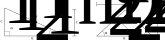
\includegraphics[width=.8\textwidth]{fig/triang.pdf}
\caption{}
\label{fig:tria}
\end{figure}
Consideriamo il caso di una macchina idraulica e vediamo come possiamo trovare il luogo dei punti di funzionamento simili sul piano delle prestazioni e quindi come le curve di prestazioni adimensionali stanno in rapporto con le curve di prestazioni dimensionali.

Se rileviamo le prestazioni di una pompa otteniamo la curva di funzionamento caratteristica (diagramma prevalenza-portata) per un certo valore della velocità di rotazione (figura \ref{fig:hq}).
\begin{figure}[h!]
\centering
  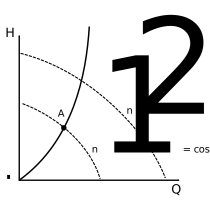
\includegraphics[width=.3\textwidth]{fig/hq.pdf}
\caption{}
\label{fig:hq}
\end{figure}
Queste sono curve espresse in funzione di grandezze dimensionali, ma andando ad adimensionalizzare si possono ottenere tali curve in funzione delle relative cifre di pressione e di flusso.  Si consideri un punto di funzionamento $A$, il luogo dei punti di funzionamento simili ad $A$ sarà caratterizzato dal fatto di avere stessi $\varphi$ e $\psi$.

Considerando quindi il generico punto $x$ posso scrivere
\begin{equation}
\varphi = \frac{Q}{w D^3}= \frac{Q_x}{w_x D^3}
\end{equation}
Considerando una macchina con lo stesso diametro posso scrivere
\begin{equation}
\frac{Q_x}{Q}=\frac{w_x}{w} \; \Rightarrow \; Q_x = Q \frac{w_x}{w}
\end{equation}
Imponendo invece l'uguaglianza della cifra di pressione
\begin{equation}
\psi = \frac{gH}{w^2 D^2}= \frac{gH_x}{w_x^2 D^2}
\end{equation}
In questo modo si ottiene
\begin{equation}
H_x = H(\frac{w_x}{w})^2 = H(\frac{Q_x}{Q})^2 \Rightarrow H_x = \frac{H}{Q^2}Q_x^2
\end{equation}
Che è l'equazione di una parabola sul piano H-Q, passante per il punto A e per l'origine degli assi. 
Noto che il lavoro varia al variare del quadrato della velocità angolare mentre la portata varia linearmente. 
Ad ogni curva $\varphi - \psi$ corrisponde una curva di rendimento, posso quindi individuare una coppia $\bar{\varphi} - \bar{\psi}$ ottimale (figura \ref{fig:adim}).
\begin{figure}[h!]
\centering
  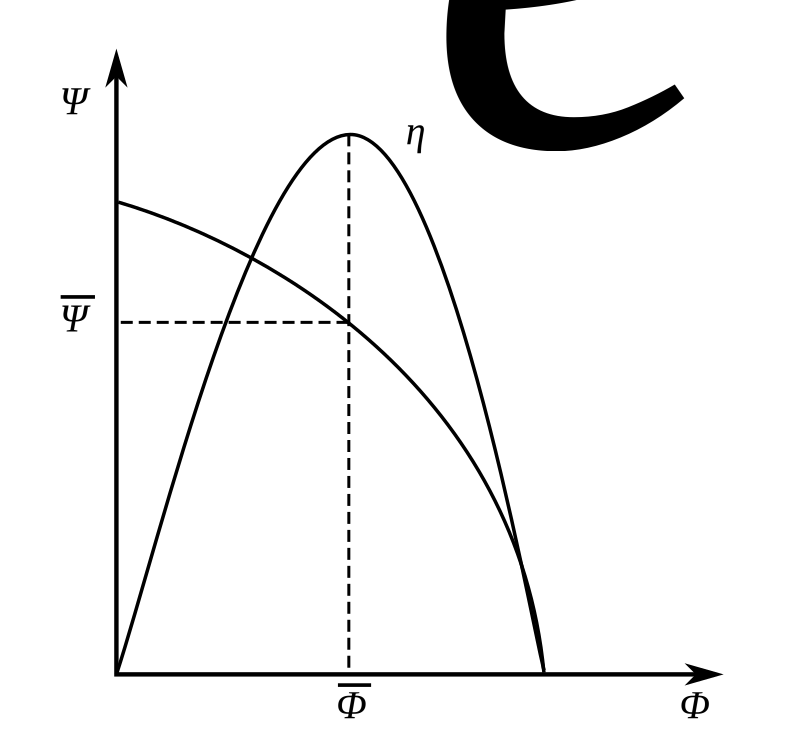
\includegraphics[width=.3\textwidth]{fig/adim.pdf}
\caption{}
\label{fig:adim}
\end{figure}
Posso anche definire il coefficiente di velocità periferica.
\begin{equation}
k_P = \frac{w D}{\sqrt{L_i}}
\end{equation}
Si tratta di una cifra che lega la velocità periferica della macchina al lavoro ideale della stessa.

Quando ho $\varphi$ e $\psi$ posso definire una cifra di potenza adimensionalizzata come prodotto delle due.
\begin{equation}
\Lambda = \frac{P_e}{\rho w^3 D^5}
\end{equation}
Per macchina motrice
\begin{equation}
\Lambda = \varphi \psi \eta_e
\end{equation}
Per macchina operatrice
\begin{equation}
\Lambda = \frac{\varphi \psi}{\eta_e}
\end{equation}
Con la seguente espressione posso poi eliminare la caratteristica geometrica ottenere il numero specifico di macchina (o velocità specifica) che rappresenta una condizione di funzionamento lavoro-portata indipendente dalla dimensione della macchina. 
\begin{equation}
w_s = k = \varphi^{1/2} \psi^{-3/4} = w \frac{\sqrt{Q}}{L_i^{3/4}}
\end{equation}
<<<<<<< Updated upstream
La forma della macchina varierà al variare di k . Avere dei k piccoli significa avere delle macchine nelle quali il termine di scambio di energia è prevalente rispetto al termine di portata. Questo numero permette, grazie all'esperienza storica (ovvero di tutti i dati che il progettista o la sua azienda possiedono in merito alle prestazioni di altre macchine), di classificare la forma geometrica di una macchina in base alle condizioni portata - lavoro.
=======
La forma della macchina varierà al variare di k . Avere dei k piccoli significa avere delle macchine nelle quali il termine di scambio di energia è prevalente rispetto al termine di portata. Questo numero permette, grazie all’esperienza storica (ovvero di tutti i dati che il progettista o la sua azienda possiedono in merito alle prestazioni di altre macchine), di classificare la forma geometrica di una macchina in base alle condizioni portata - lavoro.
>>>>>>> Stashed changes
\begin{figure}[h!]
\centering
  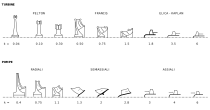
\includegraphics[width=\textwidth]{fig/numcar.pdf}
\caption{Variazione della forma delle giranti delle turbine idrauliche al variare del numero caratteristico di macchina.}
\label{fig:numcar}
\end{figure}
Queste cifre sono funzioni di k. Possono allora essere definite delle curve che riportano in ascissa il valore del numero caratteristico k e sulle ordinate i valori dei 4 rapporti.
Sfruttando l'esperienza possiamo analizzare le migliori macchine esistenti e vedere
quanto valgono per quelle macchine le cifre adimensionali $\pi_i$ , $\pi_j$ e diagrammarle in funzione di k . Facciamo un esempio concreto considerando una tipica macchina radiale (una pompa centrifuga) e consideriamo la sezione meridiana semplificata al massimo (figura \ref{fig:pala}).
\begin{figure}
\centering
\begin{minipage}{.5\textwidth}
  \centering
  \includegraphics[width=.9\linewidth]{fig/pala.pdf}
  \captionof{figure}{}
  \label{fig:pala}
\end{minipage}%
\begin{minipage}{.5\textwidth}
  \centering
  \includegraphics[width=.6\linewidth]{fig/primo_1.pdf}
  \captionof{figure}{}
  \label{fig:primo_1}
\end{minipage}
\end{figure}
Si definiscono le seguenti dimensioni caratteristiche più significative. Si tratta di un esempio didattico, in realtà posso andare a definire un database molto più ampio e raffinato. Siano
\begin{itemize}
\item[-]$D_2$: diametro massimo della girante;\\
\item[-]$D_1$: diametro massimo della sezione di ingresso;\\
\item[-]$D_1^{'}$: diametro minimo della sezione d'ingresso;\\
\item[-]$b_2$: altezza della pala in uscita;\\
\item[-]$b_1$: altezza della pala in ingresso.
\end{itemize}
Per definire $b_1$ bisogna prendere il diametro medio e con riferimento al punto di intersezione tra questo ed il profilo della pala in ingresso si traccia la circonferenza inscrivibile nella sezione d’ingresso. Come grandezza caratteristica della sezione d’ingresso prendo proprio il diametro di questa circonferenza.
Per queste grandezze posso definire le seguenti cifre adimensionali:
\begin{align*}
\frac{D_1}{D_2} \; \; \; \frac{D_1^{'}}{D_2} \; \; \; \frac{b_1}{D_2} \; \; \; \frac{b_2}{D_2} 
\end{align*}
Queste cifre sono funzioni di $k$. Posso allora essere definite delle curve che riportano in ascisse il valore del numero caratteristico $k$ ed in ordinate i valori dei 4 parametri.
Naturalmente fissato $k$ devo poi determinare il numero di giri a cui deve lavorare la macchina. 
Ricapitolando, note portata, prevalenza e fissata la velocità di rotazione, conosco il valore di $k$. Entrando in questi diagrammi si trovano i valori dei quattro parametri e quindi definisco per sommi capi la sezione meridiana della nostra macchina (figura \ref{fig:primo_1}).

Esiste una dimensione ottimale cioè una dimensione alla quale corrisponde il massimo rendimento. Bisogna però definire un’ulteriore grandezza detta diametro specifico.
\begin{equation}
D_s= \varphi^{-1/2} \psi^{1/4} = D \cdot \frac{L_i^{1/4}}{\sqrt{Q}}
\end{equation}
Bisogna cercare di eliminare la velocità di rotazione. È stato verificato che esiste, con riferimento alle dimensioni di massimo rendimento, un legame tra $D_s$ e $w_s$. 
\begin{equation}
D_s=f(w_s)
\end{equation}
Questa funzione è descritta empiricamente sul \textit{Diagramma di Cordier}. Questo diagramma rappresenta l’interpolazione di una serie di dati sperimentali (da vedere come correlazione statistica).
Grazie alle curve di Balié è possibile osservare l’entità delle variazioni che si ottengono andando a discostarsi, entro certi limiti, dalla curva di Cordier.
Si può estendere questa relazione con i diagrammi di Baliè, intorno alla curva si disegnano curve di isorendimento.
\begin{figure}
\centering
\begin{minipage}{.5\textwidth}
  \centering
  \includegraphics[width=.95\linewidth]{fig/cord_diag.pdf}
  \captionof{figure}{Diagramma di Cordier}
  \label{fig:cord_diag}
\end{minipage}%
\begin{minipage}{.5\textwidth}
  \centering
  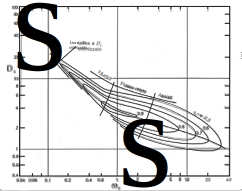
\includegraphics[width=.95\linewidth]{fig/primo_3.pdf}
  \captionof{figure}{}
  \label{fig:primo_3}
\end{minipage}
\end{figure}

\section{Influenza di Re}
Queste considerazioni sono state fatte trascurando l'influenza di Re. Ricordando il diagramma di Moody la relazione è fatta rispetto a $\epsilon/D$. Per le macchine è essenzialmente uguale, al diminuire di Re le curve si spostano più in basso, questo effetto si riflette in un abbassamento di rendimento e quindi di prevalenza.

Questo è un fenomeno prevedibile in termini statistici, storicamente grazie all'accumulazione di dati sono stati definiti due fattori di correzione, di rendimento $f_\eta$ e $f_\psi$ diagrammati rispetto a $Re$. Man mano che $Re$ scende il loro effetto diventa sempre più importante. 
\begin{figure}
\centering
\begin{minipage}{.4\textwidth}
  \centering
  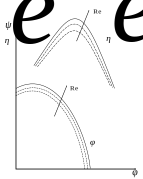
\includegraphics[width=.95\linewidth]{fig/secondo_1.pdf}
  \captionof{figure}{}
  \label{fig:secondo_1}
\end{minipage}%
\begin{minipage}{.6\textwidth}
  \centering
  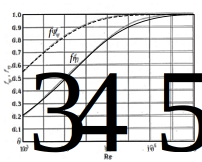
\includegraphics[width=.95\linewidth]{fig/secondo_2.pdf}
  \captionof{figure}{}
  \label{fig:secondo_2}
\end{minipage}
\end{figure}

Parto dalla $w_s$, scrivo $\varphi$ e $\psi$ nei diversi punti di funzionamento della macchina in funzione di $w_s$ ($\equiv k$). 
\begin{align*}
w_s= \varphi^{1/2}\psi^{-3/4} \Rightarrow 
\begin{cases}
\psi = \psi(w_s)\\
\eta = \eta(w_s)
\end{cases}
\Rightarrow
\begin{cases}
f_{\psi} = f(Re)\\
f_{\eta} = f(Re)
\end{cases}
\end{align*}
Con i coefficienti correttivi vado a trovare le cifre adimensionali corrette \begin{align*}
\begin{cases}
\psi_{corretto} = f_{\psi} \cdot \psi(w_s)\\
\eta_{corretto} = f_{\eta} \cdot \eta(w_s)
\end{cases}
\end{align*}
A questo punto è possibile procedere a ritroso. Trovato il valore corretto avrò
\begin{align*}
\omega_s = \varphi^{1/2} \psi^{-3/4} =  \varphi_{corretto}^{1/2} \psi_{corretto}^{-3/4} = cost
\end{align*}
partendo proprio dalla definizione di $\omega_s$ è possibile costruire le curve di prestazione corrette.

\section{Effetto scala}
Si considera poi un effetto scala non solo legato alle rugosità superficiali ma anche legato ai giochi. L'effetto scala può essere espresso rispetto ai rapporti dimensionali. Queste relazioni sono sempre costruite per via empirica sulla base dei dati storici.

A parità di bontà di progettazione, geometria, ecc... la macchina grande ha un rendimento maggiore rispetto alla macchina piccola. Questo si spiega facendo due osservazioni: a parità di tecnologia produttiva è possibile ritenere costante il valore della rugosità superficiale delle palettature della girante. In una macchina grande la rugosità relativa sarà quindi più bassa, quindi le perdite di carico saranno superiori nella macchina piccola. In secondo luogo bisogna tener conto dei giochi presenti tra parte fissa e parte mobile, che non possono scendere al di sotto di un certo limite. Nelle macchine grandi questi diventeranno trascurabili. 
\begin{figure}
\centering
  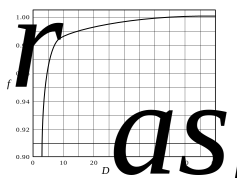
\includegraphics[width=.5\textwidth]{fig/dDchart.pdf}
\caption{}
\label{fig:dDchart}
\end{figure}

Facendo riferimento alle pompe possiamo definire un rapporto dimensionale 
\begin{align*}
\frac{D_1}{D_2} \triangleq  \mbox{Rapporto di scala}, \; D_1 < D_2
\end{align*}
In riferimento alla figura \ref{fig:dDchart} rendimento si può esprimere come
\begin{align*}
\eta = \eta_S \cdot f_r(D)
\end{align*}
E la relazione tra il rendimento tra le pompe di scala diversa è il seguente
\begin{equation}
\frac{1-\eta_1}{1-\eta_2} = \left( \frac{D_2}{D_1}\right)^\alpha
\end{equation}
La stessa operazione viene fatta per le turbine idrauliche
\begin{align*}
\frac{1-\eta_1}{1-\eta_2} = \left[ \frac{Re_{u,2}}{Re_{u,1}} \right]^n, \; \; n=0.1 \div 0.25
\end{align*}
\begin{align*}
\frac{1-\eta_1}{1-\eta_2} =0.5 + 0.5 \left[ \frac{Re_{u,2}}{Re_{u,1}} \right]^{0.2}
\end{align*}
\begin{align*}
\frac{1-\eta_1}{1-\eta_2} = 0.3 + 0.7 \left[ \frac{Re_{u,2}}{Re_{u,1}} \right]^{0.2} \; \to \; \mbox{Turbine Kaplan}
\end{align*}
\section{Flusso comprimibile}
Se si considera il flusso comprimibile le relazioni diventano più complesse. Infatti si ha:
\begin{equation}
\psi=f(\varphi,Ma)
\end{equation}
$\psi$ dipende quindi anche dal numero di Mach. 
Nel diagramma $\varphi-\psi$ si ottengono diverse curve al variare del numero di Mach (Figura \ref{fig:ComprMach}), le curve diventano di difficile lettura e comprensione.Infatti, per diversi valori delle grandezze termodinamiche di temperatura e pressione risulta possibile ottenere le stesse quantità di lavoro unitario, e ciò comporta una mancata definizione univoca dello stesso. Si tratta di una rappresentazione poco fisica e di un esercizio esclusivamente accademico.
\begin{figure}[h!]
\centering
  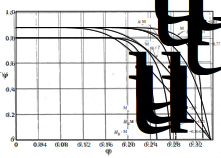
\includegraphics[width=.85\textwidth]{fig/ComprMach.pdf}
\caption{Curve adimensionali di funzionamento di una famiglia di compressori, per un fluido assegnato, a diversi numeri di Mach periferici. Sono definiti $Ma = \frac{w \frac{D}{2}}{a_{01}}$, $Mu = \frac{w \frac{D}{2}}{a}$}
\label{fig:ComprMach}
\end{figure}
Per questo tipo di macchine si utilizzeranno curve molto diverse. Per avere una grandezza confrontabile di funzionamento devo effettuare tutte le prove in condizioni standard. In questo modo posso rappresentare condizioni di funzionamento in modo univoco. 
Definisco il significato dei pedici:
\begin{itemize}
\item $s$: grandezze relative alle condizioni standard;
\item $c$: valori corretti, cioè riportati alle condizioni standard;
\item ``  ": valori da correggere rilevati nel corso della prova.
\end{itemize}
Si elencano di un gas generico miscela di due gas con massa molare $M$\footnote{Nota bene: solo in questo contesto si utilizza $M$ per indicare la massa molare, in tutto il resto del libro viene usato per indicare il numero di Mach}
\begin{align*}
\frac{p}{\rho} = \frac{p_1}{\rho} + \frac{p_2}{\rho} = x_1  \frac{p_1}{\rho_1} + x_2  \frac{p_2}{\rho_2} = RT \left( \frac{x_1}{M_1} + \frac{x_2}{M_2} \right) = RT(\frac{1}{M_{tot}})
\end{align*}
\begin{align*}
c_p = x_1 c_{p1} + x_2 c_{p2}
\end{align*}
\begin{align*}
\cfrac{\gamma}{\gamma -1} = \cfrac{\cfrac{x_1}{M_1} \cfrac{\gamma_1}{\gamma_1 -1}+\cfrac{x_2}{M_2} \cfrac{\gamma_2}{\gamma_2 -1}}{\cfrac{x_1}{M_1}+\cfrac{x_2}{M_2}}
\end{align*}
Con $M_{1,2,tot}$ numero di moli, $x_{1,2}$ frazione molare e $R$ costante dei gas perfetti. Si ricorda poi che definiti calore specifico a pressione costante $c_p$ e calore specifico a volume costante $c_v$ si ha
\begin{align*}
\gamma = \frac{c_p}{c_v}, \;\;\; R = c_p - c_v
\end{align*}

Di seguito vengono riportate le grandezze significative corrette rispetto alle condizioni standard.\\
Rapporto di compressione corretto rispetto alle condizioni ambientali standard:
\begin{align*}
\frac{p_{02}}{p_{01}} = \frac{p_{01c}}{p_{01s}} \; \Rightarrow \; p_{02c} = p_{02}\frac{p_{01s}}{p_{01}}
\end{align*}
Parametro di portata
\begin{align*}
\frac{\dot{m}\sqrt{T_{01}}}{p_{01}}=\frac{\dot{m_c}\sqrt{T_{01s}}}{p_{01s}} \; \Rightarrow \; \dot{m_c} = \dot{m} \sqrt{\frac{T_{01}}{T_{01s}}} \bigg(\frac{p_{01s}}{p_{01}} \bigg)
\end{align*}
Parametro di velocità
\begin{align*}
\frac{n}{\sqrt{T_{01}}}=\frac{n_c}{\sqrt{T_{01s}}} \; \Rightarrow \; n_c = n \sqrt{\frac{T_{01s}}{T_{01}}}
\end{align*}
Si definiscono quindi le condizioni ambientali standard.
Pressione ridotta
\begin{align*}
\delta = \frac{p_{01}}{p_{01s}}
\end{align*}
Temperatura ridotta
\begin{align*}
\theta = \frac{T_{01}}{T_{01s}}
\end{align*}
Si possono esprimere più sinteticamente le grandezze corrette:
\begin{align*}
p_{01c} = \frac{p_{02}}{\delta}
\end{align*}
\begin{align*}
\dot{m_c}= \dot{m} \frac{\sqrt{\theta}}{\delta}
\end{align*}
\begin{align*}
n_c = \frac{n}{\sqrt{\theta}}
\end{align*}
\begin{figure}
\centering
  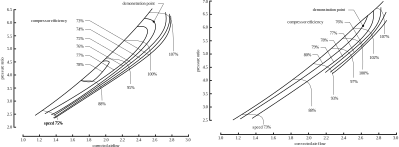
\includegraphics[width=\textwidth]{fig/CompMaps.pdf}
\caption{}
\label{}
\end{figure}
Si ottiene così la portata di massa corretta e il numero di giri corretto.
In questo modo si trovano le mappe di funzionamento delle macchine. Si diagrammano la portata d'aria corretta con il rapporto di compressione. Sono tracciate diverse curve al variare dei giri con le curve di isorendimento.

A questo punto si espande l'espressione di $\varphi$ tenendo conto delle seguenti espressioni di $M_{01}$, $p$ e $a$
\begin{align*}
M_{01}=\frac{w D}{a_{01}}= \frac{w D}{\sqrt{k R T_{01}}}, \;\;\;p = \rho_i RT, \;\;\; a = \sqrt{k R T}
\end{align*}
\begin{equation}
\varphi = \frac{\dot{m}}{\rho_{01} w D^3} = \frac{\dot{m}}{\rho_{01} M_{01} a_{01} D^2} = \frac{\dot{m} R T_{01}}{\rho_{01} M_{01} \sqrt{k R T_{01}} D^2} = \frac{\dot{m} \sqrt{R T_{01}}}{\rho_{01} M_{01} \sqrt{k} D^2}
\end{equation}
Mentre la cifra $\psi$ è esprimibile in funzione dei soli $M_{01}$, rapporto di compressione e delle caratteristiche del fluido ($k$)
\begin{equation}
\psi = \cfrac{L_i}{w^2 D^2} = \cfrac{\Delta h_{0s}}{w^ 2 D^2} = \cfrac{\cfrac{k}{k-1} R T_{01}\left[ \bigg( \cfrac{p_{02}}{p_{01}} \bigg)^{\frac{k-1}{k}}-1\right]}{M_{01}^2 k R T_{01}} = \cfrac{\cfrac{1}{k-1} \left[ \bigg( \cfrac{p_{02}}{p_{01}} \bigg)^{\frac{k-1}{k}}-1\right]}{M_{01}^2 }
\end{equation}

L'idea è quella di rappresentare in modo univoco il comportamento del compressore usando i termini $\varphi$, $\psi$ ma mantenendo la significatività fisica.

Se utilizzo lo stesso fluido posso trascurare $R$ e $k$. Utilizzando la stessa macchina trascuro anche $D$, riferendosi alle condizioni standard posso considerare $M_{01}=cost$. Sotto le precedenti ipotesi ottengo le seguenti relazioni semplificate:
\begin{align*}
M_{01} \to \frac{w D}{\sqrt{R T_{01}}} \Rightarrow M_{01} \to \frac{w}{\sqrt{T_{01}}}
\end{align*}
\begin{align*}
\varphi \to \frac{\dot{m} \sqrt{RT_{01}}}{\rho_{01} D^2} \Rightarrow \varphi \to \frac{\dot{m} \sqrt{T_{01}}}{\rho_{01}}
\end{align*}
\begin{align*}
\psi \to \frac{p_{02}}{p_{01}}
\end{align*}
Si tratta di grandezze che posso andare a misurare in un banco prova. 
La mappa di funzionamento del compressore assume quindi una forma più leggibile, sull'asse delle ascisse ho la portata in massa corretta con la temperatura in ingresso e sulle ordinate il rapporto di compressione. Assieme a queste posso anche costruire le linee di isorendimento  e quindi la curva ideale operativa del compressore data dall'inviluppo delle curve di isorendimento.
\begin{figure}
\centering
  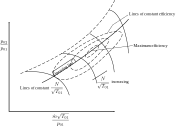
\includegraphics[width=.8\textwidth]{fig/secondo_8.pdf}
\caption{}
\label{fig:secondo_8}
\end{figure}
Guardando al diagramma in figura \ref{fig:secondo_8} si vede che abbiamo un fenomeno noto come ingolfamento del compressore, in particolare si vede dalle linee a velocità costante che tendono a diventare verticali in prossimità delle condizioni di ingolfamento . Intendiamo il raggiungimento di quella condizione di funzionamento in cui non è più possibile variare la portata variando il rapporto delle pressioni attorno alla macchina.
Questo perchè in qualche punto si raggiungono le condizioni di flusso sonico e quindi, ricordando lo studio dell'ugello convergente-divergente, abbiamo un
blocco sonico delle portata.

L'obiettivo è quello di lavorare il più possibile vicino alla ``operating line" che è la zona di massimo rendimento, il problema è che ci si trova pericolosamente vicino alla ``surge line". Oltre la surge line si innesca il fenomeno del pompaggio che può compromettere la macchina e l'impianto irrimediabilmente.

Riassumendo, nel comprimibile, operativamente si descrive il funzionamento delle turbomacchine non rispetto alle cifre di flusso e pressione, bensì attraverso nuove cifre più significative in questo contesto.
\section{Richiamo di termodinamica}
Lo scambio termico è trascurabile per i bassi tempi di residenza del fluido nel condotto, per questo motivo si considera il rotore adiabatico.

In un rotore adiabatico, per il primo principio della termodinamica, essendo il flusso di calore nullo, il lavoro è dato dal salto entalpico tra gli stati $1$ e $2$
\begin{equation}
L_{12}^{'} = h_{t1}-h_{t2}
\end{equation}
\begin{equation}\label{eq:ent_tot}
h_t=h+\frac{c^2}{2}+gz
\end{equation}
Con: 
$h_t$: entalpia totale\\
$h$: entalpia statica\\
$c^2/2$: quota cinetica\\
$gz$: quota gravitazionale\\[2mm]
Per una macchina motrice\footnote{Nel caso delle macchine operatrici si invertono i pedici $1$ e $2$ così da avere lavori per convenzione sempre positivi} si può scrivere
\begin{equation}\label{eq:L12}
L_{12}^{'} = \begin{cases} u_1 c_{u1}-u_2 c_{u2}\\
\cfrac{c_1^2-c_2^2}{2}+\cfrac{u_1^2-u_2^2}{2}-\cfrac{w_1^2-w_2^2}{2} \end{cases}
\end{equation}

Naturalmente il lavoro è stato scritto, in base alle note convenzioni, per una macchina motrice.

Il lavoro è costituito da una parte cinetica e da una parte statica, il che si può osservare confrontando le espressioni di $L_{12}^{'}$ nelle formule \ref{eq:ent_tot} e \ref{eq:L12}, in particolare la quota parte cinetica dipende dalla componente assoluta della velocità ($c$), mentre quella statica dipende dalle componenti assiale ($u$) e relativa ($w$).

Dato che in una macchina puramente assiale si conserva l'omonima componente u della velocità ( $u = cost$ ), allora il contributo $u_1^2 - u_2^2$ nell'espressione del lavoro è nullo: per questo una macchina radiale a parità di numero di stadi e condizioni, elabora più lavoro di una assiale, in quanto $u_1^2 - u_2^2$ è maggiore di zero.

Ponendomi come osservatore relativo rispetto al rotore eguagliando le due espressioni per il lavoro posso scrivere
\begin{equation}
u_1 c_{u1} - u_2 c_{u2} = h_1 + \frac{c_1^2}{2}+gz_1-h_2-\frac{c_2^2}{2}-gz_2
\end{equation}
Posso quindi definire la rotalpia\footnote{Grandezza che rappresenta l'entalpia totale del moto relativo} come grandezza di stato ed è tale, proprio in virtù dell'adiabaticità del rotore, e quindi per la conservazione dell'energia vale:
\begin{equation}
h+\frac{c^2}{2}+gz-u c_u = cost. = I
\end{equation}

Riassumendo:
\begin{itemize}
\item $I=cost.$ in un rotore adiabatico;
\item $h_t=cost.$ in uno statore adiabatico.
\end{itemize}

Posso esprimere tutte le grandezze fin'ora viste in un piano $T-s$ o $h-s$.

\section{Rendimenti per i compressori}
Si riporta la trattazione dei rendimenti fatta per i compressori, i concetti riportati valgono anche per le turbine, cambia solamente le convenzione nei segni. La seguente trattazione è un estratto del libro Macchine a fluido, ISBN 978-88-251-7397-0. 

Il rendimento è definito qualitativamente come il rapporto tra l'effetto utile ed il lavoro svolto dalla macchina. Sul lavoro svolto non ci sono ambiguità mentre in merito all'effetto utile si possono avere diverse formulazioni. Il lavoro utile può essere preso come il salto entalpico associato al rapporto di compressione tra le pressioni statiche o totali ingresso-uscita, oppure come combinazione tra grandezze statiche e totali tra ingresso e uscita. Le diverse definizioni di rendimento sono sostanzialmente da imputare alle quote cinetiche ingresso/uscita che possono essere contate o meno come effetto utile.
\begin{figure}
\centering
  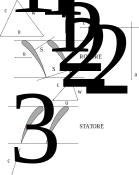
\includegraphics[width=.5\textwidth]{fig/schieraTComp.pdf}
\caption{}
\label{fig:schieraTComp}
\end{figure}
Con riferimento alla trasformazione termodinamica, trascurando i contributi cinetici all'ingresso e all'uscita, si possono definire il rendimento adiabatico ed il rendimento politropico. Tale approccio è spesso utilizzato quando non si vuole entrare nel dettaglio della macchina come invece è necessario fare quando si vogliono studiare le prestazioni dei singoli stadi. 

Nel caso di rendimento adiabatico, definendo con $l_{is}$ il lavoro lungo la trasformazione isoentropica e con $l_r$ quello lungo l'adiabatica reale e facendo riferimento alla \ref{fig:Rend1}, la definizione diventa
\begin{align*}
\eta_{ad} = \frac{h_{2'} - h_1}{h_2 - h_1} = \frac{c_p \left( T_{2'} - T_1 \right)}{c_p \left( T_2 - T_1 \right)} = \frac{\left( \beta^{\cfrac{\gamma -1}{\gamma}} -1 \right)}{\left( \beta^{\cfrac{n -1}{n}} -1 \right)} = \frac{l_{is}}{l_r}
\end{align*}
Avendo assunto $c_p = cost$ con la temperatura e pressione, ed essendo $\gamma$ l'indice dell'isoentropica ed $n$ quello della politropica corrispondente alla trasformazione reale. La scelta di questa definizione, oltre al facile utilizzo, è quella di fornire una indicazione diretta dello scostamento della trasformazione da quella migliore possibile che è l'isoentropica, senza dedicare particolare attenzione alle energie cinetiche presenti all'interno del sistema macchina.
\begin{figure}
\centering
\begin{minipage}{.45\textwidth}
  \centering
  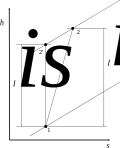
\includegraphics[width=.9\linewidth]{fig/Rend1.pdf}
  \captionof{figure}{}
  \label{fig:Rend1}
\end{minipage}%
\begin{minipage}{.55\textwidth}
  \centering
  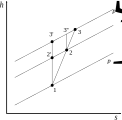
\includegraphics[width=.9\linewidth]{fig/Rend2.pdf}
  \captionof{figure}{}
  \label{fig:Rend2}
\end{minipage}
\end{figure}
Un'altra applicazione è il rendimento politropico che assume la trasformazione politropica reversibile tra i punti $1$ e $2$ come riferimento per la trasformazione reale. Tale assunzione viene incontro alla necessità, nel caso di macchine multistadio - o a singolo stadio ma con elevato rapporto di compressione - di non imputare ad una porzione di trasformazione la storia dei volumi specifici precedenti ed in particolar modo le irreversibilità precedenti. Con riferimento alla \ref{fig:Rend2}, dividendo la trasformazione in 3 porzioni, l'ultima parte della compressione richiede un salto entalpico pari a $\Delta h_r = h_3 - h_2$ che può essere confrontato con $\Delta h_{is} = h_{3'} - h_{2'}$ oppure con $\Delta h_is = h_{3''} - h_2$ a seconda dell'analisi che si vuole compiere sulla macchina.

Qualora si voglia analizzare il singolo stadio, o la singola porzione di trasformazione, allora appare corretto confrontare il salto reale con quello tra i punti $3''$ e $2$ in quanto più attinente alla trasformazione reale oggetto dell'attenzione. A causa della divergenza delle isobare il salto entalpico $3''$ e $2$ risulta maggiore di quello $3'$ e $2'$, dando luogo ad un rendimento maggiore. Se tale ragionamento viene esteso a porzioni infinitesime di compressione ci si avvicina alla definizione di rendimento politropico.

La scelta della trasformazione politropica reversibile - che tiene conto al suo interno di un riscaldamento del fluido operato da una sorgente esterna ma equivalente a quello causato dalle irreversibilità - consente di evidenziare il solo contributo delle irreversibilità e cioè del termine $\int Tds$.

Considerata allora la trasformazione 1-2, chiamato $l_p$ il lavoro lungo la politropica reversibile e $l_r$ il lavoro lungo la trasformazione adiabatica reale, il rendimento assume la seguente forma
%\begin{align*}
%\eta_p = \frac{l_p}{l_r} = \frac{\frac{nRT_1}{n-1} \left[ \left( \frac{p_2}{p_1} \right)^{\frac{n-1}{n} -1 \right]}{\frac{ \gamma RT_1}{\gamma-1} \left[ \left( \frac{p_2}{p_1} \right)^{\frac{n-1}{n} -1 \right]} = \frac{n}{\gamma} \frac{\gamma -1}{n -1}
%\end{align*}
Confrontando i due rendimenti a pari rapporto di compressione si vede come la differenza tra rendimento politropico e adiabatico aumenti al crescere del rapporto di compressione e che il rendimento adiabatico è sempre minore del politropico.
\begin{figure}
\centering
\begin{minipage}{.45\textwidth}
  \centering
  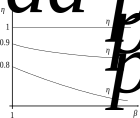
\includegraphics[width=.9\linewidth]{fig/Rend3.pdf}
  \captionof{figure}{}
  \label{fig:Rend3}
\end{minipage}%
\begin{minipage}{.55\textwidth}
  \centering
  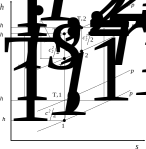
\includegraphics[width=.9\linewidth]{fig/Rend4.pdf}
  \captionof{figure}{}
  \label{fig:Rend4}
\end{minipage}
\end{figure}
Infatti poichè $\eta_p = l_p / l_r$ e $\eta_{ad} = l_{is} / l_r$, si ottiene
\begin{align*}
\eta_{ad} = \eta_p \frac{l_is}{l_r} = \eta_p \frac{\frac{\gamma}{\gamma-1} \left(\beta^{\frac{\gamma -1}{\gamma}}-1 \right)}{\frac{n}{n-1} \left(\beta^{\frac{n -1}{n}}-1 \right)}
\end{align*}
ed essendo $l_p$> $l_{is}$ si ottiene $\eta_{ad} < \eta_p$. Al fine di evidenziare al differenza tra le due trasformazioni è possibile definire il lavoro di controrecupero definito come
\begin{align*}
f = \frac{l_p - l_{is}}{l_{is}} = \frac{l_p}{l_{is}} -1 = \eta_p \frac{\left( \beta^{\frac{n-1}{n}} -1 \right)}{\left( \beta^{\frac{\gamma-1}{\gamma}} -1 \right)} -1 = \frac{\eta_p}{\eta_{ad}} -1
\end{align*}
Al crescere della differenza tra i due rendimenti, il fattore di controrecupero aumenta. Tale fattore è sempre maggiore di zero e si annulla quando i due rendimenti sono uguali, cioè quando non ci sono effetti termici sulla densità come avviene per le macchine idrauliche.

Qualora si voglia studiare gli effetti delle quote cinetiche, è possibile definire diversi tipi di rendimento, sempre definiti nella scia del rendimento adiabatico, denominati "total to total" e "total to static". Con riferimento alla \ref{fig:Rend4} si definiscono
\begin{itemize}
\item Rendimento total to total
\begin{align*}
\eta_{T,T} = \frac{\Delta h_{T,is}}{\Delta h_T} = \frac{h_{T,2'} - h_{T,1}}{h_{T,2} - h_{T,1}} = \frac{h_{2'} - h_1 + \left( \frac{c_2^2 - c_1^2}{2} \right)}{h_2 - h_1 + \left( \frac{c_2^2 - c_1^2}{2} \right)} = \frac{h_{2'} - h_1 + \left( \frac{c_2^2 - c_1^2}{2} \right)}{l_r} = \frac{l_{is}}{l_r}
\end{align*}
\item Rentimento Total to Static
\begin{align*}
\eta_{T,S} = \frac{h_{2'} - h_{T,1}}{h_{T,2} - h_{T,1}} = \frac{h_{2'} - h_1 - \left( \frac{ c_1^2}{2} \right)}{h_2 - h_1 + \left( \frac{c_2^2 - c_1^2}{2} \right)} = \frac{h_{2'} - h_1 + \left( \frac{c_2^2 - c_1^2}{2} \right)}{l_r} = \frac{l_{is}}{l_r}
\end{align*}
\end{itemize}
\pagebreak


\chapter{Turbomacchine assiali - Generalità}
\footnote{Questo paragrafo è stato estratto dagli appunti di Caizzi.} Nel corso di Macchine le macchine sono state studiate sulla base di una teoria che possiamo definire monodimensionale, come se ci fosse un flusso privo di caratteristiche bi o tridimensionali, quindi immaginando che tutti i piani meridiani siano uguali a se stessi e trascurando quanto avviene in direzione radiale. Quest'analisi monodimensionale è uno strumento utilissimo che consente di capire come funziona una macchina e come si può procedere al dimensionamento di massima. Per procedere oltre nel dimensionamento e nella verifica delle prestazioni, si passa da un approccio monodimensionale ad un approccio bidimensionale.\\
L’approccio bidimensionale sarà ancora approssimato perché il flusso per una turbomacchina è tridimensionale; questa approssimazione però si avvicina maggiormente alla realtà. Quest'analisi bidimensionale potrebbe essere applicata a qualsiasi tipo di macchina ma trova applicazione particolarmente utile proprio nel caso di macchine assiali.

Per capire in cosa consiste questo approccio si considera la figura \ref{fig:ReticoloComp1}.
\begin{figure}
\centering
  \includegraphics[width=.8\textwidth]{fig/ReticoloComp.pdf}
\caption{Reticolo di calcolo quasi-3D per una sezione di un compressore assiale bistadio}
\label{fig:ReticoloComp1}
\end{figure}
\'E possibile applicare un’analisi di tipo bidimensionale per esempio alla coppia $ROTORE\;2 - STATORE\;2$ in cui lo sviluppo della macchina è quasi perfettamente assiale. Si immagini che le linee di corrente siano parallele all'asse di rotazione e che tutte le sezioni meridiane siano uguali a se stesse, ossia si supponga che le linee di corrente siano assialsimmetriche; nello studio della macchina quindi, si studiano separatamente le due sezioni.\\
Si prenda una linea di corrente e si sezioni la macchina lungo la superficie cilindrica di questa linea. Questa superficie cilindrica andrà a sezionare tutte le pale in corrispondenza dello stesso valore di raggio. Immaginando di prendere la superficie cilindrica, tagliandola lungo una generatrice e stendendola sul piano si ottiene la stella di pale in una schiera piana di pale.\\
Poi lo studio è completato con lo studio del piano meridiano dove si andrà a vedere come cambiano le condizioni del flusso al variare del raggio. Quest'analisi verrà fatta in corrispondenza dei punti contenuti in delle sezioni comprese tra una pala e l’altra.\\
Le linee verticali sono linee che è possibile sempre individuare e che non intersecano le pale; in corrispondenza di queste sezioni ortogonali vengono calcolate le condizioni di equilibrio radiale del flusso. Bisogna sempre supporre di avere l'assialsimmetria. Valutando delle sezioni che intersecano la pala ci sarà un flusso periodico e quindi bisogna considerare delle forze scambiate tra fluido e pala. Quindi i due punti fondamentali dell'analisi bidimensionale sono:
\begin{itemize}
\item studio della schiera di pale;
\item studio dell'equilibrio radiale.
\end{itemize}
Unendo i risultati di questi due studi si ottiene il comportamento della macchina (abbastanza simile a quello reale).
Con l’approccio bidimensionale si trascura il fatto che la linea di corrente non è perfettamente assiale (abbiamo una componente radiale) e si vede che nella sezione studiata il flusso non è perfettamente assialsimmetrico.\\
Tutto quello che sfugge a questa analisi costituisce una serie di strutture di flusso definite flussi secondari che sono funzione del modo in cui sono stati modellizzati i flussi principali.
\section{Nomenclatura}
\begin{figure}[h!]
\centering
\begin{minipage}{.5\textwidth}
  \centering
  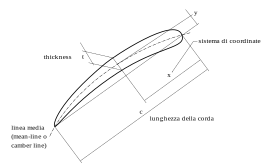
\includegraphics[width=\linewidth]{fig/profiloDef.pdf}
  \captionof{figure}{}
  \label{fig:profiloDef}
\end{minipage}
\begin{minipage}{.48\textwidth}
  \centering
  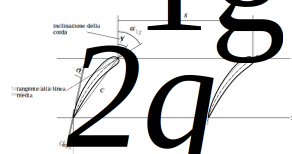
\includegraphics[width=.98\linewidth]{fig/schiera_2.pdf}
  \captionof{figure}{}
  \label{fig:schiera_2}
\end{minipage}
\end{figure}
Analizzando la figura \ref{fig:profiloDef}, per il profilo isolato si definiscono le seguenti grandezze adimensionali:
\begin{align*}
\cfrac{x}{c} \;\;\;\;\;\; \cfrac{y}{c} \;\;\;\;\;\; \cfrac{t}{c}
\end{align*}
con:\\[1mm]
$t$: spessore massimo del profilo isolato;\\
$c$: lunghezza della corda;\\
$x,y$: coordinate.\\[2mm]
Quanto detto per il profilo isolato varrà anche per i profili in schiera. Come è lecito pensare, nelle applicazioni meccaniche non si limiterà ad una sola pala, ma si considereranno macchine che necessitano di più pale per assolvere al proprio compito. Si definisce quindi la solidità della schiera come
\begin{equation}
\sigma = \cfrac{c}{s}
\end{equation}
con $s$ distanza tra due punti omologhi di due pale successive.
\subsection{Definizioni geometriche}
Analizzando la figura \ref{fig:schiera_2} si definiscono:\\[1mm]
$\alpha_{1g}, \alpha_{2g}$ \footnote{Il pedice "g" sta per geometrico}: inclinazioni delle tangenti alla linea media rispetto alla direzione ortogonale;\\
$\theta$: deflessione geometrica del profilo, differenza tra angolo in ingresso e in uscita (angolo di camber). $\theta = \alpha_{1g} - \alpha_{2g} = \Delta \alpha_{g}$;\\
$\gamma$: angolo di calettamento del profilo della schiera, inclinazione della corda rispetto alla direzione ortogonale.\\
\subsection{Definizioni per la corrente fluida}
Si immagina poi di investire la schiera di pale con una corrente fluida dotata di un certo angolo di incidenza. Si ricavano quindi i seguenti parametri (figura \ref{fig:palasing}):\\[1mm]
$\alpha_i$: inclinazione del vettore velocità rispetto alla direzione di riferimento ortogonale alla schiera. Una palettatura non riuscirà mai a deviare la corrente tanto quanto è inclinata geometricamente;\\
$\alpha$: angolo di attacco del flusso rispetto la schiera, inclinazione del vettore velocità in ingresso con riferimento alla corda;\\
$i$: angolo di incidenza, inclinazione del vettore velocità in ingresso rispetto la tangente alla linea media;\\
$\delta$: angolo di deviazione o deviazione, inclinazione del vettore velocità in uscita rispetto la tangente alla linea media;\\
$\epsilon = \Delta \alpha$: entità della deflessione subita dal flusso tra ingresso e uscita.\\[2mm]
\begin{figure}
\centering
  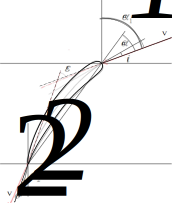
\includegraphics[width=.45\textwidth]{fig/palasing.pdf}
\caption{}
\label{fig:palasing}
\end{figure}
\\Dalle considerazioni geometriche viste prima si può infine scrivere:
\begin{align*}
\varepsilon = \theta + i - \delta
\end{align*}
Nel caso delle turbine le deviazioni sono più alte rispetto ai compressori visto che rallentare una corrente è sempre molto più facile che accelerarla.
\subsection{Forze}
Si possono scrivere le forze agenti sulla schiera di pale rispetto al sistema di riferimento assiale - tangenziale per determinare la coppia, ovvero la potenza fornita all'albero nel caso di compressore. La componente assiale sarà la spinta che i cuscinetti dovranno sopportare per il funzionamento e si ripercuote anche sulle perdite di carico.\\
Le stesse forze, poste in un sistema di riferimento diverso (vedi figura \ref{fig:LDref}), sono comunemente note come portanza (Lift) e resistenza (Drag).\\
\begin{align*}
	\begin{cases}
		F_a = f(\Delta v, \Delta p_0)\\
		F_t = f(\Delta v, \Delta p_0)
	\end{cases} \hspace{2cm}
	\begin{cases}
	L = f(F_a,F_t)\\
	D = f(F_a,F_t)
	\end{cases}
\end{align*}
Si consideri ora una schiera palare e un volume di controllo ($ABCD$, di lato minore $AB=s$) che segue la linea media del profilo, figura \ref{fig:schiera1}. Le velocità in ingresso e in uscita vengono scomposte nella direzione assiale e tangenziale. 
\begin{figure}
\centering
\begin{minipage}{.4\textwidth}
  \centering
  \includegraphics[width=.95\linewidth]{fig/schiera1.pdf}
  \captionof{figure}{}
  \label{fig:schiera1}
\end{minipage}%
\begin{minipage}{.6\textwidth}
  \centering
  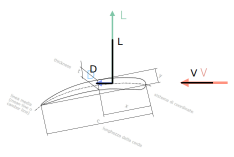
\includegraphics[width=.85\linewidth]{fig/LDref.pdf}
  \captionof{figure}{}
  \label{fig:LDref}
\end{minipage}
\end{figure}
\\Applicando l'equazione di conservazione della portata in massa (equazione di continuità) si ha:
\begin{equation}
s \rho V_{1a} = s \rho V_{2a} \;\;\;\; \Rightarrow \;\;\;\; V_{1a} = V_{2a} = V_a
\end{equation}
dove si è ipotizzato $\rho$ costante, in quanto per un compressore assiale i rapporti di compressione per stadio sono modesti (nel caso di una turbina non sarebbe valido).\\
Per quanto riguarda la conservazione della quantità di moto, vale in direzione tangenziale:
\begin{align*}
F_t= \dot{m} \cdot \Delta V_t = s \rho	V_a \cdot (V_{1t}-V_{2t})
\end{align*}
e in direzione assiale:
\begin{align*}
F_a = s \cdot (p_1 - p_2)
\end{align*}
Scrivendo la pressione nelle componenti di pressione statica e dinamica si espande l'espressione per le forze assiali ottenendo:
\begin{align*}
F_a = s \cdot ( p_1 - p_2) &= s \cdot \left( p_{01} - \frac{1}{2} \rho V_1^2 - p_{02} + \frac{1}{2} \rho V_2^2 \right)\\
&= \frac{1}{2} \rho s \left( V_2^2 - V_1^2 \right) + s \left( p_{01} - p_{02} \right)\\
&= \frac{1}{2} \rho s \left( V_{t2}^2 + \cancel{V_a^2} - V_{t1}^2- \cancel{V_a^2} \right) + s \Delta p_0\\
&=\cfrac{1}{2} \rho s (V_{t2}-V_{t1}) (V_{t2}+V_{t1}) + s \Delta p_0
\end{align*}
con:\\[1mm]
$\Delta p_0$: perdita di pressione totale, rappresenta quindi la perdita di carico nel deflusso attraverso la schiera; \\
$(V_{t2}-V_{t1})$ rappresenta il trasferimento di quantità di moto. \\[2mm]
Dividendo il termine $(V_{t2}+V_{t1})$ per $2$ si ottiene l'espressione della velocità tangenziale all'infinito, ossia la velocità media indisturbata:
\begin{align*}
V_{t \infty}=\cfrac{(V_{t2}+V_{t1})}{2}
\end{align*}
Eseguendo ulteriori sostituzioni si trova la relazione fra le forze assiale e tangenziale:
\begin{align*}
F_a = -F_t \cfrac{V_{t \infty}}{V_a} + \Delta p_0 = - F_t \tan \alpha_{\infty} + s \Delta p_0
\end{align*}
con $\alpha_{\infty}$ valore medio tra $\alpha_1$ e $\alpha_2$.\\
Si definisce anche un coefficiente di perdita $y$ come:
\begin{align*}
y = \cfrac{\Delta p_0}{p_{02}-p_2} = \cfrac{\Delta p_0}{\cfrac{1}{2} \rho V_2^2}
\end{align*}
[\textbf{Nota bene}: è stato usato lo stesso simbolo ma non deve essere confuso con il numero di Camber].\\
Nel sistema di riferimento relativo, figura \ref{fig:LDref} e \ref{fig:triang1}, le forze vengono scomposte nella componente di lift (portanza), ortogonale alla velocità incidente, e nella componente di drag (resistenza), parallela alla velocità incidente. La componente di drag è indicativamente sempre un ordine di grandezza inferiore rispetto la componente di lift.
\begin{figure}
\centering
  \includegraphics[width=.7\textwidth]{fig/triang1.pdf}
\caption{}
\label{fig:triang1}
\end{figure}
Risulta quindi possibile scrivere le espressioni di lift e drag in funzione delle forze nelle componenti assiale e tangenziale e viceversa:
\begin{equation}\label{eq:c_L}
	\begin{cases} 
		L = F_t \cos \alpha_{\infty} -  F_a \sin \alpha_{\infty}\\
		D = F_t \sin \alpha_{\infty} +  F_a \cos \alpha_{\infty}
	\end{cases}
\end{equation}
\begin{equation}
	\begin{cases} 
		F_a = - L\sin \alpha_{\infty} +  D \cos \alpha_{\infty}z\\
		F_t = L \cos \alpha_{\infty} +  D \sin \alpha_{\infty}
	\end{cases}
\end{equation}
\subsection{Adimensionalizzazione delle forze}
\'E possibile a questo punto definire alcuni coefficienti ottenibili come rapporto tra relativa forza ed energia cinetica indisturbata: il coefficiente di drag, $c_D$, quello di lift, $c_L$, e infine quello di forza tangenziale, $c_F$.\footnote{Ricordando che manca lo "span", cioè sono forze per unità di lunghezza. Questo perché la lunghezza della palettatura è considerata unitaria. Se la pala avesse una profondità sarebbe necessario moltiplicare al denominatore anche per la profondità per ottenere una superficie.}
\begin{align*}
c_L = \cfrac{L}{\cfrac{1}{2} \rho c V_{\infty}^2}
\end{align*}
\begin{align*}
c_D = \cfrac{D}{\cfrac{1}{2} \rho c V_{\infty}^2}
\end{align*}
\begin{align*}
c_F = \cfrac{F_t}{\cfrac{1}{2} \rho c V_{\infty}^2} = \cfrac{s \cancel{\rho} V_a (V_{t1}-V_{t2})}{\cfrac{1}{2} c \cancel{\rho} V_{\infty}^2}
\end{align*}
\begin{figure}
\centering
  \includegraphics[width=.6\textwidth]{fig/trigrel.pdf}
\caption{}
\label{fig:trigrel}
\end{figure}
Usando le relazioni $V_a = V_{\infty} \cos \alpha_{\infty}$ e $V_{t1,2} = V_a \tan \alpha_{1,2}$ (vedi Figura \ref{fig:trigrel}), si espande ulteriormente la relazione ottenendo:
\begin{equation}
c_F = 2 \bigg(\cfrac{s}{c} \bigg) \cos ^ 2 \alpha_{\infty}(\tan \alpha_1 - \tan \alpha_2)
\end{equation}
Alla luce di ciò, detto $c_P$ il coefficiente di pressione (di forza assiale), si può ottenere una sua formulazione in maniera analoga:
\begin{align*}
c_P = \cfrac{F_a}{\cfrac{1}{2} \rho c V_{\infty}^2} = \cfrac{s \Delta p_0 - F_t \tan \alpha_{\infty}}{\cfrac{1}{2} \rho c V_{\infty}^2} = \cfrac{s \Delta p_0}{\cfrac{1}{2} \rho c V_{\infty}^2} - c_F \tan \alpha_{\infty}
\end{align*}
e ricordando la definizione di coefficiente di perdita:
\begin{align*}
y = \cfrac{\Delta p_0}{\cfrac{1}{2} \rho V_2^2}
\end{align*}
si può scrivere
\begin{align*}
c_P = \bigg(\cfrac{s}{c}\bigg)y \bigg(\cfrac{V_2}{V_{\infty}}\bigg)^2 - c_F \tan \alpha_{\infty}
\end{align*}
e quindi
\begin{equation}
c_P = \bigg(\cfrac{s}{c}\bigg)y \cfrac{\cos^2 \alpha_{\infty}}{\cos^2 \alpha_2} -2\bigg(\cfrac{s}{c}\bigg) \left(\tan \alpha_1 - \tan \alpha_2 \right) \sin \alpha_{\infty} \cdot \cos \alpha_{\infty}
\end{equation} 
Considerando le relazioni \ref{eq:c_L} trovate per le forze, si possono esprimere i coefficienti adimensionali secondo i diversi sistemi di coordinate trovando:
\begin{align*}
\begin{cases}
c_L = c_F \cos \alpha_{\infty} - c_P \sin \alpha_{\infty} \\
c_D = c_F \sin \alpha_{\infty} + c_P \cos \alpha_{\infty}
\end{cases}
\end{align*}
Sostituendo $c_F$ e $c_P$ si ottiene:
\begin{equation}
\begin{cases}
c_L = 2 \bigg(\cfrac{s}{c}\bigg) (\tan \alpha_1 - \tan \alpha_2) \cos \alpha_{\infty} - c_D \tan \alpha_{\infty} \\
c_D = \bigg(\cfrac{s}{c}\bigg) y \cfrac{\cos^3 \alpha_{\infty}}{\cos \alpha_2}
\end{cases}
\end{equation}
Si sono così ottenute tutte le relazioni per passare da coefficienti di portanza e resistenza a coefficienti di forza e pressione. Nel caso di fluido ideale non viscoso il coefficiente di drag è nullo; in questo caso allora il coefficiente di lift dipenderà solo dalla geometria della schiera.
\section{Ipotesi di flusso a potenziale}
Sotto le ipotesi di flusso a potenziale non c'è generazione di forze. Si introduce quindi una singolarità nel flusso, una rotazione, per modellare matematicamente il profilo sfruttando il teorema di Kutta - Jukowsky, il quale fornisce una spiegazione analitica allo svilupparsi della portanza del profilo.\\
Da un punto di vista del potenziale, si somma alla corrente uniforme un vortice libero che causerà una certa circuitazione non nulla attorno ad una qualsiasi linea che racchiude il profilo. Sull'estradosso la velocità sarà maggiore di $V_{\infty}$, pari a $V_{\infty}+u,$ mentre sull'intradosso sarà minore, pari a $V_{\infty}-u$; questa differenza di velocità porta ad una conseguente differenza di pressione che causa lo svilupparsi del lift.\\
Applicando il teorema di Kutta - Jukowsky ad un profilo isolato, è possibile calcolare la circuitazione della velocità lungo una linea $l$ attorno al profilo come:
\begin{align*}
\Gamma = \oint_l \overline{v} \cdot d \overline{l} = 2cu
\end{align*}
e quindi risalire al valore di portanza:
\begin{align*}
L=\rho \Gamma V_\infty
\end{align*}

Si ricorda che l'introduzione del vortice libero serve per simulare l'effetto della presenza dello strato limite, il quale non viene considerato nelle ipotesi di flusso a potenziale con moto uniforme; è appunto questa vorticità che, separandosi dalla superficie del profilo, causa il diverso comportamento delle velocità in uscita tra intradosso ed estradosso.

In questo modo, anche senza avere la precisione che si avrebbe in una simulazione fluidodinamica del profilo, è possibile modellare in maniera snella anche una schiera di pale. Basterà considerare un volume di controllo attorno ad una singola pala della schiera ed individuare come linea di circuitazione, una che segua esattamente la linea di corrente di attraversamento della schiera (AD e CB in figura \ref{fig:schiera1}).\\
Per definire la portanza di una schiera il teorema di Kutta - Jukowsky può essere applicato in maniera precisa nel caso in cui non ci siano perdite di carico, $\Delta p_0=0$; in questo modo la forza risultante coinciderà con la portanza.\\
Sotto le ipotesi di perdite di carico nulle vale:
\begin{align*}
\begin{cases}
F_a = s \rho V_{\infty t} (V_{2t}-V_{1t})\\
F_t = s \rho V_a (V_{1t}-V_{2t})
\end{cases}
\end{align*}
Si trova il rapporto:
\begin{align*}
	\frac{V_{\infty t}}{V_a}=-\frac{F_a}{F_t} = \tan \alpha_{\infty}
\end{align*}
\begin{figure}
	\centering
	\begin{minipage}{.4\textwidth}
		\centering
		\includegraphics[width=.95\linewidth]{fig/forzaKJ.pdf}
		\captionof{figure}{}
		\label{fig:forzaKJ}
	\end{minipage}
\end{figure}
Questo parallelismo tra forze e velocità ci permette di individuare le forze agenti su una schiera di un compressore, figura \ref{fig:forzaKJ}. La forza risultante $F$ è perciò ortogonale a $V_\infty$ e vale:
\begin{align*}
F=\frac{F_t}{\cos \alpha_{\infty}}=\rho \frac{V_a}{\cos \alpha_{\infty}}s(V_{1t}-V_{2t})=\rho V_\infty s (V_{1t}-V_{2t})=L
\end{align*}
Calcolando la circuitazione lungo una linea s che racchiude un profilo di una schiera di pale e calcolando la portanza con il teorema di Kutta - Jukowsky, viene confermata questa espressione:
\begin{align*}
\Gamma=s(V_{1t}-V_{2t}) \;\;\;\; \rightarrow \;\;\;\; L=\rho V_\infty \Gamma
\end{align*}
Questo significa che si trova lo stesso valore di portanza sia nel caso si consideri il profilo nella schiera che lo si consideri isolato utilizzando gli stessi strumenti matematici. Nei due casi cambia però il valore della circuitazione.
\section{Da profilo a schiera} 
\begin{figure}
\centering
\begin{minipage}{.3\textwidth}
  \centering
  \includegraphics[width=.95\linewidth]{fig/cdcl.pdf}
  \captionof{figure}{}
  \label{fig:cdcl}
\end{minipage}%
\begin{minipage}{.7\textwidth}
  \centering
  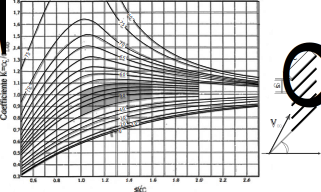
\includegraphics[width=.95\linewidth]{fig/EffSchiera.pdf}
  \captionof{figure}{}
  \label{fig:EffSchiera}
\end{minipage}
\end{figure}
C'è poi la possibilità di correlare per un profilo isolato le relazioni tra angolo di attacco e coefficienti di lift e di drag (Figura \ref{fig:cdcl}). Per quanto riguarda il coefficiente di lift si avrà una parte sostanzialmente lineare mentre il coefficiente di drag è via via crescente. Si arriva ad un punto di stallo in cui c'è una rapida diminuzione del valore di $c_L$ e un rapido aumento di $c_D$; per questo motivo si preferisce lavorare nella zona lineare di variazione di $c_L$.\\
\'E possibile valutare le prestazioni di una schiera di assegnata solidità cercando una correlazione con quello che succede su un profilo isolato. Statisticamente si diagramma anche cosa succede tra un coefficiente $k$ (definito come il rapporto tra il coefficiente di lift del profilo in schiera e coefficiente di lift di profilo isolato $c_{L \infty}$) e l'inverso della solidità della schiera al variare dell'angolo di calettamento (Figura \ref{fig:EffSchiera}). Il range di solidità al quale si fa riferimento varia tra $1$ e $ 1.5 \div 1.6$, non si va oltre $2$. L'angolo di calettamento della schiera è tra i $45^{\circ} \div 52^{\circ}$ come si vede tracciando le linee orizzontali della zona evidenziata nella figura \ref{fig:EffSchiera}. In questo range il rapporto $c_L / c_{L \infty}$ è molto vicino all'unità e quindi la correlazione è alta.\\
Lavorando all'interno di questi range quindi, in fase di progettazione è possibile usare i dati del profilo isolato e correggere il coefficiente utilizzato nella valutazione della schiera secondo questi diagrammi. In contesto industriale si simula fluidodinamicamente direttamente la schiera.
\subsection{Ugelli e diffusori}
Le definizioni sono note e stranote (ugelli portano ad un aumento di velocità a fronte di una riduzione di pressione e vengono utilizzati soprattutto nelle turbine, diffusori viceversa e vengono utilizzati soprattutto nei compressori). 

\'E possibile rappresentare le trasformazioni che si verificano all'interno di ugelli e diffusori sul piano $h-s$ con una trasformazione non isoentropica.
\begin{figure}
\centering
\begin{minipage}{.5\textwidth}
  \centering
  \includegraphics[width=.6\linewidth]{fig/Ugello.pdf}
  \captionof{figure}{Ugello}
  \label{}
\end{minipage}%
\begin{minipage}{.5\textwidth}
  \centering
  \includegraphics[width=.6\linewidth]{fig/Diffusore.pdf}
  \captionof{figure}{Diffusore}
  \label{}
\end{minipage}
\end{figure}
\\Nel caso di ugelli per $Ma < 0.3$ si può scrivere:
\begin{align*}
\eta_{is} = \cfrac{h_{1} - h_2}{h_1-h_{2s}} =\cfrac{\frac{c_2^2}{2}-\frac{c_1^2}{2}}{\frac{c_{2s}^2}{2}-\frac{c_1^2}{2}} = \cfrac{c_2^2 - c_1^2}{c_{2s}^2 - c_1^2}
\end{align*}
\begin{align*}
\begin{cases}
p_{01} = p_1 + \cfrac{1}{2} \rho c_1^2 \;\;\;\;& \to  \;\;\;\; c_1^2 = \cfrac{2}{\rho} (p_{01} - p_1)\\
p_{01} = p_2 + \cfrac{1}{2} \rho c_{2s}^2 \;\;\;\;& \to  \;\;\;\; c_{2s}^2 = \cfrac{2}{\rho} (p_{01} - p_2)\\
p_{02} = p_2 + \cfrac{1}{2} \rho c_2^2 \;\;\;\;& \to  \;\;\;\; c_2^2 = \cfrac{2}{\rho} (p_{02} - p_2)
\end{cases}
\end{align*}
Sostituendo queste relazioni nell'espressione del rendimento si ottiene:
\begin{align*}
\eta_{is} = \cfrac{p_{02} - p_2 - (p_{01} - p_1)}{\cancel{p_{01}} - p_2 - (\cancel{p_{01}} - p_1)}=\cfrac{p_{02} - p_2 -p_{01} + p_1}{p_1-p_2}=1- \cfrac{\Delta p_0}{p_1 - p_2}
\end{align*}
con $\Delta p_0=p_{01}-p_{02}$ che rappresenta la perdita tra ingresso e uscita.

Per i diffusori si consideri sempre $Ma<0.3$ e si possono usare le stesse espressioni; si ottiene un rendimento isoentropico come segue:
\begin{align*}
\eta_{is} = \cfrac{h_{2s}-h_1}{h_2-h_1} =\cfrac{\frac{c_1^2}{2}-\frac{c_{2s}^2}{2}}{\frac{c_1^2}{2}-\frac{c_2^2}{2}}= \cfrac{c_1^2 - c_{2s}^2}{c_1^2 - c_2^2}
\end{align*}
\begin{align*}
\eta_{is} = \cfrac{\cancel{p_{01}} - p_1 - (\cancel{p_{01}} - p_2)}{p_{01} - p_1-(p_{02} - p_2)} = \cfrac{p_2 - p_1}{p_2 - p_1 + (p_{01} - p_{02})} = \cfrac{1}{1+ \cfrac{\Delta p_0}{p_2 - p_1}}
\end{align*}
L'utilizzo di un rendimento isoentropico è meno espressivo nel caso di un diffusore, in quanto ha maggior significato fisico qual è l'entità di $ \Delta p$ recuperabile rispetto la parte eccedente la pressione statica in ingresso.\\
Definendo il coefficiente di recupero di pressione come:
\begin{align*}
c_p = \cfrac{p_2 - p_1}{p_{01} - p_1}
\end{align*}
si cerca il legame tra coefficiente di recupero di pressione e rendimento isoentropico di un diffusore:
\begin{align*}
\cfrac{1}{\eta_{is}} = \cfrac{p_2 - p_1 + (p_{01} - p_{02})}{p_2 - p_1} = \cfrac{p_{01} - p_1 - (p_{02} - p_2)}{p_2-p_1} = \cfrac{1}{c_P} - \cfrac{p_{02} - p_2}{p_2 - p_1}
\end{align*}
Si può definire un coefficiente di pressione ideale ottenuto ipotizzando di avere un recupero di pressione senza perdite:
\begin{align*}
c_{pi} = \cfrac{p_2 - p_1 + (p_{01} - p_{02})}{p_{01} - p_1}
\end{align*}
Considerando:
\begin{align*}
\begin{cases}
p_{2} = p_{02} - \cfrac{1}{2} \rho c_2^2\\
p_{1} = p_{01} - \cfrac{1}{2} \rho c_1^2
\end{cases}
\end{align*}
e considerando la conservazione della portata in massa ($\rho c A=cost$), si può scrivere $c_{pi}$ in funzione di $A_1$ e $A_2$, aree di ingresso e uscita del diffusore:
\begin{align*}
c_{pi} = \cfrac{c_1^2 - c_2^2}{c_1^2} = 1 - \left( \cfrac{c_2}{c_1}\right)^2 = 1- \left(\cfrac{A_1}{A_2} \right)^2 =1-\cfrac{1}{A_R^2}
\end{align*}
con $A_R$ aspect ratio (rapporto tra sezione di uscita e sezione di ingresso). A questo punto si ottiene un rapporto:
\begin{align*}
\cfrac{c_P}{c_{pi}} = \cfrac{p_2-p_1}{p_{01}-p_1} \cdot \cfrac{p_{01}-p_1}{(p_2-p_1)+(p_{01}-p_{02})}= \eta_{is}
\end{align*}
Il diffusore funziona bene finché l'aspect ratio è molto piccolo altrimenti si verificano le condizioni per lo stallo a meno di non prevedere un diffusore con una geometria molto allungata. Per questo motivo l'angolo $\Theta$ vale pochi gradi soprattutto con diffusori corti, altrimenti ci sarebbe una ricircolazione di flusso sulle pareti e una diminuzione delle prestazioni. 
\begin{figure}
\centering
  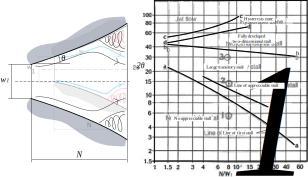
\includegraphics[width=.7\textwidth]{fig/stallo.pdf}
\caption{Zone di stallo}
\label{fig:stallo}
\end{figure}
\begin{figure}
\centering
  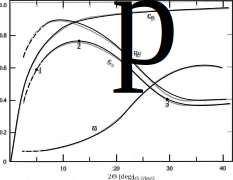
\includegraphics[width=.5\textwidth]{fig/DiffPerf.pdf}
\caption{Tipiche curve di performance per un diffusore bidimensionale con $N/W_1 = 0.8$}
\label{fig:DiffPerf}
\end{figure}
\\In figura \ref{fig:DiffPerf} sono rappresentate le tipiche curve di un diffusore.
\section{Schiere palari}
Le schiere di pale possono essere:
\begin{itemize}
	\item di espansione: si ha un'accelerazione del flusso e quindi un comportamento simile ad un ugello. Vista l'analogia con l'ugello, il rendimento isoentropico di queste schiere è esprimibile come:
	\begin{align*}
	\eta_{is} = 1- \cfrac{\Delta p_0}{p_1 - p_2}
	\end{align*}
	Sapendo però che la perdita di pressione tra ingresso e uscita può essere scritta nei termini della forza assiale sviluppata:
	\begin{align*}
	p_1-p_2 = \cfrac{F_a}{s}
	\end{align*}
	e la forza assiale può essere scritta come:
	\begin{align*}
	F_a=  - F_t \tan \alpha_{\infty} + s \Delta p_0
	\end{align*}
	si può scrivere il rendimento isoentropico come:
	\begin{align*}
	\eta_{is} = \cfrac{1}{1- \cfrac{\Delta p_0 s}{F_t \tan \alpha_{\infty}}}
	\end{align*}
	\item  di compressione: si ha una trasformazione della velocità in pressione e quindi un comportamento simile ad un diffusore. Vista l'analogia con il diffusore, il rendimento isoentropico è espresso come:
	\begin{align*}
	\eta_{is} = \cfrac{1}{1 + \cfrac{\Delta p_0}{p_2-p_1}}
	\end{align*}
	Seguendo un percorso simile a quello della schiera di espansione, si può scrivere:
	\begin{align*}
	\eta_{is} = 1- \cfrac{\Delta p_0 s}{F_t \tan \alpha_{\infty}}
	\end{align*}
	Utilizzando le espressioni viste precedentemente di forza tangenziale, differenza di pressione totale, $V_\infty$ e $V_2$, si risale alla relazione che esprime il secondo termine dell'espressione di $\eta_{is}$:
	\begin{align*}
	\begin{cases}
	F_t = c_F \cfrac{1}{2} \rho c V_{\infty}^2\\
	\Delta p_0 = y \cfrac{1}{2} \rho V_2^2\\
	V_{\infty} = \cfrac{V_a}{\cos \alpha_{\infty}}\\
	V_2 = \cfrac{V_a}{\cos \alpha_2}
	\end{cases}
	\;\;\;\; \rightarrow \;\;\;\;
	\cfrac{\Delta p_0 s}{F_t \tan \alpha_{\infty}} = \cfrac{y}{c_F \tan \alpha_{\infty}} \cdot \cfrac{\cos^2 \alpha_{\infty}}{\sigma \cdot \cos^2 \alpha_2}
	\end{align*}
	\\Andando a considerare poi le relazioni tra i coefficienti di pressione, di forza, di lift e di drag è possibile esprimere il rendimento isoentropico in funzione dei parametri di lift e di drag.
	\begin{align*}
	\begin{cases}
	c_P = \left(  \cfrac{s}{c} \right) y \left( \cfrac{V_2}{V_{\infty}}  \right)^2 - c_F \tan \alpha_{\infty}\\
	c_F = 2 \bigg(\cfrac{s}{c} \bigg) \cos ^ 2 \alpha_{\infty}(\tan \alpha_1 - \tan \alpha_2)\\
	c_L = c_F \cos \alpha_{\infty} - c_P \sin \alpha_{\infty}\\
	c_D = c_F \sin \alpha_{\infty} + c_P \cos \alpha_{\infty}
	\end{cases}
	\;\; \Rightarrow \;\;
	\end{align*}
	\begin{align*}
	\begin{cases}
	c_L = 2 \left(  \cfrac{s}{c} \right) (\tan \alpha_1 - \tan \alpha_2) \cos \alpha_{\infty} - c_D \tan \alpha_{\infty}\\
	c_D= \left(  \cfrac{s}{c} \right) y \cfrac{\cos^3 \alpha_{\infty}}{\cos \alpha_2}
	\end{cases}
	\Rightarrow
	\eta_{is} = 1- \cfrac{2 c_D}{c_L \sin (2 \alpha_{\infty})}
	\end{align*}
	Per rendere elevato il rendimento della schiera bisogna cercare il massimo del rapporto $c_L/c_D$, che rappresenta quindi l'efficienza del profilo. Esiste un tratto significativo di funzionamento in cui il rapporto $c_L/c_D$ rimane costante e questo corrisponde alle condizioni di funzionamento ottimo.\\
	Derivando il rendimento per $\alpha_{\infty}$ si trova il valore dell'angolo che rende massimo il rendimento:
	\begin{align*}
	\cfrac{\partial \eta_{is}}{\partial \alpha_{\infty}} = 0 \;\;\;\;\;\;\;\; \cfrac{c_D}{c_L} = cost.
	\end{align*}
	\begin{align*}
	\eta_{is,max} = 1- \cfrac{2 c_D}{c_L}
	\end{align*}
	Il valore di $\alpha_{\infty}$ ottimale è di $45$ gradi.
\end{itemize}

Si studiano ora i triangoli di velocità della schiera in movimento (Figura \ref{fig:SchiereCompr}); i triangoli invece di essere chiusi sul vettore velocità vengono rappresentati partendo dallo stesso punto di origine. 
\begin{figure}
\centering
  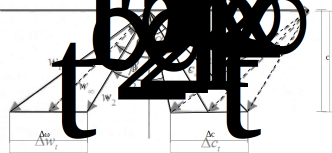
\includegraphics[width=\textwidth]{fig/SchiereCompr.pdf}
\caption{Schiere in movimento (compressore)}
\label{fig:SchiereCompr}
\end{figure}
\\Si può quindi calcolare la forza tangenziale data dalla variazione delle velocità relative tra ingresso e uscita:
\begin{align*}
\Delta c_t = c_{2t} - c_{1t} = \omega_{1t} - \omega_{2t} = |\Delta \omega_t |
\end{align*}
\begin{align*}
F_t = s \rho c_a (\omega_{1t} - \omega_{2t})
\end{align*}
\\Partendo dalle definizioni di potenza, portata in massa e forza tangenziale si definisce il lavoro unitario:
\begin{align*}
\begin{cases}
P=F_t \cdot u\\
\dot{m} = \rho s c_a\\
F_t = c_F \cfrac{1}{2} \rho c \omega_{\infty}^2 = c_F \cfrac{1}{2} \rho c \cfrac{c_a^2}{\cos^2 \beta_{\infty}}
\end{cases} \;\;\;\;
\Rightarrow \;\;\;\;
L_u = \cfrac{P}{\dot{m}}= \cfrac{F_t \cdot u}{\rho s c_a}
\end{align*}
\begin{align*}
L_u = \cfrac{c_F \cdot \sigma}{2 \cos^2 \beta_{\infty}} \cdot c_a \cdot u
\end{align*}
\\Con questa espressione si può ora adimensionalizzare il lavoro:
\begin{align*}
\begin{cases}
\psi = \cfrac{L_u}{\omega ^2 D^2} = \cfrac{L_u}{4 u^2}\\
\varphi = \cfrac{Q}{\omega D^3} \propto \cfrac{c_a}{u}
\end{cases} \;\;\;\;
\Rightarrow \;\;\;\;
\psi = \cfrac{c_F \sigma}{8 \cos^2 \beta_{\infty}} \cdot \cfrac{c_a}{u} = \cfrac{c_F \sigma}{8 \cos^2 \beta_{\infty}} \cdot \varphi
\end{align*}
L'ultima espressione rappresenta la curva di funzionamento della macchina in quanto ovviamente il lavoro viene fatto esclusivamente dalle parti rotoriche.

Si può quindi scrivere il rendimento isoentropico sia nel caso di compressione che di espansione:
\begin{multicols}{2}
Compressione
\begin{align*}
\eta_{is} = \cfrac{L_u - \cfrac{\Delta p_0}{\rho}}{L_u} = 1- \cfrac{\cfrac{\Delta p_0}{\rho}}{L_u}
\end{align*}
\break
Espansione
\begin{align*}
\eta_{is} = \cfrac{L_u}{L_u + \cfrac{\Delta p_0}{\rho}} = \cfrac{1}{1+\cfrac{\cfrac{\Delta p_0}{\rho}}{L_u}}
\end{align*}
\end{multicols}
e utilizzando le relazioni note:
\begin{align*}
\begin{cases}
\Delta p_0 = y \cfrac{1}{2} \rho \omega_2^2\\
L_u = \cfrac{c_F \sigma}{2 \cos^2 \beta_{\infty}} \cdot c_a \cdot u\\
\omega_2 = \cfrac{c_a}{\cos \beta_2}\\
\varphi = \cfrac{c_a}{u}
\end{cases}
\end{align*}
si ottengono le espressioni:
\begin{multicols}{2}
Compressione
\begin{align*}
\eta_{is} = 1- \cfrac{y}{c_F} \cdot  \cfrac{cos^2 \beta_{\infty}}{\sigma \cos^2 \beta_2} \cdot \varphi
\end{align*}
\break
Espansione
\begin{align*}
\eta_{is} = \cfrac{1}{1+\cfrac{y}{c_F} \cdot \cfrac{\cos^2 \beta_{\infty}}{\sigma \cos^2 \beta_2} \cdot \varphi}
\end{align*}
\end{multicols}
Unendo la parte statorica e parte rotorica, la variazione di pressione che porta al calcolo del rendimento di uno stadio assumerà l'espressione:
\begin{align*}
\Delta p_0 = \Delta p_{0,stat} + \Delta p_{0,rot}
\end{align*}
\section{Equilibrio radiale}
Con i capitoli precedenti è stato trattato cosa succede nell'attraversamento della schiera in termini macroscopici; per effettuare queste considerazioni bisogna partire dal presupposto che non vi sia un deflusso significativo in direzione radiale assicurandosi quindi che non vi sia trasmissione di forze tra sezioni circolari della macchina.
\begin{figure}[h!]
	\centering
	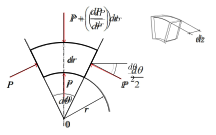
\includegraphics[width=.6\textwidth]{fig/concio.pdf}
	\caption{Equilibrio radiale}
	\label{fig:concio}
\end{figure}
\\Si consideri l'elementino di fluido $dz - d\theta$, figura \ref{fig:concio}, su cui agiscono le forze di pressione. Si calcoli l'equilibrio delle forze:
\begin{align*}
\left( P + \cfrac{dP}{dr} dr \right) (r + dr) d \theta dz - Pr d \theta dz -2P dr dz \sin \frac{d \theta}{2} = r \frac{dP}{dr} dr d \theta dz
\end{align*}
Linearizzando e trascurando i termini del secondo ordine si ottiene un termine che verrà equilibrato dalle forze centrifughe agenti sull'elemento. Affinché il moto non abbia componenti radiali deve quindi accadere:
\begin{equation}
\rho r d \theta dr dz \cdot \frac{V_t^2}{r} = r \frac{dP}{dr} dr d \theta dz \;\;\;\; \Rightarrow \;\;\;\; \cfrac{1}{\rho} \cfrac{dP}{dr} = \frac{V_t^2}{r}
\label{eq:EquilibrioRad}
\end{equation}
\subsection{Termodinamica}
Da un punto di vista termodinamico, si scrive l'entalpia di ristagno (ipotizzando un moto valutato su una superficie cilindrica per cui $V_r = 0$):
\begin{align*}
h_0 = h + \cfrac{V^2}{2} = h + \cfrac{1}{2}(V_t^2 + V_a^2)
\end{align*}
Differenziando lungo il raggio si ottiene:
\begin{equation}
\frac{dh_0}{dr} = \frac{dh}{dr} + V_t \frac{V_t}{dr} + V_a \frac{dV_a}{dr}
\label{eq:EntalpiaDiff}
\end{equation}
Considerando ora il primo principio della termodinamica nella seguente forma:
\begin{equation}
Tds = dh - \cfrac{1}{\rho} dP
\label{eq:PrimoPrinc}
\end{equation}
e unendo le equazioni \ref{eq:EntalpiaDiff} e \ref{eq:PrimoPrinc} risulta:
\begin{align*}
\frac{dh_0}{dr} = T \frac{ds}{dr} + \frac{1}{\rho} \frac{dP}{dr} + V_t \frac{dV_t}{dr} + V_a \frac{dV_a}{dr}
\end{align*}
Considerando poi l'equazione \ref{eq:EquilibrioRad} si ottiene:
\begin{align*}
\frac{dh_0}{dr} = T \frac{ds}{dr} + \frac{V_t^2}{r} + V_t \frac{dV_t}{dr} + V_a \frac{dV_a}{dr}
\end{align*}
In questa espressione non c'è più una pressione ma solo i valori di velocità, entalpia ed entropia al variare del raggio. A questo punto è possibile scrivere l'equazione complessiva che rappresenta il legame da imporre per avere un flusso bidimensionale:
\begin{equation}
\boxed{ \frac{dh_0}{dr} - T\frac{ds}{dr} = V_a \frac{dV_a}{dr} + \frac{V_t}{r} \frac{d}{dr}(V_t \cdot r)}
\end{equation}
Questa equazione consente di affrontare due problematiche tipiche della progettazione delle macchine:
\begin{enumerate}
\item Problema diretto (o problema di verifica): nota la geometria di una macchina e la distribuzione radiale dell'angolo $\alpha_{\infty}$, determinare la distribuzione radiale di tutte le grandezza del flusso e termodinamiche.
\item Problema inverso (o problema di progetto): assegnata una certa distribuzione di una grandezza termodinamica o fluidodinamica, trovare qual è la geometria della schiera che la realizza.
\end{enumerate}
\subsection{Ipotesi semplificative}
Si può fare un'ulteriore osservazione semplificativa per la fase di progettazione preliminare. Si impone:
\begin{align*}
\begin{cases}
\cfrac{dh_0}{dr} = 0\\
\cfrac{ds}{dr} = 0 
\end{cases}
\end{align*}
ossia che $h_0$ e la dissipazione siano costanti lungo il raggio. Queste due osservazioni sono abbastanza realistiche. In questo modo si ottiene la relazione semplificata:
\begin{equation}
\boxed{ V_a \frac{d V_a}{dr} + \frac{V_t}{r} \frac{d}{dr}(V_t \cdot r) = 0}
\label{eq:EquilibrioRadSemp}
\end{equation}
\section{Condizione di vortice libero}
Si possono fare ora delle ulteriori osservazioni sulle velocità assiali.\\
\'E possibile ad esempio costruire la macchina imponendo le condizioni di vortice libero:
\begin{equation}
\boxed{V_t \cdot r = cost}
\end{equation}
Unendo l'equazione di vortice libero all'equazione \ref{eq:EquilibrioRadSemp}, si ottiene:
\begin{align*}
V_a=cost
\end{align*}
ossia una velocità assiale costante lungo il raggio.\\
Dal punto di vista dell'entalpia, considerando il rapporto tra una sezione generica e una sezione $i$, sapendo che $h_0 = cost$, si scrive
\begin{align*}
h + \frac{V^2}{2} = h_i + \frac{V_i^2}{2} \;\;\;\; \Rightarrow \;\;\;\; h = h_i	+ \frac{V_i^2 - V^2}{2}
\end{align*}
e quindi, considerando che $V^2=V_t^2+V_a^2$:
\begin{equation}
\frac{h}{h_i} = 1 + \frac{1}{2h_i} (V_{ti}^2+ \cancel{V_a^2}-V_t^2 -\cancel{V_a^2}) = 1 + \frac{V_{ti}^2}{2h_i} \left( 1- \frac{V_t^2}{V_{ti}^2} \right)
\label{eq:RappEnt}
\end{equation}
Ricordando l'equazione di vortice libero:
\begin{align*}
V_t \cdot r = V_{ti} \cdot r_i \;\;\;\; \Rightarrow \;\;\;\; \frac{V_t}{V_{ti}} = \frac{r_i}{r}
\end{align*}
si può scrivere l'equazione \ref{eq:RappEnt} come:
\begin{equation}\label{eq:h_hi}
\boxed{\frac{h}{h_i} = 1 + \frac{V_{ti}^2}{2h_i} \bigg(1 -  \left( \frac{r_i}{r}\right)^2 \bigg)}
\end{equation}
Se si considera un gas perfetto:
\begin{equation}\label{eq:condgasperf}
\begin{cases}
h = \cfrac{a ^ 2}{\gamma - 1} \\
M_{ti} = \cfrac{V_{ti}}{a_i}
\end{cases}
\end{equation}
Queste relazioni permettono di riscrivere l'equazione \ref{eq:h_hi} come:
\begin{equation}
\boxed{\frac{h}{h_i} = 1 + \frac{\gamma -1}{2} M_{ti}^2 \bigg(1 -  \left( \frac{r_i}{r}\right)^2 \bigg) }
\end{equation}
Si possono ora diagrammare, nelle condizioni di vortice libero, tutte le espressioni utili a livello termodinamico. In Figura \ref{fig:VorticeLibero} è rappresentata la variazione del rapporto delle pressioni in funzione del rapporto dei raggi al variare del numero di Mach; questo diagramma è significativo vista la relazione tra rapporto delle entalpie e delle pressioni:
\begin{align*}
	\cfrac{p}{p_i} = \left( \cfrac{h}{h_i} \right)^{\frac{\gamma}{\gamma - 1}}
\end{align*}
\'E possibile notare come c'è sempre un valore minimo di raggio oltre il quale non ci si può spingere.
\begin{figure}
\centering
  \includegraphics[width=.75\textwidth]{fig/VorticeLibero.pdf}
\caption{Rapporto delle pressioni in funzione del rapporto dei raggi al variare del numero di Mach per un flusso a vortice libero}
\label{fig:VorticeLibero}
\end{figure}
\section{Vortice forzato}
Questo tipo di condizione non si realizza nella realtà nelle fasi di progettazione della macchina o nel suo funzionamento. Tuttavia viene utilizzata per mitigare le problematiche relative al vortice libero introducendo una distribuzione di velocità diversa da quella prevista dal vortice libero.\\
Condizione di vortice forzato:
\begin{equation}
\boxed{\frac{V_t}{r} = cost}
\label{eq:VortForz}
\end{equation}
Questo significa che il deflusso della macchina si comporta effettivamente come un moto rigido.\\
Si ricordano le equazioni di partenza, ovvero quella di equilibrio radiale e le ipotesi semplificative:
\begin{equation}
\begin{cases}
\cfrac{dh_0}{dr} - T\cfrac{ds}{dr} = V_a \cfrac{dV_a}{dr} + \cfrac{V_t}{r} \cfrac{d}{dr}(V_t \cdot r)\\
\cfrac{dh_0}{dr} - T\cfrac{ds}{dr} = 0
\end{cases}
\label{eq:vorticeForzato}
\end{equation}
Allora considerando la generica sezione $i$:
\begin{align*}
\frac{V_t}{r} = \frac{V_{ti}}{r_i} \;\;\;\; \Rightarrow \;\;\;\; V_t = V_{ti} \frac{r}{r_i}
\end{align*}
Introducendo questa relazione e sostituendola a $V_{t}$ in \ref{eq:vorticeForzato}, si ottiene:
\begin{align*}
\frac{d}{dr}\bigg( \frac{V_a^2}{2} \bigg) + \frac{V_{ti}}{r_i} \frac{d}{dr} \bigg(\frac{V_{ti}}{r_i} r^2 \bigg) = 0
\end{align*}
Si tratta di un'equazione differenziale del primo ordine, risolvibile analiticamente:
\begin{equation}
\frac{d}{dr} \bigg( \frac{V_a^2}{2} \bigg) = -2 \bigg( \frac{V_{ti}}{r_i} \bigg) ^2 \cdot r
\;\;\;\; \Rightarrow \;\;\;\; 
\bigg( \frac{V_a^2}{2} \bigg) = - V_{ti}^2 \bigg(\frac{r}{r_i} \bigg)^2 +C
\label{eq:SolCost}
\end{equation}
Bisogna determinare la costante $C$. Nella sezione i-esima la velocità assiale e raggio avranno rispettivamente valori $V_{ai}$ e $r_i$, quindi:
\begin{align*}
\begin{cases}
V_a=V_{ai}\\
r=r_i
\end{cases}
\;\;\;\; \Rightarrow \;\;\;\;
C = \frac{V_{ai}^2}{2} +  V_{ti}^2
\end{align*}
Sapendo che:
\begin{align*}
\frac{V_{ti}}{V_{ai}} = \tan \alpha_i
\end{align*}
si può scrivere la \ref{eq:SolCost} nella forma completa:
\begin{equation}
\boxed{ \bigg( \frac{V_a}{V_{ai}} \bigg)^2 = 1- 2 \tan^2 \alpha_i \bigg[ \bigg( \frac{r}{r_i} \bigg)^2 -1 \bigg] }
\label{eq:RappVol}
\end{equation}

Si prosegue e si determina anche l'andamento dell'entalpia in funzione del raggio. Si ricorda l'espressione per l'entalpia totale:
\begin{align*}
h = h_i + \frac{V_i^2 - V^2}{2}
\end{align*}
A questo punto si calcola il rapporto tra l'entalpia di riferimento e l'entalpia in una generica sezione $i$:
\begin{align*}
\frac{h}{h_i} = 1+ \frac{1}{2 h_i} (V_{ti}^2 + V_{ai}^2- V_t^2 -V_a^2)
\end{align*}
Raccogliendo i termini $V_{ti}$ e $V_{ai}$ si ottiene:
\begin{align*}
\frac{h}{h_i} = 1+ \frac{V_{ti}^2}{2 h_i} \bigg[ 1- \bigg( \frac{V_t}{V_{ti}} \bigg)^2 \bigg] + \frac{V_{ai}^2}{2 h_i} \bigg[ 1- \bigg( \frac{V_a}{V_{ai}} \bigg)^2 \bigg]
\end{align*}
Si possono fare delle ulteriori considerazioni ricordando la \ref{eq:RappVol} e le seguenti espressioni:
\begin{align*}
\begin{cases}
\cfrac{V_t}{V_{ti}} = \cfrac{r}{r_i}\\
\cfrac{V_{ti}}{V_{ai}} = \tan \alpha_i
\end{cases}
\end{align*}
si perviene a:
\begin{equation}
\boxed{ \frac{h}{h_i} = 1+ \frac{V_{ti}^2}{2h_i} \bigg[ \bigg( \frac{r}{r_i} \bigg)^2 -1 \bigg] }
\label{eq:rappEntalpie}
\end{equation}
Questo significa che a seconda dell'angolo $\alpha_i$, la distribuzione delle velocità assiali non è più uniforme lungo il raggio; si vede chiaramente questo comportamento nel diagramma in Figura \ref{fig:TurboFan}.
\begin{figure}
\centering
  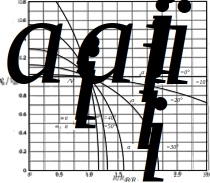
\includegraphics[width=.8\textwidth]{fig/VortForz.pdf}
\caption{Velocità assiale in funzione del raggio per un flusso a vortice forzato}
\label{fig:TurboFan}
\end{figure}
\\Naturalmente si può ricavare l'andamento delle pressioni (Figura \ref{fig:PVortForz}) e delle entalpie ricordando che:
\begin{align*}
\frac{p}{p_i} = \frac{h}{h_i}^{\frac{k}{k-1}}
\end{align*}
\begin{figure}
\centering
  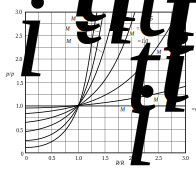
\includegraphics[width=.8\textwidth]{fig/PVortForz.pdf}
\caption{}
\label{fig:PVortForz}
\end{figure}
\\Come nel caso del vortice libero, ricordando le condizioni \ref{eq:condgasperf}, si può scrivere:
\begin{align*}
\boxed{\frac{h}{h_i} = 1 + \frac{k-1}{2} M_{ti}^2 \bigg[ \bigg(\frac{r}{r_i} \bigg)^2-1 \bigg]}
\end{align*}
\\L'entalpia varia con il rapporto dei raggi in maniera quadratica e con una costante che dipende dal numero di Mach tangenziale. Si vede che con raggio pari a $0$ le pressioni non sono nulle (al contrario del caso di vortice libero). Sebbene non si realizzerà mai una macchina con vortice forzato, nel caso il diametro all'albero sia particolarmente ridotto si può utilizzare una distribuzione diversa dal vortice libero. 
\subsection{A valle del vortice forzato}
Cosa succede però a valle della palettatura dopo aver attraversato un vortice forzato? Si impone la condizione di entalpia totale costante al variare del raggio:
\begin{align*}
\frac{dh_{0}}{dr} = 0
\end{align*}
e si vuole valutare se si conserva nella sezione successiva.
\begin{center}
\begin{tabular}{l l l l l l l l l l l l l l l}
	Sezione 1 & & & & & & & & & & & & & & Sezione 2\\
	$
	\begin{cases}
		h_{01} = cost\\
		V_{t1} = K_1 \cdot r
	\end{cases}$ & & & & & & & & & & & & & & $V_{t2} = K_2 \cdot r$
\end{tabular}
\end{center}
Si può calcolare il lavoro scambiato come differenza di entalpia totale:
\begin{align*}
\begin{split}
L_u=h_{02} - h_{01} &= u (V_{t2} - V_{t1} ) = \omega r (K_2 r - K_1 r) \\
&= \omega (K_2 - K_1) r^2 = \Delta h_{012}
\end{split}
\end{align*}
ovvero $\Delta h \propto r^2 \; \Rightarrow \; h_{02} \neq  cost$. Quindi attraversando la macchina, a seconda del raggio a cui ci si trova, cambia il lavoro scambiato dalla macchina; questa condizione è pressoché impossibile da mantenere in fase di progettazione e per questo non si utilizza il vortice forzato in questa fase del progetto.\\
Si vede ora cosa succede calcolando il differenziale dell'entalpia rispetto al raggio:
\begin{align*}
\begin{split}
\cfrac{d \Delta h_{012}}{dr} &= \cfrac{d ( h_{02}-h_{01})}{dr} = \cfrac{dh_{02}}{dr} = V_a \cfrac{dV_a}{dr} + \cfrac{V_t}{r} \cfrac{d}{dr} (V_t \cdot r) = \\
& =2 \omega (K_2 - K_1) r = \cfrac{d}{dr} \bigg( \cfrac{V_{a2}^2}{2} \bigg) + K_2 \cfrac{d}{dr} (K_2 r^2)
\end{split}
\end{align*}
Questa è un'equazione differenziale lineare di primo ordine che rappresenta l'equilibrio radiale, e si può risolvere integrando e ottenendo:
\begin{equation}
\boxed{V_{a2}^2 = -2 \left[ K_2^2 - \omega \left( K_2 - K_1 \right) \right] r^2 + C}
\label{eq:valleVorticeForzato}
\end{equation}
La costante C si ottiene integrando su tutta la sezione la portata in massa:
\begin{align*}
\frac{\dot{m}}{2 \pi \rho} = \int_{rh}^{rs} V_{a1} r dr = \int_{rh}^{rs} V_{a2} r dr
\end{align*}
L'uguaglianza degli integrali rappresenta che la portata entrante nella sezione 1 deve essere uguale alla portata che entra nella sezione 2 (integrale da raggio dell'hub a raggio dello shroud in Figura \ref{fig:hubshroud}).
\begin{figure}[h]
\centering
  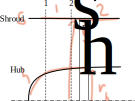
\includegraphics[width=.4\textwidth]{fig/HubShroud.pdf}
\caption{}
\label{fig:hubshroud}
\end{figure}
\section{Vortice generico}
Spesso nella progettazione delle macchine assiali si usa una soluzione mista tra vortice libero e forzato. Si parla di vortice generico:
\begin{align*}
\begin{cases}
V_{t1} = a \cdot r^n - \frac{b}{r}\\
V_{t2} = a \cdot r^n + \frac{b}{r}
\end{cases}
\end{align*}
Definizioni (blending = miscelazione):
\begin{itemize}
\item $n=0$: zero power blending
\item $n=1$: fast power blending
\end{itemize}
Il lavoro effettuato vale quindi:
\begin{align*}
L_u = h_{02} - h_{01} = u \left( V_{t2} - V_{t1} \right) = 2 \cdot b \cdot \omega
\end{align*}
\'E da notare che il lavoro effettuato non varia con il raggio.\\
Per $n=1$ si ha una palettatura a grado di reazione costante; infatti, considerando $V_{a2} \simeq V_{a1}$ (non è del tutto vero ma si assume la differenza piccola), si può scrivere:
\begin{align*}
\begin{split}
	R &= 1 - \frac{V_2^2 - V_1^2}{2 L_u} = 1 - \frac{V_{t2}^2 + \cancel{V_{a2}^2} - V_{t1}^2 - \cancel{V_{a1}^2}}{2 L_u}=\\
	 &= 1 - \frac{\cancel{\left( V_{t2} - V_{t1} \right)} \left( V_{t2}+ V_{t1} \right)}{2 u \cancel{\left( V_{t2}- V_{t1} \right)}} = 1- \frac{\left( V_{t2}+ V_{t1} \right)}{2 u} = 1-\frac{a}{\omega} = cost
\end{split}
\end{align*}
\subsection{Angolo di palettatura costante}
Si immagini ora di voler costruire una macchina con angolo di palettatura costante, ossia con il bordo di attacco rettilineo e solo la coda della palettatura cambia l'angolo.
\begin{align*}
\frac{V_t}{V_a} = \tan \alpha = cost
\end{align*}
Ci si chiede dunque come variano $V_t$ e $V_a$ al variare di $r$ rispettando l'equilibrio radiale.
Si avrà:
\begin{align*}
\frac{V}{V_i} = \frac{V_a}{V_{ai}} = \frac{V_t}{V_{ti}} = \bigg(\frac{r_i}{r} \bigg)^{\sin^2 \alpha}
\end{align*}
Con le solite ipotesi semplificative:
\begin{align*}
\begin{cases}
\cfrac{dh_0}{dr} = 0\\
\cfrac{ds}{dr} = 0 
\end{cases} \;\;\;\; \text{e} \;\;\;\;\;\;
\frac{d}{dr} \bigg(\frac{V_a^2}{2} \bigg) + \frac{V_t}{r} \frac{d}{dr}(V_t \cdot r) = 0
\end{align*}
sapendo inoltre che:
\begin{align*}
\begin{cases}
V_a = V \cos \alpha\\
V_t = V \sin \alpha
\end{cases}
\end{align*}
e facendo le opportune sostituzioni, si perviene a:
\begin{align*}
\frac{dV}{dr} + \frac{V}{r} \sin^2 \alpha = 0
\end{align*}
L'equazione differenziale è leggermente più complessa; la soluzione generica è di tipo esponenziale e bisogna sempre andare a determinare la costante generica.
\begin{align*}
y' + \varphi(x)y + \psi(x) = 0 
\end{align*}
\begin{align*}
y = e^{-\int \varphi(x)dx} \bigg[ C- \int \psi(x) e^{\int \varphi(x)dx} dx \bigg] 
\end{align*}
Nel caso in analisi $\psi(x) = 0$ quindi:
\begin{align*}
V = e^{-\int \frac{\sin^2 \alpha}{r}dr}\cdot C = r^{-\sin^2 \alpha} \cdot C
\end{align*}
Per $r=r_i$ e $V=V_i$ allora:
\begin{align*}
C = \frac{V_i}{r_i^{-\sin^2 \alpha}}
\end{align*}
Questo porta ad un'espressione del rapporto tra le entalpie pari a:
\begin{align*}
\boxed{ \frac{h}{h_i} =  1+ \frac{V_{ti}^2}{2 h_i \sin^2 \alpha} \bigg[1- \bigg(\frac{r_i}{r} \bigg) ^{2 \sin^2 \alpha} \bigg]}
\end{align*}
Si tratta di una soluzione adottata per le macchine a vapore che possiedono delle palettature molto massicce, con sviluppo radiale limitato che permettono di ottenere un andamento delle velocità assiali come in Figura \ref{fig:AngPalCost}. Questa è una distribuzione che non ha limiti teorici, si può sempre fare una macchina a bordo d'ingresso rettilineo; essa rappresenta un caso intermedio tra un vortice libero e un vortice forzato.\\
\'E possibile osservare nelle figura \ref{fig:TurboFan1} come cambia la svergolamento della palettatura tra hub e shroud di una turbina e di un compressore nel caso di corrente a vortice libero; questa forma particolare ha il fine di mantenere le condizioni di equilibrio radiale visto che cambia il profilo di velocità della corrente.
\begin{figure}
\centering
  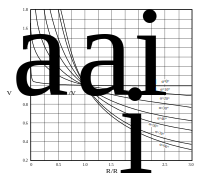
\includegraphics[width=.8\textwidth]{fig/AngPalCost.pdf}
\caption{}
\label{fig:AngPalCost}
\end{figure}
\begin{figure}
\centering
  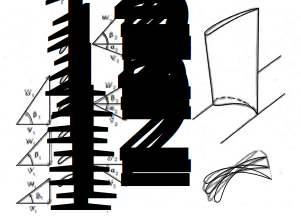
\includegraphics[width=.8\textwidth]{fig/TurboFan.pdf}
\caption{Profili e triangoli delle velocità per un rotore di turbo fan a vortice libero ($r_{Tip}/r_{Hub} =2$)}
\label{fig:TurboFan1}
\end{figure}
\begin{figure}
\centering
  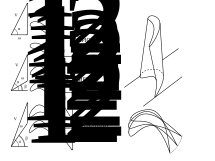
\includegraphics[width=.8\textwidth]{fig/TurbVortLib.pdf}
\caption{Profili e triangoli delle velocità per un rotore di uno stadio di bassa pressione di turbina a vapore o a gas ($r_{Tip}/r_{Hub} =1.4$)}
\label{fig:TurbVortLib}
\end{figure}
\section{Portata in un condotto anulare}
Si analizza ora quali sono le altre particolarità del flusso nell'attraversamento della macchina, in particolare quello che accade in un condotto anulare. Si definisce la portata generica tra l'hub e lo shroud integrando tra questi due estremi:
\begin{align*}
\dot{m} = 2 \pi \int_{rh}^{rs} \rho V_a r dr
\end{align*}
con $V_a$ dipendente dal vortice utilizzato per progettare l'andamento dei triangoli di velocità ai diversi raggi. Questa espressione è limitata al caso di flusso comprimibile.\\
Considerando una sezione anulare piccola, quindi $V_a = cost$, si scrive:
\begin{align*}
\dot{m} = S \rho V_a = S \frac{\rho V_a}{\rho_0 a_o}\rho_0 a_0 = S \rho_0 a_0 \Phi = cost \cdot \Phi
\end{align*}
\begin{equation}\label{eq:portanulare}
\Phi = \frac{\rho}{\rho_0} \frac{V_a}{a_0}
\end{equation}
La definizione \ref{eq:portanulare} rappresenta la portata adimensionalizzata rispetto le condizioni di ristagno a monte sotto l'ipotesi di gas perfetto $p = \rho RT$ e flusso isoentropico $p \rho^{-k} = cost$; si analizzano i rapporti che compaiono in questa definizione.\\
Combinando le ipotesi di gas perfetto e flusso isoentropico si può scrivere:
\begin{align*}
\frac{\rho}{\rho_0} = \bigg( \frac{T}{T_0} \bigg)^{\frac{1}{k-1}} 
\end{align*}
ma scrivendo:
\begin{align*}
\begin{cases}
a = \sqrt{kRT}\\
a_0 = \sqrt{kRT_0}
\end{cases}
\;\;\;\; \rightarrow \;\;\;\; \frac{\rho}{\rho_0} = \bigg( \frac{a}{a_0} \bigg)^{\frac{2}{k-1}}
\end{align*}
Si sviluppa ora il secondo rapporto:
\begin{align*}
V^2 = 2 (h_0 - h) = 2 c_p (T_0 - T) = 2 \frac{c_p}{kR} (a_0^2 - a^2)
\end{align*}
\begin{align*}
\frac{V^2}{a_0^2} = \frac{2}{k-1} \bigg[ 1- \bigg( \frac{a}{a_0} \bigg)^2 \bigg] = \frac{V_a^2 + V_t^2}{a_0^2}
\end{align*}
\begin{align*}
\frac{V_a}{a_0} = \sqrt{\frac{2}{k-1} \bigg[ 1- \bigg( \frac{a}{a_0} \bigg)^2 \bigg] - \bigg( \frac{V_t}{a_0} \bigg)^2}
\end{align*}
Sostituendo nell'espressione della portata risulta:
\begin{align*}
\Phi = \frac{\rho}{\rho_0} \frac{V_a}{a_0} = f \bigg( \frac{a}{a_0} \bigg)
\end{align*}
Si cerca ora il rapporto critico tra le velocità soniche che massimizzano la portata adimensionalizzata. Se la componente di velocità tangenziale fosse nulla e quindi moto monodimensionale, l'espressione sarebbe quella della velocità critica di un condotto convergente in cui si arriva alla condizione di choking.
\begin{align*}
\frac{d\Phi}{d \bigg( \cfrac{a}{a_0} \bigg)}=0 \;\;\;\; \Rightarrow \;\;\;\; \boxed{ \frac{a^*}{a_0} = \sqrt{\frac{2}{k+1} - \frac{k-1}{k+1} \bigg( \frac{V_t}{a_0} \bigg)^2} }
\end{align*}
con
\begin{align*}
Ma^* = \bigg( \frac{V_a}{a} \bigg)^* = 1
\end{align*}
Diagrammando $\Phi$ in funzione della pressione e delle diverse componenti tangenziali risulta un andamento elicoidale (figura \ref{fd:PortCondAn}).\\
Il flusso in un condotto anulare, può essere supersonico ma non in condizioni di choking, a patto che la velocità assiale sia inferiore a quella acustica. Il choking si ha in tre casi:
\begin{itemize}
\item raggiungimento di velocità sonica $V$ nello statore;
\item raggiungimento di velocità sonica $W$ nel rotore;
\item raggiungimento di velocità sonica assiale nel condotto anulare.
\end{itemize}
\begin{figure}
\centering
  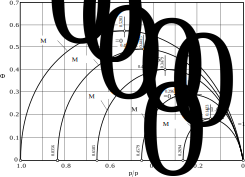
\includegraphics[width=.7\textwidth]{fig/PortCondAn.pdf}
\caption{}
\label{fd:PortCondAn}
\end{figure}
\section{Condizioni di ingolfamento (choking)}
Diminuendo la pressione a valle si aumenta la componente assiale della velocità $V_a$ pur mantenendo $V_t$ se il moto è libero, mentre non è sempre possibile in un moto guidato dalla palettatura. Il segnale di pressione deve riuscire a propagarsi a monte e questo accade solamente se le velocità sono subsoniche.\\
Si considera un punto $P$ da cui si propaga un'onda di pressione all'interno del cono di Mach come mostrato in figura \ref{fd:bloccson1}.
\begin{itemize}
	\item Nel caso di velocità $V_a$ subsonica (figura \ref{fd:bloccson2} sinistra), la perturbazione di pressione si propaga a monte del fronte; in questo modo ad una diminuzione di pressione a valle corrisponde un aumento di velocità a monte.
	\item Nel caso ci si trovi in condizioni limite con $M_a=1$ (figura \ref{fd:bloccson2} a destra), la propagazione del segnale di pressione raggiunge esattamente il punto ``di partenza $P$" della particella; in questo caso non è quindi possibile trasmettere un segnale di pressione a monte e da questo punto in poi il flusso è ingolfato.
	\item Nel caso di velocità $V_a$ supersonica (figura \ref{fd:bloccson1} a destra), la perturbazione di pressione non si propaga a monte del fronte.
\end{itemize} 
\begin{figure}[h!]
\centering
  \includegraphics[width=.8\textwidth]{fig/bloccson1.pdf}
\caption{}
\label{fd:bloccson1}
\end{figure}
\begin{figure}[h!]
\centering
  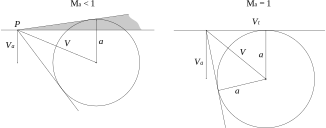
\includegraphics[width=.8\textwidth]{fig/bloccson2.pdf}
\caption{}
\label{fd:bloccson2}
\end{figure}
\section{Componente radiale non trascurabile}
Nel caso ci sia nel flusso una componente radiale non trascurabile, come per esempio nel caso mostrato in figura \ref{fd:comp_rad} in prossimità del mozzo, le equazioni dell'equilibrio radiale imposte sull'elementino di fluido evidenziato si modificano con l'aggiunta di un termine:
\begin{figure}
	\centering
	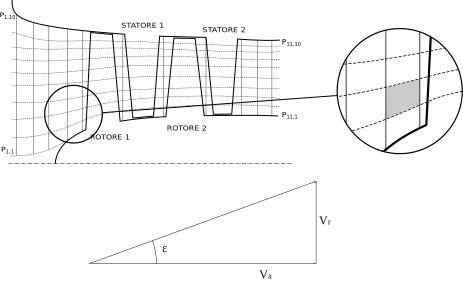
\includegraphics[width=.8\textwidth]{fig/comp_rad.pdf}
	\caption{}
	\label{fd:comp_rad}
\end{figure}
\begin{align*}
\frac{d h_0}{dr} - T\frac{ds}{dr} = V_a \frac{dV_a}{dr} - \boxed{V_a \frac{dV_r}{dz}} + \frac{V_t}{r} \frac{d}{dr} ( V_t \cdot r)
\end{align*}
\section{Moti secondari}
Fino ad ora si è sempre ragionato su un flusso idealizzato che però non corrisponde alla realtà. Nella zona superiore, in cui le pale del rotore sono molto vicine alla cassa, e vicino alla radice delle pale, si forma lo strato limite a parete che innesca i moti secondari a causa appunto dell'interazione del fluido con la parete. Anche se questi moti nascono in zone limitate possono comunque influenzare grosse sezioni.\\
Ci sono quattro diverse tipologie di moti secondari:
\begin{itemize}
\item Vortici di passaggio: sono dovuti ad un moto curvato e una perturbazione dovuta allo strato limite che generano vortici con direzioni opposte. Essi sono dovuti ai diversi gradienti di pressione (figura \ref{fig:VortPass}).
\begin{figure}[h!]
	\centering
	\includegraphics[width=.7\textwidth]{fig/VortPass.pdf}
	\caption{Vortici di passaggio}
	\label{fig:VortPass}
\end{figure}
\item Vortici a ferro di cavallo: sono dovuti all'interazione tra strato limite in ingresso e un ostacolo, come per esempio la palettatura (figura \ref{fd:VortFerrCav}).
\begin{figure}[h!]
	\centering
	\includegraphics[width=.7\textwidth]{fig/VortFerrCav.pdf}
	\caption{Vortici a ferro di cavallo}
	\label{fd:VortFerrCav}
\end{figure}
\item Vortici al bordo di uscita: sono dovuti alla scia di vorticità per lo strato limite al bordo di uscita della schiera (figura \ref{fd:VortVall}).
\begin{figure}[h!]
	\centering
	\includegraphics[width=.6\textwidth]{fig/VortVall.pdf}
	\caption{Vortici al bordo di uscita}
	\label{fd:VortVall}
\end{figure}
\item Vortici di passaggio e di trafilamento: sono dovuti ai giochi tra statore e cassa (figura \ref{fd:VortTraf}).
\begin{figure}[h!]
	\centering
	\includegraphics[width=.8\textwidth]{fig/VortTraf.pdf}
	\caption{Vortici di passaggio e trafilamento}
	\label{fd:VortTraf}
\end{figure}
\end{itemize}




\chapter{Compressori assiali}

\section{Introduzione}
I compressori assiali sono macchine relativamente recenti, si tratta di una macchina nata nel dopoguerra come componente per i gruppi turbina a gas in campo aeronautico. I primi motori aeronautici costituiti da gruppo turbogas sono stati inizialmente costruiti come compressori radiali. C'è una forte correlazione tra compressione ottenibile e rendimento, oggi qualsiasi turbogas salvo eccezioni specifiche si utilizzano compressori assiali. 
\begin{figure}[h!]
\centering
  \includegraphics[width=.8\textwidth]{fig/PrestComp.pdf}
\caption{A destra le curve di rendimento per le macchine assiali. Si nota l'evidente aumento delle prestazioni (in rosso) rispetto alle prime macchine}
\label{fig:PrestComp}
\end{figure}
Nel diagramma in figura \ref{fig:PrestComp} è presente il rendimento del compressore in funzione della velocità specifica (che ricordiamo essere la caratteristica di macchina). Si nota che all'aumentare della velocità specifica si va verso macchine assiali, fino ad un certo punto della storia le macchine assiali non hanno goduto di rendimenti competitivi. In rosso è presentata la curva dello stato attuale dei rendimenti per macchine assiali. 
\begin{figure}
\centering
  \includegraphics[width=.5\textwidth]{fig/hsComp.png}
\caption{1: ingresso statore 2: uscita statore - entrata rotore 3: uscita statore.}
\label{fig:hsComp}
\end{figure}
Nel diagramma termodinamico in figura \ref{fig:hsComp} sono riportati gli stati di rierimento di uno stadio di compressore assiale. Nella parte rotorica avviene il lavoro con un relativo aumento della velocità mentre nello c'è il recupero in termini di pressione. Nello studio della macchina assiale vengono fatte generalmente le seguenti assunzioni:
\begin{itemize}
\item Flusso adiabatico;
\item Stadio ``normale" o ``ripetuto": tutti gli stadi hanno gli stessi profili
\begin{align*}
c_1 = c_2 \Rightarrow h_3-h_1 = h_{03} - h_{01}
\end{align*}
\item Velocità assiale costante (coincide con la velocità meridiana)
\begin{align*}
c_{m1} = c_{m2}
\end{align*}
\item densità costante nello stadio
\begin{align*}
\rho = cost. 
\end{align*}
\end{itemize}
\begin{align*}
\omega_s = \cfrac{\sqrt{\phi}}{\psi^{3/4}} \cdot \sqrt{\bigg( \cfrac{D_e}{D_i} \bigg)^2 -1}
\end{align*}
\begin{align*}
\phi = \frac{Q}{u \cdot S}
\end{align*}
\begin{align*}
\psi = \cfrac{\Delta h_{0is}}{\cfrac{u^2}{2}}
\end{align*}
\section{Lavoro e triangoli di velocità}
Nel rotore si conserva la rotalpia
\begin{equation}
h_1 + \frac{1}{2} w_1^2 = h_2 + \frac{1}{2} w_2^2
\end{equation}
Nello statore si conserva l'entalpia
\begin{equation}
h_2 + \frac{1}{2} c_2^2 = h_3 + \frac{1}{2} c_3^2
\end{equation}
Il lavoro scambiato è quello che avviene nella parte rotorica, definiamo un parametro adimensionale per quest'ultimo
\begin{equation}
\lambda = \frac{u \cdot c_{u2} - u \cdot c_{u1}}{u^2} = \frac{c_{u2} - c_{u1}}{u}
\end{equation}
\begin{figure}
\centering
  \includegraphics[width=.9\textwidth]{fig/triangComp.pdf}
\caption{}
\label{fig:triangComp}
\end{figure}
L'obiettivo è quello di determinare la relazione tra $\lambda$ e cifra di portata $\Phi$. Vado a disegnare i triangoli di velocità relativi allo stadio elementare come mostrato in figura \ref{fig:triangComp}. Ricordo che per definizione la componente meridiana e periferica sono costanti. Posso scrivere le seguenti tre relazioni 
\begin{align*}
c_{u2} = u - w_{u2}
\end{align*}
\begin{align*}
w_{u2} = c_m \tan \beta_2
\end{align*}
\begin{align*}
c_{u1} = c_m \tan \alpha_1
\end{align*}
Posso quindi scrivere
\begin{align*}
\lambda = 1- \frac{w_{u2}}{u} - \frac{c_{u1}}{u} = 1 - \frac{c_m}{u} \left(\tan \beta_2 + \tan \alpha_1 \right)
\end{align*}
Ma definendo  la cifra di portata come
\begin{align*}
\Phi = \frac{c_m}{u}
\end{align*}
Posso finalmente scrivere la cifra di flusso in funzione della cifra di portata, la caratteristica teorica del nostro compressore
\begin{equation}
\lambda = 1 - \Phi \left( \tan \beta_2 + \tan \alpha_1 \right) = 1 - k \cdot \Phi
\end{equation}
Con $k$ costante che dipende dalla geometria della macchina. Si tratta di una rappresentazione molto simile a quella nel caso delle pompe centrifuche nelle quali a seconda del valore di $k$ si ha la curva caratteristica della pompa; questo viene chiarito meglio dal diagramma in figura \ref{fig:CondProg}.
\begin{figure}
\centering
  \includegraphics[width=.4\textwidth]{fig/CondProg.pdf}
\caption{}
\label{fig:CondProg}
\end{figure}
Andiamo ora a definire una condizione particolare di progetto ``lambda design"$\lambda_d$.
\begin{align*}
\lambda_d = 1 - k \cdot \Phi_d, \;\; k = f(\lambda_d,\Phi_d)
\end{align*}
Calcolo ora il rapporto $\lambda/\lambda_d$:
\begin{equation} \label{eq:lambdad}
\frac{\lambda}{\lambda_d} = \frac{1}{\lambda_d} - \frac{\Phi}{\Phi_d} \Bigg( \frac{1-\lambda_d}{\lambda_d} \Bigg), \;\;\; 0.3 < \lambda_d < 0.4
\end{equation}
Si tratta di una famiglia di rette, in figura \ref{fig:LambdaPhiChart} è rappresentato il diagramma caratteristico però in termini di rapporti rispetto alle condizioni di progetto. Si vede che nel caso ideale di $\lambda_d = 1$ il lavoro scambiato sarebbe indipendente dalla portata, sarebbe una situazione abbastanza attraente. 
\begin{figure}
\centering
\begin{minipage}{.5\textwidth}
  \centering
  \includegraphics[width=.9\linewidth]{fig/LambdaPhiChart.pdf}
  \captionof{figure}{}
  \label{fig:LambdaPhiChart}
\end{minipage}%
\begin{minipage}{.5\textwidth}
  \centering
  \includegraphics[width=.9\linewidth]{fig/CarattReal.pdf}
  \captionof{figure}{}
  \label{fig:CarattReal}
\end{minipage}
\end{figure}
Generalmente in un compressore, infatti, la pressione di output è definita mentre la portata è regolata, $\lambda_d = 1$ avrei una macchina perfetta, il rapporto di pressione lo riuscirei sempre a mantenere e basta che regoli la portata per ottenere la pressione voluta. Purtroppo non è così perchè le palettature non si comportano in modo ideale, si hanno separazioni di vela, inspessimenti di strato limite... dal punto di vista realistico si riesce ad ottenere un $\lambda_d$ definito come nell'equazione \ref{eq:lambdad}. 

Come mostrato in figura \ref{fig:CarattReal} otterrò un comportamento non ideale che non avrà andament rettilineo, avrtò quindi un campo di utilizzo essendo limitato sia a portate basse che a portate alte. 

Caratteristica reale:
\begin{equation}
\psi = \frac{\Delta h_{0is}}{u^2} = \lambda \cdot \eta_{is}, \;\;\; \Delta h_{0is} = h_{30is} - h_{10}
\end{equation}

Non abbiamo ancora detto nulla riguardo la forma della pala in funzione del grado di reazione\footnote{Che ricordiamo essere il rapporto tra il salto entalpico elaborato tra parte rotorica e statorica}. 
\begin{align*}
R = \frac{h_2 - h_1}{h_3-h_1} 
\end{align*}
Sapendo che
\begin{align*}
\begin{rcases*}
c_{u2} = u - w_{u2}\\
c_{u1} = u - w_{u1}
\end{rcases*}
\Rightarrow c_{u2} - c_{u1} = w_{u1} - w_{u2} 
\end{align*}
Vado a sviluppare il grado di reazione della macchina applicando la conservazione della rotalpia al numeratore e l'espressione del lavoro euleriano al denominatore:
\begin{align*}
R = \frac{w_1^2 - w_2^2}{2 u (c_{u2} - c_{u1})} &= \frac{(w_{u1} + w_{u2})\cancel{(w_{u1}-w_{u2})}}{2 u \cancel{(c_{u2} - c_{u1})}} =\\
&= \frac{w_{u1} + w_{u2}}{2u} = \\
&= \frac{c_m \left(\tan \beta_1 + \tan \beta_2 \right)}{2 u}
\end{align*}
Definendo poi
\begin{align*}
\tan \beta_{\infty} = \frac{\tan \beta_1 + \tan \beta_2}{2}, \;\; \Phi = \frac{c_m}{u}
\end{align*}
Si ottiene
\begin{equation}
\boxed{R = \Phi \tan \beta_{\infty} = \frac{w_{u \infty}}{u}}
\end{equation}
Lo stesso risultato poteva essere raggiunto nel seguente modo
\begin{equation}
w_{u1} = u - c_{u1} \; \Rightarrow \; R = \frac{1}{2} + \frac{\tan \beta_2 - \tan \alpha_1}{2} \cdot \Phi \simeq \frac{1}{2} + cost \cdot \Phi
\end{equation}
Quello che è importante notare è che:
\begin{align*}
R = 0.5 \to \beta_2 = \alpha_1
\end{align*}
Il grado di reazione è costante con la portata e la palettatura sarà simmetrica.

Per rappresentare lo stadio al variare del grado di reazione andiamo per prima cosa a definire i triangoli di velocità come si vede in figura \ref{fig:StadioRipetuto}.
\begin{figure}
\centering
  \includegraphics[width=\textwidth]{fig/StadioRipetuto.pdf}
\caption{}
\label{fig:StadioRipetuto}
\end{figure}
Sempre facendo riferimento alla figura posso quindi scrivere
\begin{align*}
r \cdot \tan \beta_{\infty} = R 
\end{align*}
\begin{align*}
\lambda = \cfrac{\Delta h_0}{\cfrac{u^2}{2}} = \cfrac{u \Delta c_u}{\cfrac{u^2}{2}} = \cfrac{2 \Delta c_u}{u} = \cfrac{2 \Delta w_u}{u}
\end{align*}
\begin{align*}
\frac{\Delta c_u}{u} = \frac{\Delta w_u}{u} = \frac{\lambda}{2}
\end{align*}
Qual'ora si operi un cambio di portata vediamo che gli unici angoli che si conservano sono $\beta_2$ e $\alpha_1$, la cifra si flusso passa dalle condizioni di design $\Phi_d$ alle condizioni generiche $\Phi$ come si vede in figura \ref{fig:CondFuoriProg}.
\begin{figure}
\centering
  \includegraphics[width=\textwidth]{fig/CondFuoriProg.pdf}
\caption{}
\label{fig:CondFuoriProg}
\end{figure}

Possiamo classificare alcune condizioni notevoli riportate in figura \ref{fig:ComprAssTab}.
\begin{figure}
\centering
  \includegraphics[width=1.2\textwidth]{fig/ComprAssTab.pdf}
\caption{}
\label{fig:ComprAssTab}
\end{figure}
Il primo caso con $r = 1 + \lambda /4$ è particolare in quanto si ha grado di reazione maggiore di uno, lo statore precede infatti il rotore. Mi ritrovo con una velocità di uscita puramente assiale.

Con grado di reazione $r = 1$ le velocità assolute ingresso uscita sono simmetriche.

Con $r = 1 - \lambda/4$ la velocità assoluta è puramente assiale, mentre quella allo scarico non lo è. 

Sono poi rappresentate le geometrie per gradi di reazione sempre più ridotti. 

La soluzione $r = 1/2$ è la più diffusa e utilizzata eccetto per il primo e l'ultimo stadio in cui si vogliono distribuzioni di velocità particolari, velicità assoluta in uscita e poi in ingresso puramente assiale. In questa configurazione si avranno profili uguali ma specchiati, l'intervallo p1 p3 è poi diviso equamente in due parti uguali tra la parte statorica e la parte rotorica. 

\section{Termodinamica}
Vediamo il calcolo del rendimento al variare della portata e del grado di reazione. Partiamo dalla definizione di rendimento isoentropico
\begin{align*}
\eta_{is} = \frac{\Delta h_{is}}{\Delta h_0} = \frac{\Delta p}{\rho \cdot \Delta h_0}
\end{align*}
Dal primo principio:
\begin{align*}
T ds = dh - \frac{dp}{\rho}
\end{align*}
ma
\begin{align*}
ds = 0 \Rightarrow dh = \frac{dp}{\rho}
\end{align*}
Otteniamo quindi
\begin{equation}\label{eq:etadp}
\eta_{is} = \frac{\Delta p}{\rho \cdot \Delta h_0} = \cfrac{\Delta p}{\rho \cdot \cfrac{\lambda}{2} u^2}
\end{equation}
L'incremento di pressione totale si può però ulteriormente sviluppare come somma di incremento di pressione sviluppato nel rotore e nello statore
\begin{align*}
\Delta p = \Delta p_R + \Delta p_S = \frac{F_{aR}}{s_R} + \frac{F_{aS}}{s_S} = \frac{F_{tR} \cdot \tan(\beta_{\infty} - \varepsilon_R)}{s_R} + \frac{F_{tS} \cdot \tan(\alpha_{\infty} - \varepsilon_S)}{s_S}
\end{align*}
Con $\varepsilon_S, \; \varepsilon_R$\footnote{Per quanto riguarda i pedici "s" sta per statore, "r" per rotore.} indice di efficienza del profilo.
Possiamo fare qualche assunzione. I profili hanno drag molto più piccolo del lift quindi
\begin{align*}
\tan \varepsilon_R \simeq \varepsilon_R = \frac{D_R}{L_R} \;\;\;\;\; \tan \varepsilon_S \simeq \varepsilon_S = \frac{D_S}{L_S}
\end{align*}
Utilizzando le componenti di forza del triangolo di velocità si ottiene
\begin{align*}
F_{tR} = \dot{m} \Delta w_u = \overbrace{s_R \cdot \rho \cdot c_m}^\text{$ \dot{m} $} \cdot \overbrace{\lambda \cdot u \cdot \frac{1}{2}}^\text{$\Delta w_u$}  
\end{align*}
Analogamente riesco a fare la stessa cosa per la parte statorica
\begin{align*}
F_{tS} = \dot{m} \Delta c_m = s_S \cdot \rho \cdot \lambda \cdot \Phi \cdot u^2 \cdot \frac{1}{2}
\end{align*}
Andando a sostituire
\begin{align*}
\Delta p = \frac{1}{2} \rho \lambda u^2 \big[ \Phi \tan \left( \beta_{\infty} - \varepsilon_R \right) + \Phi \tan \left( \alpha_{\infty} - \varepsilon_S \right) \big] 
\end{align*}
Ricordando le relazioni
\begin{align*}
R = \Phi \tan \beta_{\infty}
\end{align*}
\begin{align*}
1 - R = \Phi \tan \alpha_{\infty} 
\end{align*}
\begin{align*}
\tan ( \beta_{\infty} - \varepsilon_R ) = \frac{\tan \beta_{\infty} - \tan \varepsilon_R}{1 + \tan \beta_{\infty} \tan \varepsilon_R} \simeq \frac{\tan \beta_{\infty} - \varepsilon_R}{1 + \tan \beta_{\infty} \cdot \varepsilon_R}
\end{align*}
\begin{align*}
\tan (\alpha_{\infty} - \varepsilon_S) \simeq \frac{\tan \alpha_{\infty} - \varepsilon_S}{1 + \tan \alpha_{\infty} \cdot \epsilon_S}
\end{align*}
Ottengo in fine la relazione del salto di pressione in funzione del grado di reazione e di $\lambda$:
\begin{equation}
\Delta p = \frac{1}{2} \rho \lambda u^2 \Bigg[ \frac{R - \varepsilon_R \Phi}{\Phi + \varepsilon_R R} + \frac{1 - R - \varepsilon_S \Phi}{\Phi + \varepsilon_S (1-R)} \Bigg] \cdot \Phi
\end{equation}
Posso dire che epsilon r è circa epsilon s. Il rendimento isoentropico ricordando l'equazione \ref{eq:etadp} diviene:
\begin{equation}
\boxed{ \eta_{is} = \Bigg[ \frac{R - \varepsilon_R \Phi}{\Phi + \varepsilon_R R} + \frac{1 - R - \varepsilon_S \Phi}{\Phi + \varepsilon_S (1-R)} \Bigg] \cdot \Phi }
\end{equation}
Cerco ora il coefficiente di reazione
\begin{align*}
\varepsilon_S \simeq \varepsilon_R = cost = \varepsilon
\end{align*}
\begin{align*}
\frac{d \eta_{is}}{dR} = 0 \Rightarrow R_{opt} = 0.5 per \forall \Phi
\end{align*}
\begin{align*}
\eta_{|R= 0.5} = 2 \Phi \cdot \frac{1- 2 \varepsilon \Phi}{\varepsilon + 2 \Phi}
\end{align*}
Si ha quindi $R_{opt} = 0.5$. 
Naturalmente si vede che il rendimento del compressore è migliorato alla diminuzione di $\varepsilon$.
\begin{align*}
\frac{d\eta_{|R=0.5}}{d \Phi} = 0 \Rightarrow \Phi_{opt} = \frac{1}{2} \left( \sqrt{1 + \varepsilon^2} - \varepsilon \right) \simeq \frac{1 - \varepsilon}{2}
\end{align*}
Determino ora il rendimento ottimale in funzione di $\Phi$
\begin{equation}
\eta_{max} = 1 + 2 \varepsilon^2 - 2 \varepsilon \sqrt{1 + \varepsilon^2} \simeq 1 - 2 \varepsilon \left( 1 - \varepsilon \right)
\end{equation}
\begin{figure}
\centering
  \includegraphics[width=\textwidth]{fig/IsoRendCompAss.pdf}
\caption{Curve isorendimento di uno stadio assiale in funzione del grado di reazione e coefficiente di portata per efficienza del profilo assegnata}
\label{}
\end{figure}

\section{Progettazione della schiera}
\subsection{Correlazioni di Howell}
Sono presenti molteplici correlazioni per progettare una macchina assiale. Noi vedremo un filone di correlazioni, sono datate ma non hanno perso di validità. Anche nella progettazione di una nuova macchina è utile partire da un predimensionamento per poi andare a raffinare con strumenti moderni. Verrà quindi usato come passo preliminare.
Si parte dalle seguenti riflessioni:
\begin{itemize}
\item La deflessione imposta alla corrente è limitata: nell'ordine delle decine di gradi (20, 30 al massimo 40);
\item Profili sottili a bassa curvatura.
\end{itemize}
Le perdite possono quindi essere suddivise in 
\begin{itemize}
\item Perdite di anello;
\item perdite di profilo;
\item perdite per flussi secondari.
\end{itemize}
La perdita di profilo è direttamente correlata al $c_D$, sarà quella in cui si può andare maggiormente a lavorare. 
Il flusso all'interno del compressore è un moto elicoidale. Il flusso lambisce la cassa della macchina, vi sarà quindi un attrito tra fluido e la partete, queste perdite le chiameremo perdite di ``anello".
Le perdite per flussi secondari sono state adeguatamente trattate nel capitolo precedente. 
Si andrà quindi a lavorare sulle perdite di profilo aggiungendo poi le altre due perdite tramite coefficienti di correlazione.

Le perdite di anello inducono un drag aggiuntivo correlato a quanto più è elevato lo sviluppo radiale della pala, definito $H$ lo sviluppo radiale e $s$ passo palare, si può scrivere
\begin{align*}
C_{Da} = 0.02 \cdot \frac{s}{H}
\end{align*}
Abbiamo poi che la perdita per flussi secondari è correlata con il quadrato del coefficiente di portanza, quanto più io ho una portanza elevata quanto più impongo una deviazione, tanto più è probabile che abbia un instaurarsi di moti secondari.
\begin{align*}
C_{Da} = 0.018 \cdot C_L^2
\end{align*}
Posso andare quindi a scrivere un coefficiente di resistenza complessivo
\begin{align*}
C_{Dtot} = C_D + C_{Da} + C_{Ds} = C_D + 0.02 \cdot \frac{s}{H} + 0.018 \cdot C_L^2
\end{align*}
In figura \ref{fig:ComprStageLoss} si vede come le varie perdite inficiano sull'efficienza della schiera.
\begin{figure}
\centering
  \includegraphics[width=\textwidth]{fig/ComprStageLoss.pdf}
\caption{}
\label{fig:ComprStageLoss}
\end{figure}
La progettazione preliminare con la correlazione di Howell, si va a cercare la relazione tra gli angoli geometrici in ingresso e uscita e gli angoli che deve avere il fluido. La prima correlazione di Howell dice che la condizione di riferimento, ovvero la deflessione che la corrente subisce nell'attraversamento delle pale (nominale) $\varepsilon^*$ viene riferita rispetto alla deviazione di stallo $\varepsilon_s$
\begin{equation}
\varepsilon^* = 0.8 \cdot \varepsilon_s
\end{equation}
In figura \ref{fig:Howell} è rappresentato l'andamento della deflessione in funzione dell'angolo di incidenza. Come si nota un tratto pressocchè lineare seguito da un brusco cambiamento di curvatura. Quest'ultimo è facilmente individuabile, risutlta quindi comodo utilizzarlo come punto di riferimento per individuare la deflessione nominale. Cpme deflessione nominale si utilizzarà quindi un valore che va a minimizzare le perdite, tenendo conto poi dei margini di operabilità.  
\begin{figure}
\centering
  \includegraphics[width=\textwidth]{fig/Howell.pdf}
\caption{}
\label{fig:Howell}
\end{figure}
In figura \ref{fig:SchieraDim} si riportano le nomenclature utilizzate in questo capitolo, è rappresentata la differenza tra angoli geometrici e fluidodinamici.
\begin{figure}
\centering
  \includegraphics[width=\textwidth]{fig/SchieraDim.pdf}
\caption{}
\label{fig:SchieraDim}
\end{figure}
La prima correlazione di Howell permette di calcolare gli angoli del flusso attesi da una chiera di data solidità ($\varepsilon = \varepsilon*$).
La seconda correlazione di Howell permette di trovare, noti gli angoli di flusso, i corrispondenti valori degli angoli geometrici della schiera ($\varepsilon = \varepsilon*$).
La terza correlazione di Howell permette di calcolare le prestazioni in off-design, quando $\varepsilon \neq \varepsilon*$ 
In figura \ref{fig:1CorrHowell} è rappresentata la prima correlazione di Howell al variare della solidità della schiera. Si nota che a parità di deflessine nominalre si avrà una maggiore angolo in uscira per schiere più compatte.
\begin{figure}
\centering
  \includegraphics[width=.4\textwidth]{fig/1CorrHowell.pdf}
\caption{}
\label{fig:1CorrHowell}
\end{figure}
Si definisce il campo di validità della relazione
\begin{align*}
\varepsilon^* = f \bigg( \frac{s}{l}, \alpha_2^*, Re \bigg) \;\; 20^{\circ} < \theta < 40^{\circ}
\end{align*}
\begin{align*}
\varepsilon^* = f\bigg(\frac{s}{l}, \alpha_2*\bigg)\;\; Re > 3 \cdot 10^5
\end{align*}
La deflessione nominale è definita come segue
\begin{align*}
\varepsilon^* = \alpha_1^* - \alpha_2^*
\end{align*}
Le curve espresse come relazione tra gli angoli
\begin{align*}
\tan \alpha_1^* - \tan \alpha_2^* = \cfrac{1.55}{1 + 1.5 \cfrac{s}{l}}
\end{align*}
La seconda correlazione di Howell mi da il valore della deviazione $\delta$, lo scostamento tra angolo geometrico e angolo effettivo del flusso in uscita. Si ha che $\delta$ dipende dai seguenti fattori
\begin{align*}
\delta = f \bigg( \theta, forma \; della \; pala, \frac{s}{l}, \gamma \bigg)
\end{align*}
Si usa la seguente relazione
\begin{align*}
\delta^* = m \theta \bigg( \frac{s}{l} \bigg)^n
\end{align*}
con $n = 1/2$ per schiere di compressore e $n = 1$ per schiere di IGV. Il coefficiente $m$ è funzione della forma della pala, si ripete che queste sono correlazioni approssimative.
\begin{align*}
m = 0.23 \cdot \bigg( 2 \cdot \frac{a}{l} \bigg)^2 + \frac{\alpha_2^*}{500}
\end{align*}
Con queste correlazioni posso ridurre i gradi di libertà nella definizione della geometria. Infatti una volta scelti $ \theta, \sigma $, dalla seconda correlazione ottengo $ \delta^* $ e dalla prima corrlazione trovo $ \varepsilon^* $. In questo modo posso definire
\begin{align*}
i^* = \varepsilon^* - \theta + \delta^*
\end{align*}
\begin{align*}
\alpha_{1g} = \alpha_1^* - i^*
\end{align*}
\begin{align*}
\alpha_{1g} = \alpha_2^* - \delta^*
\end{align*}
Ora posso effettivamente disegnare la schiera. 

\subsection{Condizioni fuori progetto}
Si utilizzano delle ulteriori relazioni nelle quali si va a rapportare la deflessione relativa $\varepsilon/\varepsilon^*$ rispetto alle altre caratteristiche (figura \ref{fig:FuoriProg1})
\begin{figure}
\centering
  \includegraphics[width=\textwidth]{fig/FuoriProg1.pdf}
\caption{}
\label{fig:FuoriProg1}
\end{figure}
Queste relazioni sono state ricavati per numeri di Mach bassi, vediamo cosa succede aumentando la velocità e quindi avvicinandosi alle condizioni soniche. In figura \ref{fig:FuoriProg2} si rapporta il coefficiente di pressione In il numero di Mach in entrata. 
\begin{figure}
\centering
\begin{minipage}{.6\textwidth}
  \centering
  \includegraphics[width=.95\linewidth]{fig/FuoriProg2.pdf}
  \captionof{figure}{}
  \label{fig:FuoriProg2}
\end{minipage}%
\begin{minipage}{.4\textwidth}
  \centering
  \includegraphics[width=.95\linewidth]{fig/FuoriProgMach.pdf}
  \captionof{figure}{ Campo di pressione attorno al profilo al variare del numero di Mach}
  \label{fig:FuoriProgMach}
\end{minipage}
\end{figure}
Il diagramma è riferito a condizioni specifiche. Di divide la curva in due parti da $M_C$, oltre questo Mach critico l'andamento delle pressioni sul singolo profilo, Fintanto che $ M < M_C$ l'andamento è quello mostrato in figura. Al crescere di $M$ il campo di pressione attorno al profilo si modifica con la possibile formazione di un'onda d'urto, il recupero di pressione varia anch'esso in maniera sensibile perggiorando le prestazioni del profilo. Nella condizione di $ M_{max} $ si ha un'onda d'urto che occupa l'intero condotto, sono in chocking e la portata non può variare.
\begin{figure}
\centering
  \includegraphics[width=.4\textwidth]{fig/FuoriProg3.pdf}
\caption{}
\label{fig:FuoriProg3}
\end{figure}
In figura \ref{fig:FuoriProg3} ho le relazioni che mi correlano deflessione della schiera e rendimento in funzione di una grandezza dipendente da $M$ completamente definita una volta definiti $M_C$ e $M_{max}$ che ricordiamo essere specifici per condizioni fissate; soprattutto $M_C$ è pesantemente influenzato dall'angolo di incidenza come si vede in figura \ref{fig:FuoriProg4}.
\begin{figure}
\centering
  \includegraphics[width=.4\textwidth]{fig/FuoriProg4.pdf}
\caption{}
\label{fig:FuoriProg4}
\end{figure}

\subsection{Criterio di carico}
Al variare del numero di pale, a parità di lavoro svolto dalla macchina dovrò imporre diverse deflessioni, ne conseguirà un carico diverso sulla singola pala. Con poche pale dovrò infatti imporre deflessioni maggiori con un forte carico sul singolo profilo.
Si va a fare una verifica, fissata la schiera e la solidità si va a calcolare il coefficiente di deflessione locale $D_{loc}$ che dice quant'è la massima decelerazione a cui è soggetta la schiera (eq. \ref{eq:D_loc}). Si considera poi la riduzione di quantità di moto come nell'equazione \ref{eq:D_ridqmot} integrando sullo spessore occupato dalla scia, con $V$ è velocità di riferimento mentre $\nu$ è la velocità come funzione della posizione.
\begin{figure}
\centering
  \includegraphics[width=\textwidth]{fig/CritCarico1.pdf}
\caption{}
\label{fig:CritCarico1}
\end{figure}
Fattore di diffusione locale
\begin{equation}\label{eq:D_loc}
D_{loc} = \frac{V_{max} - V_2}{V_{max}}
\end{equation}
\begin{equation}\label{eq:D_ridqmot}
\theta = \int_{\delta_P}^{\delta_S} \frac{\nu}{V} \bigg(1- \frac{\nu}{V} \bigg) dy
\end{equation} 
\begin{figure}
\centering
  \includegraphics[width=.4\textwidth]{fig/CritCarico2.pdf}
\caption{}
\label{fig:CritCarico2}
\end{figure}
Se ho molte pale, l'integrale diventa molto grande perchè potrei avere l'intero canale palare occupato dalla scia, quindi come criterio empirico utilizzo
\begin{align*}
\frac{\theta}{c} < 0.2
\end{align*}
In questo modo l'inspessimento di strato limite è considerato trascurabile rispetto alla corrente principale. 
\begin{figure}
\centering
  \includegraphics[width=\textwidth]{fig/CritCarico3.pdf}
\caption{}
\label{fig:CritCarico3}
\end{figure}
Il valore di $D$ si può calcolare anche attraverso differenti correlazioni (figura \ref{fig:CritCarico3})
\begin{align*}
D = \bigg( \frac{V_1 - V_2}{V_1} \bigg) + \bigg( \frac{V_{t1} - V_{t2}}{2 \sigma V_1} \bigg) = \bigg( 1 - \frac{\cos \alpha_1}{cos \alpha_2} \bigg) + \frac{\cos \alpha_1}{2 \sigma} (\tan \alpha_1 - \tan \alpha_2)
\end{align*}
e come criterio empirico si usa $$ D \leqslant 0.4 \div 0.5  $$
\begin{figure}
\centering
  \includegraphics[width=.4\textwidth]{fig/CritCarico4.pdf}
\caption{}
\label{fig:CritCarico4}
\end{figure}
Infine si possono andare a cercare correlazioni rispetto allo strato limite come mostrato in figura \ref{fig:CritCarico4} ma ciò non ha molto senso in quanto nel contesto moderno è propio la parte di progettazione che si effettua per via numerica. 
\begin{align*}
\Delta M = \int_0^{\delta} \rho u dy (U-u) = \rho \int_0^{\delta} u (U-u) dy
\end{align*} 
Spessore della quantità di moto dello strato limite
\begin{equation}
\theta = \frac{\Delta M}{\rho U^2} = \int_0^{\delta} \frac{u}{U} \bigg( 1 -\frac{u}{U} \bigg) dy
\end{equation}

\section{Schiere supersoniche}
Fin'ora abbiamo parlato di schiere di copressori con deflusso subsonico debolmente comprimibile con rapporti di compressione modesti (10 - 20 peerc) partendo dal presupposto che il flusso in ingresso sia inferiore alla velocità sonica. Quindi 
\begin{align*}
\begin{cases}
M_1 <1\\
M_2 <1
\end{cases}
\end{align*} 
Vediamo delle condizioni diverse. Si parlerà di compressore transonico se 
\begin{align*}
\begin{cases}
M_1 >1\\
M_2 <1
\end{cases}
\end{align*} 
Nel caso in cui si arrivi in condizione soniche all'interno della macchina si faranno ulteriori distinzioni rispetto alla componente assiale: per $M_{1a} < 1 $ si parlerà di \textit{regime innescato} o \textit{non innescato} mentre per $ M_{1a} > 1 $ si parlerà di \textit{regime saturo}.
Ulteriori possibilità che non hanno però rilevanza nei compressori sono 
\begin{align*}
\begin{cases}
M_1 <1\\
M_2 >1
\end{cases}
\end{align*} 
In questo caso il flusso viene accelerato ma per definizione in un compressore cerco esattamente l'effetto opposto. Si ha poi
\begin{align*}
\begin{cases}
M_1 >1\\
M_2 >1
\end{cases}
\end{align*} 
in cui il flusso è interamente supersonico, non ha interessi applicativi.

Le schiere supersoniche trovano applicazioni particolari in campo aeronautico. Nel regime non innescato notiamo che è presente un'onda d'urto normale al flusso, si avrà una zona supersonica a monte della schiera, l'aumento di velocità naturalmente è dovuto all'aumento di spessore della schiera.

Nel regime innescato la perturbazione di pressione occupa integralmente il condoto palare, distinguo in maniera chiara, la portata è bloccata. 

In regime saturo la componente assiale è superiore a 1, il blocco sonico è a monte della schiera, a monte si creano onde oblique che dissipano energia.

\begin{figure}[h!]
\centering
  \includegraphics[width=.8\textwidth]{fig/Schlieren1.pdf}
\caption{}
\label{fig:Schlieren1}
\end{figure}
\begin{figure}[h!]
\centering
  \includegraphics[width=.8\textwidth]{fig/Schlieren2.png}
\caption{}
\label{fig:Schlieren2}
\end{figure}
Questo tipo di deflusso consente un salto di pressione più elevato a scapito però di una pesante perdita in termini di rendimento. 


\chapter{Turbine a flusso assiale e misto}
Le principali caratteristiche e differenze delle turbine a flusso assiale e misto rispetto i compressori assiali sono:
\begin{itemize}
	\item non si parlerà più di flusso assiale puro in quanto è presente anche una significativa componente radiale;
	\item il salto entalpico per stadio è di gran lunga superiore all'analogo elaborabile da un compressore;	
	\item entalpia e temperatura decrescono molto rapidamente; di conseguenza l'ipotesi di avere densità costante e l'andamento delle pressioni a gradino tra stadi successivi, non è più accettabile a causa proprio della dimensione del salto entalpico;
	\item sono presenti temperature molto elevate;
	\item si realizzano deflessioni importanti che vanno dai $50^{\circ}$ ai $180^{\circ}$;
	\item nel compressore la qualità del design del profilo è dominante mentre nella turbina il limite costruttivo è dato dai materiali della palettatura in quanto devono sopportare temperature e stress dovuti alle deflessioni imposte che sono molto elevati;
	\item il profilo aerodinamico utilizzato in un compressore sarà molto diverso da quello utilizzato in una turbina visto che quest'ultima presenta una variazione di condotto importante.
\end{itemize}
\begin{figure}[h!]
\centering
  \includegraphics[width=.9\textwidth]{fig/TurboGas.png}
\caption{}
\label{fig:TurboGas}
\end{figure}

Per vedere come si presenta una turbina assiale si fa riferimento all'immagine in figura \ref{fig:TurboGas}, in cui è rappresentata una turbina a gas ad uso terrestre. Le pale hanno un'inclinazione di circa \ang{45}; la parte statorica avrà un grado di reazione di 0.5 ad eccezione del primo stadio e a monte potrebbe esserci un IGV. Sono presenti $17$ stadi di compressione e solo $3$ di turbina. 

Si analizzano quali possono essere le varie configurazioni di turbina richiamando nozioni del corso di Macchine:
\begin{itemize}
	\item stadi ad azione $R = 0$:
	\begin{align*}
	\begin{cases}
	\mbox{De laval} & z_v = 1\\
	\mbox{Reteau} & z_v = 1\\
	\mbox{Curtis} & z_v = 2 \div 3\\
	\end{cases}
	\end{align*}
	con $z_v$ salti di velocità. Lo stadio De Laval generalmente è usato nel primo stadio mentre lo stadio Reteau generalmente è usato nello stadio intermedio;
	\item stadi a reazione $R\neq 0$: turbine Parsons con $R = 0,5$.
\end{itemize}

Si possono determinare i triangoli di velocità:
\begin{align*}
\bigg( \frac{u}{c_1} \bigg)_{opt} = \frac{\sin \alpha_1}{2 z_v} \;\;\;\;\;\;\; \mbox{per} \; R = 0
\end{align*}
\begin{align*}
\bigg( \frac{u}{c_1} \bigg)_{opt} = \sin \alpha_1 \;\;\;\;\;\;\; \mbox{per} \; R = 0,5
\end{align*}
Essendo $\alpha_1$ piccolo si può scrivere $ \sin \alpha_1 \simeq \alpha_1$ semplificando ulteriormente le espressioni.

\section{Calcolo dei rendimenti}
Si analizza ora quello che succede all'interno dello stadio di una turbina. Ci si pone sul sistema di riferimento dato dalla linea media del condotto palare mostrato in \ref{fig:SezioneTurbina}. In questo caso non è più possibile assumere trascurabile la variazione di raggio. 
\begin{figure}
\centering
\begin{minipage}{.5\textwidth}
  \centering
  \includegraphics[width=.95\linewidth]{fig/SezioneTurbina.pdf}
  \captionof{figure}{}
  \label{fig:SezioneTurbina}
\end{minipage}%
\begin{minipage}{.5\textwidth}
  \centering
  \includegraphics[width=.95\linewidth]{fig/hsturbine.pdf}
  \captionof{figure}{}
  \label{fig:hsturbine}
\end{minipage}
\end{figure}
\\Il salto entalpico tra i punti $1 - 2_s$ è leggermente superiore a quello presente tra i punti $1_s - 2_{ss}$ a causa della divergenza delle isobare. A tal proposito si introduce il fattore di recupero $f$. Questo fattore di recupero è fisicamente spiegabile dal fatto che la trasformazione, non essendo puramente isoentropica, causa un aumento della temperatura che verrà parzialmente recuperato nell'attraversamento successivo. 
\begin{center}
\begin{tabular}{l l l l l}
	$(1- R^*) \cdot \cfrac{c_i^2}{2}$ &&&& salto entalpico con espansione isoentropica\\
	$(1+f)R^* \cdot \cfrac{c_i^2}{2}$ &&&& salto entalpico tra $1$ e $2_s$\\
\end{tabular}
\end{center}
\subsection{Rendimenti}
Il rendimento è il seguente:
\begin{align*}
\eta = \cfrac{h_{0_0} - h_{2_0}}{h_{0_0} - h_{2_{ss}} - \Phi_E \cfrac{c_2^2}{2}} = \frac{\Delta h_0}{\Delta h_{is_{ts}}-\Phi_E \cfrac{c_2^2}{2}}
\end{align*}
con il termine $\Phi_E$ che rappresenta la quota cinetica a valle della turbina:
\begin{itemize}
	\item se $\Phi_E=1$ si considera un rendimento \textit{Total to Total} ($\eta \equiv \eta_{tt}$);
	\item se $\Phi_E=0$ si considera un rendimento \textit{Total to Static} ($\eta \equiv \eta_{ts}$).
\end{itemize}
Seguono ora una serie di definizioni:\\
\renewcommand\arraystretch{3}
\begin{tabular}{l l l l l}
	Coefficiente di portata: & & & &  $\Phi_1 = \cfrac{c_{m1}}{u_1}$\\
	Grado di reazione ideale: & & & & $R^* = \cfrac{h_{1s} - h_{2ss}}{h_{0_0} - h_{2_{ss}}} = \cfrac{\Delta h_{R_{is}}}{\Delta h_{is_{ts}}}$\\
	Energia cinetica totale: & & & &  $\cfrac{c_i^2}{2}=h_{0_0} - h_{2_{ss}}$\\
	Coefficiente di lavoro specifico ideale: & & & &  $\psi = \cfrac{h_{0_0} - h_{2_{ss}}}{\cfrac{u_1^2}{2}} = \cfrac{\Delta h_{is_{ts}}}{\cfrac{u_1^2}{2}}= \cfrac{c_i^2}{u_1^2}$\\
	Coefficiente di lavoro specifico reale: & & & &  $\lambda = \cfrac{h_{0_0} - h_{2_0}}{\cfrac{u_1^2}{2}}= \cfrac{\Delta h_0}{\cfrac{u_1^2}{2}}$\\
	Coefficiente di velocità periferica: & & & &  $k_{is} = \cfrac{u_1}{c_i} = \cfrac{1}{\sqrt{\psi}}$\\
\end{tabular}

\vspace{0.5cm}
Dopo aver adimensionalizzato i triangoli di velocità non è più possibile riferirsi ad una sola velocità meridiana in quanto questa diventa una grandezza di progettazione visto che definisce le sezioni della macchina; si usano quindi i rapporti tra velocità meridiane e tra i raggi:
\begin{align*}
\frac{c_{m2}}{c_{m1}} \;\; \text{e} \;\; \frac{r_2}{r_1}
\end{align*}
Si adimensionalizzano tutte le grandezze con la velocità periferica $u_1$. Chiaramente i triangoli di velocità saranno di dimensioni diverse come mostrato in figura \ref{fig:triangTurb}. 
\begin{figure}[h!]
\centering
  \includegraphics[width=.8\textwidth]{fig/triangTurb.pdf}
\caption{}
\label{fig:triangTurb}
\end{figure}
\\\'E possibile andare ora a sviluppare l'espressione del rendimento:
\begin{equation}
\eta = \cfrac{\Delta h_0}{\Delta h_{is_{ts}} - \Phi_E \cfrac{c_2^2}{2}} \cdot \frac{\frac{1}{u_1^2/2}}{\frac{1}{u_1^2/2}} = \frac{\lambda}{\psi - \Phi_E \left( C_2^2 \right)}
\end{equation}
con a numeratore
\begin{align*}
\lambda = \cfrac{\Delta h_0}{\cfrac{u_1^2}{2}} = \frac{2 \left( u_1 c_{u1} - u_2 c_{u2} \right)}{u_1^2} = 2 \bigg( C_{u1} - \frac{r_2}{r_1} C_{u2} \bigg)
\end{align*}
Si scrivono ora le velocità assolute adimensionalizzate, $C_i$, in funzione del rendimento e del grado di reazione:
\begin{align*}
\frac{c_1^2}{2} = \left( 1 - R^* \right) \frac{c_i^2}{2} \cdot \eta_s \;\;\;\; \Rightarrow \;\;\;\; c_1 = \sqrt{\eta_s \left( 1 - R^* \right)} \cdot c_i
\end{align*}
\begin{align*}
C_1 = \frac{c_1}{u_1} = \sqrt{\eta_s \left(1- R^* \right)} \cdot \frac{c_i}{u_1} \hspace{0.5cm} \mbox{con } \frac{c_i}{u_1} = \frac{1}{k_{is}}
\end{align*}
Risulta
\begin{equation}
\boxed{ C_1 = \frac{\sqrt{\eta_s}}{k_{is}} \sqrt{1 - R^*} }
\end{equation}
Si procede con la stessa operazione per le altre grandezze.

Per esprimere la velocità relativa adimensionalizzata $W_1$ si usa il teorema di Carnot:
\begin{align*}
W_1^2 = C_1^2 + 1^2 - 2 \cdot 1 \cdot C_1 \cos \cdot \big( \frac{\pi}{2} - \alpha_1 \big)
\end{align*}
ottenendo
\begin{equation}
\boxed{ W_1 = \sqrt{1 + \frac{\eta_{s}}{k_{is}^2} \left( 1 - R^* \right) - 2 \frac{\sqrt{\eta_s}}{k_{is}} \sqrt{1-R^*} \cdot \sin \alpha_1}}
\label{eq:W1}
\end{equation}

Per quanto riguarda $W_2$, si considera il salto entalpico e lo si esprime in funzione del fattore di recupero $f$:
\begin{equation}
h_2 - h_1 = \frac{u_2^2 - u_1^2}{2} - \frac{w_2^2 - w_1^2}{2}
\end{equation}
\begin{align*}
h_1 - h_2 = \frac{c_i^2}{2} \cdot R^* \left( 1 + f \right) \eta_R
\end{align*}
\begin{align*}
\Bigg[\frac{w_2^2 - w_1^2}{2} - \frac{u_2^2 - u_1^2}{2} = \frac{c_i^2}{2} \cdot R^* \left( 1 + f \right) \eta_R \Bigg] \cdot \frac{1}{u_1^2}
\end{align*}
\begin{equation}
\boxed{W_2 = \sqrt{\frac{\eta_R \left( 1 + f \right) R^*}{k_{is}^2} + \frac{\eta_s}{k_{is}^2}  \left(1 - R^* \right) - \frac{2 \sqrt{\eta_s}}{k_{is}} \sqrt{1 - R^*} \sin \alpha_1 + \bigg(\frac{r_2}{r_1} \bigg)^2 } }
\end{equation}
\\Per quanto riguarda $C_{m2}$:
\begin{align*}
c_{m2} = c_{m1} \frac{c_{m2}}{c_{m1}}=c_1 \cos \alpha_1 \cdot \frac{c_{m2}}{c_{m1}}
\end{align*}
\begin{align*}
C_{m2} = C_1 \cos \alpha_1 \cdot \frac{c_{m2}}{c_{m1}}
\end{align*}
ottenendo
\begin{equation}
\boxed{C_{m2} = \frac{c_{m2}}{c_{m1}} \frac{\sqrt{\eta_s}}{k_{is}} \sqrt{1 - R^*} \cos \alpha_1 }
\end{equation}
In questo modo è possibile scrivere il rendimento come funzionale di tutte le grandezze viste :
\begin{align*}
\boxed{\eta = f \bigg( \psi, \Phi_E, R^*, k_{is}, f, \frac{c_{m2}}{c_{m1}}, \frac{r_2}{r_1}, \alpha_1, \eta_s, \eta_R \bigg)}
\end{align*}
I primi quattro parametri sono parametri funzionali, $f$ dipende dalla divergenza delle isobare e quindi dalla natura del fluido, i tre parametri successivi sono parametri di progetto e infine gli ultimi due sono parametri della schiera rotorica e statorica.\\
\'E possibile tracciare un diagramma di rendimento Total to Static / Total to Total in funzione del coefficiente di lavoro specifico ideale (figura \ref{fig:Rendimenti_ts_tt}). 
\begin{figure}
\centering
  \includegraphics[width=.8\textwidth]{fig/Rendimenti_ts_tt.pdf}
\caption{}
\label{fig:Rendimenti_ts_tt}
\end{figure}
\section{Proprietà termodinamiche del flusso}
Si possono ora calcolare le proprietà termodinamiche del flusso nell'attraversamento della turbina. Si definisce il numero di Mach periferico come:
\begin{align*}
M_u = \frac{u_1}{a_{0_0}}
\end{align*}
\'E possibile esprimere la velocità acustica a monte della turbina in funzione dell'entalpia totale:
\begin{align*}
a_{0_0} = \sqrt{kRT_{0_0}} = \sqrt{\frac{c_p}{c_v} \left( c_p - c_v \right) T_{0_0}} = \sqrt{h_{0_0} \left( k - 1 \right)}
\end{align*}
e
\begin{align*}
\psi = \cfrac{h_{0_0} - h_{2ss}}{\cfrac{u_1^2}{2}} = \cfrac{\Delta h_{is_{ts}}}{\cfrac{u_1^2}{2}} = \cfrac{c_i^2}{u_1^2} \hspace{2cm} \frac{c_i^2}{2} = \psi \frac{u_1^2}{2} \cdot \frac{a_{0_0}^2}{a_{0_0}^2} = \frac{k-1}{2}\psi {M_u}^2 h_{0_0}
\end{align*}
Si ricavano quindi le espressioni dei punti delle trasformazioni isoentropiche:
\begin{align*}
h_{1s} = h_{0_0} - \left(1- R^* \right) \frac{c_i^2}{2} = h_{0_0} \bigg[ 1- \left( 1- R^* \right) \frac{k-1}{2} \psi M_u^2 \bigg]
\end{align*}
\begin{align*}
h_{2ss} = h_{0_0} - \frac{c_i^2}{2} = h_{0_0} \bigg[ 1 - \frac{k-1}{2} \psi M_u^2 \bigg]
\end{align*}
Ricordando che
\begin{align*}
\frac{c_1^2}{2} = \frac{c_i^2}{2} \left( 1- R^* \right) \eta_s
\end{align*}
si arriva alle espressioni dell'entalpia nei punti $1$ e $2$:
\begin{align*}
\boxed{h_1 = h_{0_0} - \frac{c_1^2}{2} = h_{0_0} \bigg[ 1- \left( 1- R^* \right) \frac{k-1}{2}  \psi M_u^2 \eta_s\bigg]}
\end{align*}
\begin{align*}
\boxed{h_2 = h_{0_0} - \Delta h_0 - \frac{c_2^2}{2} = h_{0_0} \bigg[ 1- \bigg( \eta_{ts} + \frac{C_2^2}{\psi} \bigg) \frac{k-1}{2} \psi M_u^2 \bigg]}
\end{align*}

\section{Schiere palari}
L'attraversamento del fluido attraverso la palettatura comporta una situazione meno critica dal punto di vista fluidodinamico rispetto il caso dei compressori. Il gradiente di pressione infatti, naturalmente non favorisce la separazione di vena fluida e perciò non sussistono grosse criticità sotto questo punto di vista permettendo di ottenere rendimenti più alti più facilmente. La deflessione imposta sarà quindi di gran lunga maggiore di quella del compressore e ne conseguiranno anche spessori maggiori. 
\begin{figure}
\centering
  \includegraphics[width=\textwidth]{fig/SchierePaleTab.pdf}
\caption{}
\label{fig:SchierePaleTab}
\end{figure}

I profili a deflessione relativamente bassa, come quelli delle turbine a gas, si ricavano dalla somma di una distribuzione di spessori ad una linea media. Ci sono profili di diversa categoria e i valori sono ricavati in base a dei parametri di progettazione come mostrato in figura \ref{fig:SchierePaleTab}.

Nei profili ad alta deflessione, utilizzati soprattutto in macchine ad azione, la sezione è costituita da una carenatura ad arco di cerchio. Come si vede in figura \ref{fig:palaBassaDef}, la componente $w_1$ ha stesso modulo di $w_2$ e vi è semplicemente una deviazione nella direzione del secondo vettore. La palettatura è un arco di cerchio tangente alle due direzioni e presenta un inspessimento verso il centro per dare maggiore resistenza meccanica. La coda è tronca mentre il leading edge non può naturalmente esserlo e per questo viene arrotondato. 
\begin{figure}
\centering
  \includegraphics[width=.6\textwidth]{fig/palaBassaDef.pdf}
\caption{}
\label{fig:palaBassaDef}
\end{figure}

In alcuni casi, come con turbine a vapore, gli effetti di comprimibilità non sono trascurabili.\\
Come si può notare osservando la figura \ref{fig:SupSonic} in alto, nel caso sia presente un flusso subsonico si forma sul dorso del profilo isolato una zona supersonica con una discontinuità data da un'onda d'urto.\\
Osservando invece la figura \ref{fig:SupSonic} in basso, nel caso il flusso sia supersonico si verifica la formazione di un'onda d'urto prima del profilo isolato che porta quindi ad un incremento della sua resistenza al flusso; a valle si formano invece delle onde d'urto oblique.

Considerando un insieme di pale in presenza di velocità supersonica del flusso, figura \ref{fig:PaleSup} a destra, a valle del condotto convergente si instaura un'onda d'urto e un sistema di onde oblique che va ad interagire con la palettatura del rotore posta a valle. \'E possibile distinguere un'onda normale sul condotto (a) e un'onda obliqua a valle (b). Si tratta di un sistema complicato di onde d'urto. Per stabilizzare il comportamento della palettatura si utilizzerà quindi un leading edge appuntito.
\begin{figure}
\centering
\begin{minipage}{.5\textwidth}
  \centering
  \includegraphics[width=.95\linewidth]{fig/ou_schiera.png}
  \captionof{figure}{}
  \label{fig:ou_schiera}
\end{minipage}%
\begin{minipage}{.5\textwidth}
  \centering
  \includegraphics[width=.95\linewidth]{fig/SupSonic.pdf}
  \captionof{figure}{}
  \label{fig:SupSonic}
\end{minipage}
\end{figure}
\begin{figure}
\centering
  \includegraphics[width=\textwidth]{fig/PaleSup.pdf}
\caption{}
\label{fig:PaleSup}
\end{figure}

\section{Prestazioni della schiera}
Definiti i triangoli di velocità si cerca ora il coefficiente di perdita in uscita e l'angolo in uscita. In prima approssimazione si possono trascurare $Ma$ e $Re$.
\begin{figure}[h!]
\centering
  \includegraphics[width=\textwidth]{fig/PrestSchieraTurb.pdf}
\caption{}
\label{fig:PrestSchieraTurb}
\end{figure}

Stabilire l'angolo del fluido in uscita non è ovvio: in presenza di una deviazione elevata della palettatura è presente un ampio passo palare. Per definire l'angolo di deviazione in uscita si considera la normale al ventre del profilo dal trailing edge e il passo palare, figura \ref{fig:PrestSchieraTurb} in basso a destra, e quindi si ricava:
\begin{align*}
\alpha_2^* = \arccos \bigg(\cfrac{a}{s}\bigg)
\end{align*}
$\alpha_2$ è poco variabile al variare dell'incidenza; si rileva un comportamento abbastanza costante anche per il primo tratto del coefficiente di perdita.

\'E noto che l'angolo di flusso non sarà esattamente pari all'angolo di pala:
\begin{align*}
\cos \alpha_1 = \frac{1}{k} \cos \alpha_1^*
\end{align*}
dove $k$ può essere stimato con diverse correlazioni sperimentali. Un esempio di correlazione per il calcolo di $k$ è quella di \textit{Vaura}:
\begin{align*}
k = 1 - 10750 \bigg( \frac{t}{s} \bigg)^{3.3} \bigg( \frac{a}{s} \bigg)
\end{align*}
in cui $t$ è lo spessore della pala all'uscita.

Per quanto riguarda le perdite, è possibile considerare la cumulata delle diverse perdite come mostrato in figura \ref{fig:PerditeSchiera} oppure utilizzare alcune correlazioni. 
\begin{figure}
\centering
  \includegraphics[width=.65\textwidth]{fig/PerditeSchiera.pdf}
\caption{}
\label{fig:PerditeSchiera}
\end{figure}
\subsection{Soderberg}
La correlazione di Soderberg permette di determinare globalmente tutte le perdite. \'E applicabile se vengono rispettate due condizioni:
\begin{itemize}
	\item la schiera si trova in condizioni di progetto;
	\item la solidità deve essere calcolata con un criterio di ottimizzazione (in particolare con il criterio di carico di Zweifel).
\end{itemize}
I coefficienti di perdita di energia adimensionalizzati rispetto l'energia cinetica effettiva allo scarico della schiera considerata sono:
\begin{align*}
\begin{cases}
\xi_1 = \cfrac{|h_1 - h_{1s}|}{\cfrac{1}{2} c_1^2} & \mbox{ per lo statore }\\
\\
\xi_2 = \cfrac{|h_2 - h_{2s}|}{\cfrac{1}{2} w_2^2} & \mbox{per il rotore }
\end{cases}
\end{align*}
Si cercano ora dei coefficienti funzione di:
\begin{itemize}
\item deflessione cinematica: $\Delta \alpha$ statore, $\Delta \beta$ rotore;
\item numero di Reynolds: $Re = \cfrac{D_i c_1 }{\nu}$
con $D_i$ diametro idraulico della sezione\footnote{ Diametro bagnato dal fluido: \begin{align*}
D_{i} = \frac{2 h s \cos \alpha_1}{h + s \cos \alpha_1} \mbox{ per lo statore}, \;\; D_{i} = \frac{2 h s \cos \beta_2}{h + s \cos \beta_2} \mbox{ per il rotore}
\end{align*} con $h$ altezza della pala.};
\item allungamento della pala $h/b$;
\item $t_{max}/c$.
\end{itemize}
Le correlazioni sono espresse rispetto ad una perdita $\xi^*$ (figura \ref{fig:Soderberg}) in funzione della deflessione cinematica $\varepsilon$ al variare del rapporto $t_{max}/c$. Si tratta di una sintesi di dati sperimentali di una palettatura di riferimento ricavati in galleria del vento.
\begin{align*}
\begin{cases}
\xi = \bigg( \cfrac{10^5}{Re} \bigg)^{0.25} \bigg[ \left( 1 + \xi^* \right) \bigg ( 0.975 + 0.075 \cfrac{h}{b} \bigg) -1 \bigg] & \mbox{per lo statore} \\
\xi = \bigg( \cfrac{10^5}{Re} \bigg)^{0.25} \bigg[ \left( 1 + \xi^* \right) \bigg ( 0.993 + 0.021 \cfrac{h}{b} \bigg) -1 \bigg] & \mbox{per il rotore}
\end{cases}
\end{align*}
\begin{figure}
\centering
  \includegraphics[width=\textwidth]{fig/Soderberg.pdf}
\caption{}
\label{fig:Soderberg}
\end{figure}
\subsection{Ainley-Mathieson}
Si possono vedere anche altre correlazioni come quella di Ainley-Mathieson per la valutazione delle perdite di profilo. Si definiscono dei parametri fissi:
\begin{itemize}
\item $Re = 2 \cdot 10^5$ (basato sulla corda)
\item $M_1 < 0.6$
\item $t_{max}/c = 0.2$
\item $t/s = 0.02$
\item Condizioni nominali (angolo di incidenza nullo)
\end{itemize}
Si definisce il coefficiente di perdita di pressione totale come:
\begin{align*}
Y_P = \frac{p_{0_0} - p_{1_0}}{p_{1_0} - p_1}
\end{align*}
Sperimentalmente la perdita di profilo è definita come:
\begin{align*}
Y_P = \big[ Y_P^* + m_a^2 \left( Y_P^{**} - Y_P^* \right) \big] \Biggl(\frac{\frac{t_{max}}{c}}{0.2} \Biggr)^{m_a}
\end{align*}
con $Y_P^*$ e $Y_P^{**}$ due coefficienti di perdita valutati in due classiche configurazioni di pale:
\begin{align*}
Y_P^* \;\; \to \;\;
\begin{cases}
\alpha_0 = 0\\
R = 0\\
m_a = 0
\end{cases} \hspace{2.5cm}
Y_P^{**} \;\; \to \;\;
\begin{cases}
\alpha_1 = -\alpha_0\\
R = 0.5\\
m_a = 1
\end{cases}
\end{align*}
\begin{align*}
m_a = - \frac{\alpha_0}{\alpha_1} \hspace{1.5cm} 0.15 \leq \frac{t_{max}}{c} \leq 0.25
\end{align*}
\begin{figure}
\centering
  \includegraphics[width=\textwidth]{fig/Mathieson.pdf}
\caption{Perdite di profilo secondo Ainley e Mathieson per ugelli (a) e pale ad azione (b), in condizioni standard.}
\label{fig:Mathieson}
\end{figure}
\\Si possono quindi esprimere le correlazioni corrette:\\
\begin{tabular}{l l}
	$ Y_P = Y_{P,0.02} \bigg[ 1 + 7 \bigg( \frac{t}{s} - 0.02 \bigg) \bigg] $ & correlazione per spessore uscita diverso da quello standard\\
	$ Y_P = Y_{P,2 \cdot 10^5} \bigg( \frac{2 \cdot 10^5}{Re} \bigg)^{0.2} $ &  correlazione per Re diverso da quello standard\\
\end{tabular}

\vspace{0.5cm}
La precedente correlazione fornisce l'espressione solamente per le perdite di profilo; a queste dovranno essere aggiunte le perdite secondarie e per giochi:
\begin{align*}
Y_S + Y_G = \Big( \lambda + B \frac{\delta}{k} \Big) \Bigg( \frac{c_L}{\frac{s}{c}} \frac{\cos^2 \alpha_1}{\cos^3 \alpha_{\infty}} \Bigg)
\end{align*}
con
\begin{itemize}
\item $B = 0.5$ per pale ``libere", $B = 0.25$ per pale ``cerchiate";
\item $h$ altezza della pala;
\item $\delta$ gioco radiale;
\item $\lambda$ un coefficiente sperimentale in funzione di $\Theta$ secondo il grafico \ref{fig:lambdaPerditeSchiera}. $\Theta$ è definito come:
\end{itemize}
\begin{align*}
\Theta = \cfrac{\bigg(\cfrac{A_1}{A_0}\bigg)^2}{1- \cfrac{D_i}{D_e}}
\end{align*}
\begin{figure}
\centering
  \includegraphics[width=.6\textwidth]{fig/lambdaPerditeSchiera.pdf}
\caption{}
\label{fig:lambdaPerditeSchiera}
\end{figure}

In questo modo si vanno quindi a calcolare le perdite in condizioni fuori progetto usando correlazioni come quelle riportate in figura \ref{fig:FuoriProgT1}.
\begin{figure}
\centering
  \includegraphics[width=\textwidth]{fig/FuoriProgT1.pdf}
\caption{}
\label{fig:FuoriProgT1}
\end{figure}

\section{Criteri di carico}
\begin{figure}[h!]
\centering
  \includegraphics[width=0.95\textwidth]{fig/Ainley.pdf}
\caption{}
\label{fig:Ainley}
\end{figure}
Una volta determinata la schiera è opportuno verificare con un criterio di carico se la solidità scelta è sostenibile o meno. Per esempio con molte pale aumentano le perdite perché aumenta la superficie bagnata ma per contro si riesce a realizzare meglio la variazione d'angolo che è quella che da momento alla turbina.\\
In figura \ref{fig:Ainley} sono illustrati i diversi criteri di carico. I criteri di Zweifel impongono un vincolo sul rapporto tra forza tangenziale e una forza tangenziale ideale:
\begin{align*}
\cfrac{F_t}{F_{t,id}} = \cfrac{F_t}{\cfrac{1}{2} \rho b c_1^2} = c_{F_t} = 2 \cos^2 \alpha_1 \bigg(\cfrac{c_{m0}}{c_{m1}} \tan \alpha_0 - \tan \alpha_1 \bigg) \cfrac{s}{b} = 0.8
\end{align*}
In figura \ref{fig:CritCaricoT} è rappresentata in rosso l'area formata dall'andamento delle pressioni ideali nell'attraversamento del fluido nel canale interpalare; viene poi evidenziata l'area formata dall'andamento reale in grigio scuro. Il loro rapporto è appunto il rapporto tra le forze tangenziali.
\begin{figure}[h!]
\centering
  \includegraphics[width=0.95\textwidth]{fig/CritCaricoT.pdf}
\caption{}
\label{fig:CritCaricoT}
\end{figure}

\chapter{Macchine eoliche}
Il seguente capitolo è un riassunto di un estratto del libro di testo ``\textit{Progettazione di microturbine eoliche - Guida pratica per la costruzione di turbine ad asse orizzontale e verticale}" di Mario Alejandro Rosato, Editore EPC, ISBN-10: 8863106517.
\section{Introduzione}
Le macchine eoliche sono caratterizzate da pale molto grandi. Vista la loro diffusione stanno acquistando un'economicità di utilizzo permettendone la costruzione anche senza incentivi. In questo modo, negli ultimi anni, si è riusciti a raggiungere un costo per kW simile a quello della generazione di energia con l'utilizzo di petrolio. Va' comunque detto che questo tipo di tecnologia, soffrendo del problema dell'intermittenza di disponibilità (il vento non è costante) e della sua diluizione nel tempo, costituisce una forma di produzione di energia integrativa e non sostitutiva della produzione mediante petrolio. Inoltre, per sviluppare la stessa potenza prodotta per esempio da un gruppo turbogas sono necessarie superfici enormi; basti pensare che per sviluppare la stessa potenza prodotta da una turbina installata a Monfalcone (gruppo da 320 MW) è necessaria una superficie quadrata di circa 400 metri di lato ipotizzando delle condizioni di vento perfette e molto favorevoli.
\section{Il teorema di Betz}
Il primo a studiare scientificamente le turbine eoliche fu l'ingegnere e fisico tedesco Albert Betz il quale, attraverso una serie di ragionamenti, giunse a determinare la massima potenza estraibile da un flusso d'aria. Il teorema di Betz è tanto fondamentale per le macchine eoliche quanto quello di Carnot per le macchine termiche. 

La teoria di Betz si fonda su due postulati:
\begin{itemize}
\item il flusso attraversante un'immaginaria sezione $S_1$ di una turbina, a monte del piano di rotazione della stessa, possiede velocità $V_1$;
\item il flusso in una sezione $S_2$, a valle della turbina, possiede una velocità $V_2$.
\end{itemize}
\begin{figure}
\centering
  \includegraphics[width=.6\textwidth]{fig/Betz.pdf}
\caption{}
\label{}
\end{figure}
Nella realtà, il flusso a valle della turbina è vorticoso, fatto che complica molto l'analisi; l'ipotesi semplificativa di Betz consiste nell'assumere che la rotazione della turbina non trasmetta al fluido alcun moto in senso tangenziale. In ultima analisi, il flusso è bidimensionale e le sue componenti assiali e radiali. 

In virtù del Principio di Conservazione dell'Energia, se una turbina estrae una certa quantità di energia da un flusso d'aria, questo deve cedere la stessa quantità di energia cinetica. Pertanto, la velocità $V_2$ deve essere inferiore alla velocità $V_1$ visto che $S_2>S_1$:
\begin{equation}
S_1 \cdot V_1 = S_2 \cdot V_2 = S \cdot V
\end{equation}
con la sezione $S$ che indica la superficie spazzata dalla rotazione dell'elica.

Se si valuta la forza $F$ esercitata dalla turbina sul flusso d'aria in movimento, per l'equazione di Eulero, il suo valore assoluto è dato dalla seguente espressione:
\begin{equation}
F = \dot{m} \cdot \left( V_1 - V_2 \right) = S V \rho \cdot \left( V_1 - V_2 \right)
\end{equation}
con:\\[1mm]
$F$ = Valore assoluto della forza $[N]$\\
$\rho$ = densità dell'aria (da $1.2$ a $1.25$ $kg/m^3$)\\
$\dot{m}$ = portata del flusso d'aria $[kg/s]$\\
$V_1$ = velocità dell'aria a monte della turbina $[m/s]$\\
$V_2$ = velocità dell'aria a valle della turbina $[m/s]$\\
$V$ = velocità dell'aria che passa attraverso la turbina $[m/s]$\\

La potenza P assorbita dalla turbina che viene trasferita all'albero è data da:
\begin{equation}\label{eq:potEol}
P = F \cdot V = \rho S V^2 \cdot \left( V_1 - V_2 \right)
\end{equation}

Se ora si considera la potenza assorbita dalla turbina come la variazione di energia cinetica $\Delta E_c$ della massa d'aria passante attraverso la sezione $S$ della turbina per ogni secondo, si otterrà la seguente espressione:
\begin{equation}\label{enEol}
\Delta E_c = \frac{1}{2} \rho	S V \left(V_1^2 - V_2^2 \right) = P
\end{equation}
Eguagliando \ref{enEol} con \ref{eq:potEol} si ottiene:
\begin{equation}
\rho S V^2 \left(V_1 - V_2 \right) = \frac{1}{2} \rho S V \left(V_1^2-V_2^2 \right)
\label{eq:P_a2}
\end{equation}
\begin{align}
	V \left(V_1 - V_2 \right)& = \frac{1}{2} \left(V_1^2-V_2^2 \right) = \\
	& = \frac{1}{2} \left(V_1-V_2 \right)\left(V_1+V_2 \right) \\
	\;\;\;\; \Rightarrow \;\;\;\; & V = \frac{V_1 + V_2}{2}
	\label{eq:vmedia}
\end{align}
Sostituendo la \ref{eq:vmedia} nella \ref{enEol} si ottiene la seguente espressione:
\begin{equation}\label{eq:potfin}
P = \frac{1}{4} \rho S \left( V_1 +V_2 \right) \cdot \left(V_1^2 - V_2^2 \right)
\end{equation}
Assumendo $V_1$ costante si può poi calcolare il valore di $V_2$ che massimizza la potenza:
\begin{align*}
\frac{dP}{dV_2} = \frac{1}{4} \rho S \left( V_1^2 - 2 V_1 V_2 - 3 V_2^2 \right) = 0
\end{align*}
Si tratta di un'equazione quadratica che ammette due radici: una è negativa ($V_2=-V_1 $) e perciò non ha significato fisico, l'altra è:
\begin{align*}
V_{2,ott} = \frac{V_1}{3}
\end{align*}
Sostituendo l'espressione appena ricavata nell'espressione di $P$ si ottiene la potenza massima estraibile:
\begin{equation}
\boxed{P_{max} = \frac{8}{27} \rho S V_1^3 = \frac{16}{27} \bigg(\frac{1}{2} \rho S V_1^3\bigg)}
\end{equation}
Questo significa che dalla potenza disponibile nel vento, rappresentata dal termine tra parentesi, fisicamente è possibile estrarne solo il 59\% ($\frac{16}{27}=0,59$); questo viene detto limite di Betz. Esso rappresenta comunque un limite teorico perchè in realtà la quota di energia che è possibile estrarre è ancora minore.

\section{Definizione del problema}
L'aria passando attraverso una turbina eolica in movimento perde velocità nel verso del flusso e, per questo motivo, le turbine devono essere sufficientemente distanziate tra loro.\\
Siccome le turbine degli aerogeneratori sono sprovviste di alette direzionali o deflettori, il movimento di rotazione delle pale genera una componente tangenziale nel moto dell'aria che porta all'innestarsi di una corrente elicoidale a valle della turbina. L'espansione del flusso genera invece una componente radiale che è stato dimostrato essere trascurabile.

Per la progettazione di una mini o microturbina eolica ci si può avvalere di una teoria semplificata la cui validità è stata dimostrata per via empirica. Si effettuano le seguenti ipotesi di lavoro:
\begin{enumerate}
\item le condizioni indisturbate a monte della turbina sono velocità $V_1$ e pressione $p_0$;
\item le condizioni asintotiche a valle della turbina sono velocità $V_2$ ($<V_1$), pressione $p_0$ e moto rotazionale con velocità angolare $\omega$;
\item un infinitesimo a monte del piano di rotazione della turbina, la pressione è $p$, la velocità sull'asse delle $x$ è $V$ e la rotazione delle pale con velocità angolare $\Omega$ induce sull'aria un moto rotazionale con la stessa velocità angolare;
\item un infinitesimo a valle del piano di rotazione della turbina, la pressione è $p_1$ e la velocità sull'asse delle $x$ è sempre $V$, ma il moto rotazionale indotto sull'aria ha una velocità angolare pari a $\Omega+\omega$;
\item si analizzano i flussi d'aria attraverso un anello differenziale di area $dS$, situata ad una distanza generica $r$ dall'asse di rotazione della turbina; lo spessore di questo anello differenziale è $dr$.
\end{enumerate}
\begin{figure}
\centering
  \includegraphics[width=\textwidth]{fig/frontlatEol.pdf}
\caption{A sinistra la turbina vista dal lato monte, a destra la vista laterale.}
\label{fig:frontlatEol}
\end{figure}
\begin{figure}
\centering
  \includegraphics[width=\textwidth]{fig/triangEol.pdf}
\caption{Composizione delle velocità in un elemento di pala generico dell'elica in movimento (corrispondente alla sezione A-A della figura \ref{fig:frontlatEol}). $a$ rappresenta il coefficiente di riduzione della velocità nell'attraversamento della turbina.}
\label{fig:triangEol}
\end{figure}
Si possono definire una serie di parametri caratteristici relativi alla turbina eolica:\\[1mm]
\textbf{Solidità}: $\sigma=\cfrac{A}{S}$ , rapporto tra somma delle aree delle pale e area spazzata dalle pale.\\
\textbf{Coefficiente di velocità specifica locale}: $\lambda=\cfrac{u}{V_1}=\cfrac{\Omega \cdot R}{V_1}$ , lo stesso coefficiente per un punto $r$ generico si può esprimere in funzione di $\lambda$: $\lambda_r = \cfrac{\Omega \cdot r}{V_1} = \cfrac{\lambda \cdot r}{R}$ .\\
\textbf{Coefficiente di coppia motrice}: $c_M=\cfrac{2M}{\rho S R V_\infty^2}$ con M momento trasmesso all'albero.\\
\textbf{Coefficiente di spinta assiale}: $c_F=\cfrac{2F}{\rho S V_\infty^2}$ con F forza assiale che agisce sulla macchina.\\
\textbf{Cifra di potenza}: $c_P=\cfrac{2P}{\rho S V_\infty^3}$ , visto che $P = F \cdot V = M\cdot \Omega$ si può dire che $c_P=c_F=c_M \cdot \lambda$.\\
\textbf{Coefficiente di perdita di velocità}: $a=1-\cfrac{V}{V_1}$ , esso consente di esprimere $V$ in funzione della velocità del vento a monte della pala $V=V_1 (1-a)$; uguagliando questa equazione con la \ref{eq:vmedia}:
\begin{align*}
V_1 (1-a) = \frac{V_1 +V_2}{2} \;\;\;\; \Rightarrow \;\;\;\; 2 V_1 (1-a) - V_1 = V_2
\end{align*}
\begin{equation}\label{eq:v2}
\boxed{V_2 = V_1 (1-2a)}
\end{equation}
Il valore di $a$ non è noto a priori, si sa che deve essere $0 < a < 1/2$ e idealmente si deve avere $a = 1/3$ \footnote{Dal teorema di Betz, $V_2=\frac{V_1}{3}$}. Un valore pari a $1/2$ renderebbe nulla $V_2$, condizione fisicamente impossibile. Una condizione $a=0$ implicherebbe $V_2 = V_1$ (turbina frenata).\\
\textbf{Coefficiente di velocità angolare}: $a' = \cfrac{\omega}{2 \Omega}$\\

Per calcolare la potenza sviluppata da un elemento differenziale di pala, si possono usare le equazioni di conservazione della quantità di moto; in questo modo si potrà integrare la potenza di un elemento differenziale per la lunghezza della pala e ricavare la potenza totale. Conoscendo la potenza massima ottenibile, si potranno definire in ogni punto della pala la corda e l'angolo di attacco del profilo.

\section{Teoria del tubo di flusso anulare con scia vorticosa}
Si vogliono trovare le relazioni che legano $a$, $a'$ e $\lambda$. Conoscendo tali relazioni si possono ricavare i valori di $V_1$, $V_2$ e $\omega$.

Facendo riferimento alla figura \ref{fig:frontlatEol} si applica il teorema di Bernoulli tra una sezione posta infinitamente a monte della turbina e una posta un infinitesimo a monte:
\begin{equation}\label{eq:bernmonte}
p_0 + \frac{\rho V_1^2}{2} = p + \frac{\rho V}{2}
\end{equation}
Si applica ora il teorema tra una sezione infinitamente a valle della turbina e una posta un infinitesimo a valle:
\begin{equation}\label{eq:bernvalle}
p_0 + \frac{\rho V_2^2}{2} = p_1 + \frac{\rho V}{2}
\end{equation}
Sottraendo membro a membro le equazioni \ref{eq:bernmonte} e \ref{eq:bernvalle} si ottiene:
\begin{equation}
\frac{\rho V_1^2}{2} - \frac{\rho V_2^2}{2} = p - p_1 = \Delta p
\end{equation}
Sostituendo la relazione \ref{eq:v2} tra $V_1$ e $V_2$ ed esplicitando rispetto $V_1$ \footnote{$V_2$ è ignota}:
\begin{align*}
\Delta p &= \frac{\rho}{2} \left(V_1^2 - V_2^2 \right) = \frac{\rho}{2} \left[ V_1^2 - V_1^2 \left(1-2a \right)^2 \right]=\\
&= \frac{\rho V_1^2}{2} \left[ 1- \left( 1- 2a \right)^2 \right] = \frac{\rho V_1^2}{2} \left( 1- 1+4a-4a^2 \right)=\\
&= 2 \rho V_1^2 a \left( 1-a \right)
\end{align*}
La forza esercitata dal vento sulla corona differenziale $dS$ si può dunque calcolare come:
\begin{align*}
dF_a = \Delta p \cdot dS = 2 \rho V_1^2 a \left( 1-a \right) \cdot 2 \pi r dr
\end{align*}
\begin{equation}\label{eq:forza1}
dF_a = 4 \pi \rho	V_1^2 a \left( 1-a \right) r dr
\end{equation}

Ora si applica l'equazione di Bernoulli a monte e a valle di una corona circolare di raggio $r$ e area $dS$. Dalla figura \ref{fig:triangEol} si evince che, essendo il flusso bidimensionale, vanno considerate le risultanti vettoriali di dette componenti di velocità $V_m$ e $V_v$ \footnote{I pedici indicano rispettivamente ``monte" e ``valle"}. Si ottiene:
\begin{align*}
p_1 + \frac{\rho V_m^2}{2} = p_2 + \frac{\rho V_v^2}{2}
\end{align*}
Applicando il teorema di Pitagora:
\begin{align*}
\begin{cases}
V_m^2 = V^2 + \left( \Omega r \right)^2 = V_1^2 \left(1-a \right)^2 + \left( \Omega r \right)^2\\
V_v^2 = V^2 + \left( \Omega + \omega \right)^2 r^2= V_1^2 \left(1-a \right)^2 + \left( \Omega + \omega \right)^2 r^2
\end{cases}
\end{align*}
e inserendo $V_v$ e $V_m$ nelle equazioni di Bernoulli, si ottiene:
\begin{align*}
\Delta p & =\frac{\rho}{2} \left[ V^2 + \left( \Omega + \omega \right)^2 r^2 - V^2 - \left( \Omega r \right)^2 \right]=\\
& =\frac{\rho r^2}{2} \left[ \left( \Omega + \omega \right)^2 - \Omega^2 \right]= \\
& =\frac{\rho r^2}{2} \left[ 2 \Omega \omega + \omega^2 \right]
\end{align*}
Utilizzando ora il coefficiente $a'$ precedentemente definito è possibile rimpiazzare la componente ignota $\omega$ con il suo valore in funzione della componente $\Omega$:
\begin{align*}
\Delta p &= \frac{\rho r^2}{2} \left[ 2 \Omega \left( 2 \Omega a'\right) + \left( 2 \Omega a' \right)^2 \right]=\\
&= \frac{\rho r^2}{2} \left[ 4 \Omega^2 a' + 4 \Omega^2 a'^2 \right] = \\
&= 2 \rho r^2 \Omega^2 a' \left( 1+a' \right)
\end{align*}
La spinta assiale sulla corona $dS$ vale, allora:
\begin{align*}
dF_a = \Delta p \cdot dS = 2 \rho r^2 \Omega^2 a' \left(1 + a' \right) \cdot \left( 2 \pi r dr \right)
\end{align*}
\begin{equation}\label{eq:forza2}
dF_a = 4 \pi \rho \Omega^2 a' \left( 1+ a' \right) r^3 dr
\end{equation}

Sono state ottenute due espressioni equivalenti per la forza $dF_a$: una in funzione del coefficiente $a$ e della velocità $V_1$ (\ref{eq:forza1}) e l'altra in funzione del coefficiente $a'$ e della velocità angolare $\Omega$ (\ref{eq:forza2}). Eguagliandole si ottiene:
\begin{align*}
4 \pi \rho V_1^2 a \left( 1 - a \right) r dr = 4 \pi \rho \Omega^2 a' \left( 1 + a' \right) r^3 dr
\end{align*}
\begin{align*}
V_1^2 a \left( 1 - a \right) = \Omega^2 a' \left( 1 + a' \right) r^2
\end{align*}
\begin{equation}\label{eq:lambdara}
\frac{a \left( 1 - a \right)}{a' \left(1 + a' \right)} = \frac{\Omega^2 r^2}{V_1^2}\doteq \lambda_r^2 \;\;\;\; \Rightarrow \;\;\;\; \boxed{\lambda_r^2 = \frac{a \left(1 - a \right)}{a' \left( 1 + a' \right)}}
\end{equation}

Ora che si conoscono i rapporti tra $a$, $a'$ e $\lambda_r$ si può calcolare la potenza erogata dal differenziale di pala. Dalla figura \ref{fig:triangEol} si desume che la componente assiale di velocità del vento $V$ rimane costante nell'attraversamento della pala visto che è solo la componente tangenziale a generare lavoro. Per calcolare la forza tangenziale si scrive l'impulso:
\begin{align*}
F_t = \dot{m} \cdot \Delta V
\end{align*}
Assumendo che l'aria si comporti come un fluido incompressibile, fatto che si riscontra vero nelle condizioni operative abituali di una turbina eolica, la portata di massa $\dot{m}$ che attraversa l'area $dS$ si può calcolare come 
\begin{align*}
\dot{m} = \rho V dS
\end{align*}
Quando l'aria attraversa la turbina, la componente di flusso assiale non subisce variazioni di velocità (per le ipotesi del teorema di Betz) mentre la componente di flusso tangenziale subisce una variazione di velocità:
\begin{align*}
\Delta V = \left( \Omega + \omega \right) \cdot r - \Omega \cdot r = \omega \cdot r
\end{align*}
\'E quindi possibile esprimere la forza tangenziale esercitata dall'aria sull'elemento differenziale di pala all'interno della corona di area $dS$ come:
\begin{align*}
dF_t = \rho V dS \cdot \omega r
\end{align*}
Si può dunque rimpiazzare $dS$ con la sua espressione completa e $V$ con il suo equivalente in funzione della velocità del vento nota $V_1$ utilizzando a questo scopo il coefficiente $a$:
\begin{align*}
dF_t &= \rho \left[ V_1 \left(1 -a \right) \right] \left( 2 \pi r dr \right) \cdot \omega r\\
& = 2 \pi \rho V_1 \left( 1-a \right) \omega r^2 dr
\end{align*}
Scrivendo ora la grandezza ignota $\omega$ con il suo equivalente utilizzando il coefficiente $a'$:
\begin{align*}
dF_t = 2 \pi \rho V_1 \left( 1- a \right) 2 \Omega a' r^2 dr
\end{align*}
\begin{equation}\label{eq:dftfin}
dF_t = 4 \pi \rho V_1 \left(1-a \right) \Omega a' r^2 dr
\end{equation}
La potenza generata da questa forza, per definizione, è uguale al prodotto fra il momento che produce rispetto al centro di rotazione e la sua velocità angolare, si avrà quindi:
\begin{align*}
dP &= 4 \pi \rho V_1 \left( 1-a \right) \Omega a' r^2 dr \cdot r \cdot \Omega \\
&= 4 \pi \rho V_1 \left( 1-a \right) \Omega^2 a' r^3 dr
\end{align*}
Si rimpiazza ora $\Omega^2$ per il suo equivalente in funzione di $\lambda_r$:
\begin{align*}
dP = 4 \pi \rho V_1 \left( 1- a \right) V_1^2 \frac{\lambda_r^2}{r^2} a' r^3 dr
\end{align*}
\begin{equation}\label{eq:dP}
dP = 4 \pi \rho V_1^3 \left( 1 - a \right) \lambda_r^2 a' r dr
\end{equation}
Siccome $\lambda_r > 0$, la potenza sarà massima quando il prodotto $a' \left( 1- a \right)$ sarà massimo, cioè quando la sua derivata sarà nulla ($a$ e $a'$ sono dipendenti e per questo nel calcolo della derivata si usa la regola del prodotto):
\begin{align*}
\frac{d}{da} \left( 1-a \right) a' + \left( 1 -a \right) \frac{da'}{da} = 0
\end{align*}
\begin{align*}
\left( 1- a \right) \frac{da'}{da} = a'
\end{align*}
\begin{equation}\label{eq:aa'}
\left(1 - a \right) da' = a' da
\end{equation}
$a$ e $a'$ sono legate dall'equazione \ref{eq:lambdara} che si può riscrivere come:
\begin{equation}\label{eq:lambdaraa'}
\lambda_r^2 \cdot a' \left( 1+ a' \right) = a \left( 1 - a \right)
\end{equation}
Visto che $a'$ è funzione di $a$, è possibile differenziare membro a membro l'equazione \ref{eq:lambdaraa'} rispetto ad $a$ [utilizzando la regola della catena $D(f(g(x)))=f'(g(x))*g'(x)$ ]:
\begin{align*}
\lambda_r^2 \left( 1+ 2a' \right) \frac{da'}{da} = \left( 1 - 2a \right)
\end{align*}
\begin{equation}\label{eq:lambdaaa'}
\lambda_r^2 \left( 1+ 2a' \right) da' = \left( 1 - 2a \right)da
\end{equation}
Moltiplicando membro a membro la \ref{eq:aa'} e la \ref{eq:lambdaaa'} si ottiene:
\begin{align*}
\lambda_r^2 \left( 1 + 2a' \right) a' da da' = \left( 1 - 2a \right) \left( 1-a \right) da da'
\end{align*}
\begin{align*}
\lambda_r^2 \left( 1 + 2a' \right) a' = \left( 1- 2a \right) \left(1 -a \right)
\end{align*}
Rimpiazzando ora il valore $\lambda_r^2$ dall'equazione \ref{eq:lambdara} risulta:
\begin{align*}
\frac{a \left(1 - a \right)}{a' \left(1 + a' \right)} = \frac{\left( 1 - 2a \right) \left( 1 -a \right)}{\left(1 + 2a' \right) a'}
\end{align*}
\begin{align*}
\frac{a}{\left( 1 + a' \right)} = \frac{\left( 1 - 2a \right)}{\left( 1 + 2a' \right)}
\end{align*}
\begin{align*}
a + 2 a a' = 1 - 2a + a' - 2aa'
\end{align*}
\begin{align*}
4aa' -a' = 1 - 3a
\end{align*}
\begin{equation}\label{eq:finala'a}
\boxed{a' = \frac{1 - 3a}{4a -1}}
\end{equation}
Riassumendo, le equazioni \ref{eq:lambdara} e \ref{eq:finala'a} vincolano $a$, $a'$ e $\lambda$ affinché la potenza estratta sia massima.

Si rimpiazza ora $r$ nell'equazione \ref{eq:dP} esprimendolo in funzione di $\lambda_r$ (vedi la definizione di $\lambda_r$):
\begin{align*}
dP = 4 \pi \rho V_1^3 a' \left( 1 - a \right) \lambda_r^2 \frac{R \lambda_r}{\lambda} dr
\end{align*}
Si può sostituire $dr$ come segue:
\begin{align*}
\frac{dr}{d \lambda_r} = \frac{R}{\lambda} \;\;\;\; \Rightarrow \;\;\;\; dr = \frac{R}{\lambda} d \lambda_r
\end{align*}
\begin{align*}
dP &= 4 \pi \rho V_1^3 a' \left(1 - a \right) \lambda_r^2 \frac{R \lambda_r}{\lambda} \frac{R}{\lambda} d \lambda_r\\
&= 4 \pi \rho V_1^3 \frac{R^2}{\lambda^2} a' \left( 1 - a \right) \lambda_r^3 d\lambda_r
\end{align*}
A questo punto è possibile ottenere la potenza totale prodotta dalla turbina integrando tra $\lambda_r = 0$ (centro del rotore) e $\lambda_r = \lambda$ (estremità della pala):
\begin{align*}
P = 4 \pi \rho V_1^3 \frac{R^2}{\lambda^2} \int_0^{\lambda} a' \left( 1 - a \right) \lambda_r^3 d \lambda_r
\end{align*}
In queste condizioni il coefficiente di potenza $c_P$ vale:
\begin{align*}
c_P = \cfrac{P}{\cfrac{\rho}{2} \pi R^2 V_1^3} = \cfrac{4 \pi \rho V_1^3 R^2}{\cfrac{\rho}{2} \pi R^2  V_1^3 \lambda^2} \int_0^{\lambda} a' \left(1 - a \right) \lambda_r^3 d \lambda_r
\end{align*}
\begin{equation}
c_P = \frac{8}{\lambda^2} \int_0^{\lambda} a' \left( 1 - a \right) \lambda_r^3 d \lambda_r
\end{equation}
Quest'ultimo integrale è detto integrale di Glauert; esso è estremamente difficile da risolvere per via algebrica e perciò la soluzione deve essere ricavata per via numerica.
\begin{figure}[h!]
\centering
  \includegraphics[width=.7\textwidth]{fig/limBetz.pdf}
\caption{}
\label{fig:limBetz}
\end{figure}
La teoria di Glauert evidenzia che il rendimento aerodinamico cresce con $\lambda$ e si avvicina in modo asintotico al limite di Betz. \\
Con questa teoria non ancora possibile progettare una pala, ma le espressioni ottenute in precedenza servono a definire le condizioni al contorno che ogni elemento di pala deve soddisfare affinché la pala, nel suo insieme, risulti ottima.

\section{Forze aerodinamiche sull'elemento di pala}
Ora verrà affrontata la progettazione delle pale dal punto di vista delle forze aerodinamiche agenti sull'elemento differenziale della pala già definito nella figura \ref{fig:frontlatEol}. 

Risulta doveroso fare una premessa: nella progettazione di turbine commerciali di grande taglia generalmente si utilizzano modelli di calcolo più sofisticati di quello che verrà esposto.
Poiché i profili delle pale delle turbine di piccola potenza operano in condizioni di basso Re e visto che in prossimità del suolo il profilo di velocità del vento è irregolare, non ha senso basare il progetto delle pale su teorie più complesse. La validità del metodo descritto di seguito è stata comunque verificata in galleria del vento, ma per maggiori approfondimenti si faccia riferimento alla bibliografia del libro citato all'inizio di questo capitolo.

Si osserva la figura \ref{fig:frontlatEol}; l'esperienza insegna che un elemento di pala compreso tra due raggi $r$ e $r+dr$ in presenza di una corrente di aria, sarà sottoposto ad un complesso di forze le quali dipenderanno dalla forma del profilo della pala e dall'angolo d'incidenza tra la corda del profilo e la velocità relativa dell'aria $W$.
\begin{figure}[h!]
\centering
  \includegraphics[width=.7\textwidth]{fig/triangEol2.pdf}
\caption{}
\label{fig:triangEol2}
\end{figure}
\\ Nella figura \ref{fig:triangEol2} si osservano le velocità relative tra la pala e l'aria, derivate dalla figura \ref{fig:triangEol} e dalla teoria di Glauert trattata precedentemente. Gli angoli indicati in figura \ref{fig:triangEol2} si definiscono come:
\begin{itemize}
	\item $\alpha$: angolo d'incidenza sulla sezione del profilo rispetto la corda del profilo;
	\item $\varphi$: angolo di calettamento della sezione del profilo o passo locale dell'elica rispetto la corda del profilo;
	\item $\theta$: angolo fra il piano di rotazione della pala e la velocità relativa $W$. Dalla figura si deduce che $\theta = \alpha + \varphi$.
\end{itemize}
Inoltre, osservando il triangolo delle velocità, vale:
\begin{equation}\label{eq:tantheta}
\tan \theta = \frac{V_1 \left(1-a \right)}{\Omega r \left(1 + a' \right)} = \frac{\left( 1-a \right)}{\lambda \left( 1 + a' \right)}
\end{equation}
\begin{equation}
	W^2 = U^2 + V^2 = V_1^2 \left(1-a \right)^2 + \Omega^2 r^2 \left( 1+ a' \right)^2
\end{equation}

La velocità relativa $W$, incidendo sul profilo con angolo $\alpha$, genera le seguenti forze aerodinamiche:
\begin{itemize}
	\item \textbf{portanza}: $dF_z = \cfrac{\rho}{2} C_z l W^2 dr$
	\item \textbf{resistenza o forza di trascinamento}: $dF_x = \cfrac{\rho}{2} C_x l W^2 dr$
\end{itemize}
con $l$ lunghezza della corda del profilo, per ora incognita.\\
L'obiettivo è determinare quale deve essere il valore ottimale di $l$ per una data coppia di valori $C_z$ e $C_x$ scelti dalla curva delle caratteristiche del profilo alare che si vuole determinare. 
\begin{figure}[h!]
\centering
  \includegraphics[width=.9\textwidth]{fig/forzeEol.pdf}
\caption{}
\label{fig:forzeEol}
\end{figure}

La figura \ref{fig:forzeEol} mostra le forze $F_z$ e $F_x$ rispettivamente perpendicolare e coassiale alla velocità relativa $W$. Sono inoltre evidenziate le loro proiezioni:
\begin{itemize}
	\item in senso assiale $F_f$: forza che genera soltanto sforzo di flessione sulla pala, ma non produce lavoro utile;
	\item tangenziale $F_u$: forza che genera lavoro utile.
\end{itemize}
Nel riferirsi all'elemento di pala, si chiameranno queste forze rispettivamente $dF_f$ e $dF_u$. Dalla trigonometria elementare, è possibile scrivere il valore di $dF_u$ come:
\begin{align*}
dF_u = dF_z \cdot \sin \theta - dF_x \cdot \cos \theta
\end{align*}
\begin{equation}\label{eq:dF_u1}
dF_u = \frac{\rho}{2} C_z l W^2 dr \cdot \sin \theta - \frac{\rho}{2} C_x l W^2 dr \cdot \cos \theta
\end{equation}
Con lo stesso ragionamento, si può scrivere:
\begin{equation}\label{eq:dF_f1}
dF_f = \frac{\rho}{2} C_z l W^2 dr \cdot \cos \theta + \frac{\rho}{2} C_x l W^2 dr \cdot \sin \theta
\end{equation}
In un profilo alare operante in condizioni ottimali, si ha sempre che $C_z \gg C_x$; per questo motivo le equazioni \ref{eq:dF_u1} e \ref{eq:dF_f1} possono essere semplificate come segue:
\begin{equation}\label{eq:dF_u2}
dF_u \approx \frac{\rho}{2} C_zl W^2 dr \sin \theta
\end{equation}
\begin{equation}\label{eq:dF_f2}
dF_f \approx \frac{\rho}{2} C_zl W^2 dr \cos \theta
\end{equation}
Se il numero di pale è pari a $z$, si può scrivere che la forza assiale $dF_a$ sulla corona differenziale di pala è:
\begin{align*}
dF_a = \frac{\rho}{2} z C_z l W^2 dr \cos \theta
\end{align*}
Si rimpiazza $W^2$ con il suo valore in funzione di $\theta$:
\begin{equation}\label{eq:dFa}
dF_a = \frac{\rho}{2} z C_z l \frac{V_1^2 \left( 1- a \right)^2}{\sin^2 \theta} dr \cos \theta
\end{equation}
Se si uguagliano le espressioni \ref{eq:dFa} e \ref{eq:forza1} per la forza assiale si ottiene:
\begin{align*}
4 \pi \rho V_1^2 a \left( 1-a \right) r dr = \frac{\rho}{2} z C_z l \frac{V_1^2 \left( 1- a \right)^2 }{\sin^2 \theta} dr \cos \theta
\end{align*}
\begin{align*}
4 a = \frac{z l }{2 \pi r} C_z \frac{\left( 1- a \right)}{\sin^2 \theta} \cos \theta
\end{align*}
Si definisce il coefficiente di solidità locale per un elemento differenziale di turbina come:
\begin{align*}
\sigma_l = \frac{z l}{2 \pi r}
\end{align*}
Pertanto si può scrivere:
\begin{equation}\label{eq:asolid}
\cfrac{a}{1-a} = \cfrac{\sigma_l C_z \cos \theta}{4 \sin^2 \theta}
\end{equation}

La forza utile $dF_u$ genera un momento torcente rispetto all'asse di rotazione. Imponendo il numero di pale $z$ si calcola la coppia motrice differenziale totale:
\begin{equation}\label{eq:dM}
dM = z \cdot r \cdot dF_u
\end{equation}
Dall'espressione \ref{eq:dftfin} della forza tangenziale $F_t$ si può scrivere:
\begin{align*}
dM = dF_t \cdot r = 4 \pi \rho V_1 \left( 1- a \right) \Omega a' r^3 dr
\end{align*}
e uguagliando questa espressione con l'equazione \ref{eq:dM}, si ottiene:
\begin{align*}
4 \pi \rho V_1 \left(1-a \right) \Omega a' r^3 dr = z \cdot r \cdot dF_u
\end{align*}
Rimpiazzando l'espressione di $dF_u$ secondo l'equazione \ref{eq:dF_u2} nell'equazione precedente, risulta:
\begin{align*}
4 \pi \rho V_1 \left(1-a \right) \Omega a' r^3 dr = z \cdot r \cdot C_z \cfrac{\rho}{2} l W^2 dr \sin \theta
\end{align*}
Semplificando:
\begin{align*}
4 V_1 \left(1-a \right) \Omega a' r = C_z \cfrac{z l }{2 \pi r} W^2 \sin \theta
\end{align*}
Rimpiazzando $W^2$ con il suo equivalente trigonometrico ricavato dalla figura \ref{fig:triangEol2} e introducendo $\sigma_l$:
\begin{align*}
4 V_1 \left(1-a \right) \Omega a' r = \sigma_l C_z \cfrac{V_1^2 \left(1-a \right)^2}{\sin^2 \theta} \sin \theta
\end{align*}
\begin{align*}
4 \Omega a' r = \sigma_l C_z \cfrac{V_1 \left(1-a \right)}{\sin \theta}
\end{align*}
\begin{align*}
a'= \sigma_l C_z \cfrac{V_1 \left(1-a \right)}{4 \Omega r \sin \theta}
\end{align*}
Introducendo al posto di $V_1 \left(1-a\right)$ il suo equivalente trigonometrico secondo l'equazione \ref{eq:tantheta}:
\begin{align*}
a' = \sigma_l C_z \cfrac{\Omega r \left(1+a' \right) \tan \theta}{4 \Omega r \sin \theta}
\end{align*}
\begin{align*}
\cfrac{a'}{1+a'} = \sigma_l C_z \cfrac{\tan \theta}{4 \sin \theta}
\end{align*}
\begin{equation}\label{eq:aprimofin}
\cfrac{a'}{1+a'} = \cfrac{\sigma_l C_z}{4 \cos \theta}
\end{equation}
Se nell'equazione \ref{eq:aprimofin} si rimpiazza $a'$ con il suo equivalente secondo l'equazione \ref{eq:finala'a} si ottiene:
\begin{align*}
\cfrac{\cfrac{1-3a}{4a-1}}{1+\cfrac{1-3a}{4a-1}} = \cfrac{\sigma_l C_z}{4 \cos \theta}
\end{align*}
\begin{align*}
\cfrac{1-3a}{4a-1+1-3a} = \cfrac{\sigma_l C_z}{4 \cos \theta}
\end{align*}
\begin{align*}
\cfrac{1-3a}{a} = \cfrac{\sigma_l C_z }{4 \cos \theta}
\end{align*}
\begin{align*}
\cfrac{1}{a} = \cfrac{\sigma_l C_z}{4 \cos \theta} + 3
\end{align*}
\begin{equation}\label{eq:afin}
a = \cfrac{4 \cos \theta}{\sigma_l C_z +12 \cos \theta}
\end{equation}
Rimpiazzando l'equazione \ref{eq:afin} nella \ref{eq:asolid} si ottiene:
\begin{align*}
\cfrac{\cfrac{4 \cos \theta}{\sigma_l C_z + 12 \cos \theta}}{\left( 1- \cfrac{4 \cos \theta}{\sigma_l C_z + 12 \cos \theta} \right)} = \cfrac{\sigma_l C_z \cos \theta}{4 \sin^2 \theta}
\end{align*}
\begin{align*}
\cfrac{\cfrac{4 \cos \theta}{\sigma_l C_z + 12 \cos \theta}}{\cfrac{\sigma_l C_z + 12 \cos \theta - 4 \cos \theta}{\sigma_l C_z + 12 \cos \theta}} = \cfrac{\sigma_l C_z \cos\theta}{4 \sin^2 \theta}
\end{align*}
\begin{align*}
\cfrac{4}{\sigma_l C_z + 8 \cos \theta} = \cfrac{\sigma_l C_z}{4 \sin^2 \theta}
\end{align*}
\begin{align*}
4 = \cfrac{\left( \sigma_l C_z \right)^2 + \sigma_l C_z 8 \cos \theta}{4 \sin^2 \theta}
\end{align*}
\begin{align*}
16 \sin^2 \theta = \left( \sigma_l C_z \right)^2 + \sigma_l C_z 8 \cos \theta
\end{align*}
Questa è un'equazione di secondo grado, nella quale l'incognita è $\sigma_l C_z$. Le due radici sono:
\begin{align*}
\sigma_l C_z = 4 \left(-1 -\cos \theta \right)
\end{align*}
\begin{equation}\label{eq:sigmazc}
\boxed{\sigma_l C_z = 4 \left(1- \cos \theta \right)}
\end{equation}
La prima non ha significato fisico poiché nell'intervallo di interesse affinché $\sigma_l C_z > 0$ dev'essere $\cos \theta > 0 $. In questo modo si è ricavata un'equazione che lega direttamente la solidità locale $\sigma_l$, e quindi la corda del profilo $l$, con l'angolo $\theta$.

Il coefficiente $C_z$ viene scelto arbitrariamente dal progettista sulla base di determinati criteri prestazionali e il valore di $C_x$ risulta di conseguenza in quanto la loro relazione è univoca. Per esempio si può scegliere il valore ottimo, ossia $C_z$ che corrisponde al massimo del rapporto $C_z/C_x$ (massima efficienza aerodinamica del profilo). Va sottolineato però che i valori di $C_z$ e $C_x$ riscontrabili, nella letteratura aerodinamica, valgono per un profilo di lunghezza infinita.\\
In un profilo reale, e precisamente sulla punta della pala, si produce un vortice dovuto alla differenza di pressione tra l'intradosso e l'estradosso e all'assenza di una condizione al contorno che ne impedisca la formazione. Sono state proposte pale con deflettori situati sulla punta per evitare proprio questo effetto però in pratica non sono utilizzati.\\
Dalla teoria aerodinamica, l'attrito indotto dai vortici che si sviluppano sulla punta della pala si può calcolare con la formula di Oswald:
\begin{align*}
C_{xi} = \frac{C_z^2}{\pi \cdot e \cdot AR}
\end{align*}
con:\\[1mm]
$C_{xi}$: coefficiente di resistenza indotta dai vortici;\\
$C_z$: coefficiente di portanza (da tabelle aerodinamiche per profili infiniti);\\
$e$: fattore di Oswald ($0.85 \div 0.9$ per le pale molto allungate);\\
$AR$: Aspect Ratio ($L/l$) con $L$ lunghezza totale della pala (dall'attaccatura con il mozzo fino all'estremità) e $l$ corda media della pala.\\[2mm]
Nella pratica, si dovrà considerare il valore di $C_z$ ricavato dalle tabelle di dati aerodinamici e il valore reale di resistenza aerodinamica $C_{xr}$ ricavato con
\begin{align*}
C_{xr} = C_x + C_{xi}
\end{align*}

A questo punto sono stati definiti tutti gli elementi necessari per progettare ogni sezione della pala; ciò nonostante le considerazioni esposte nei paragrafi successivi aiuteranno nella definizione dei criteri progettuali.

\subsection{Variazione ottimale di $\theta$}
Poiché in ogni posizione $r$ della pala si desidera estrarre il massimo di energia dal vento, ne consegue che $a$ e $a'$ devono soddisfare le definizioni di $\lambda_r$ ($\lambda_r = \frac{\lambda \cdot r}{R}$) e di $a'$ ($a' = \frac{1 - 3a}{4a -1}$).\\
Poiché per l'angolo $\theta$ vale la relazione \ref{eq:tantheta}, ne consegue che $\theta$ è funzione di $\lambda_r$. Allo stesso modo con cui è stato tabulato il coefficiente di potenza locale in funzione di $a$, $a'$ e $\lambda_r$, si calcola l'angolo $\theta$ ottimale in ogni posizione $r$ della pala. La figura \ref{fig:lambdatheta} mostra come varia $\theta$ in funzione di $\lambda_r$.
\begin{figure}[h!]
\centering
  \includegraphics[width=.7\textwidth]{fig/lambdatheta.pdf}
\caption{}
\label{fig:lambdatheta}
\end{figure}
\\La curva si può rappresentare con la seguente funzione matematica equivalente, più semplice da utilizzare:
\begin{equation}
\theta = \frac{2}{3} \arctan \left( \frac{1}{\lambda_r} \right)
\end{equation}
Come è possibile notare dall'equazione \ref{eq:sigmazc} il prodotto $\sigma_l C_z$ dipende solo da $\theta$; quindi, una volta noto il valore ottimale di $\theta$, per ogni valore di $\lambda_r$ e definiti i valori di $R$ e di $\lambda$, si riesce a calcolare il prodotto $\sigma_l C_z$ sempre utilizzando l'equazione \ref{eq:sigmazc}.\\

\textit{Gli argomenti da questo punto in poi non sono stati trattati direttamente a lezione nell'a.a. 2019-2020 ma sono presenti sul libro di riferimento}.\\

A questo punto, definiamo ad esempio un valore di corda $l$, costante lungo  tutta la pala, e calcoliamo di conseguenza $\sigma_l$ per ogni valore di $r$, secondo la definizione della solidità locale:
\begin{align*}
\sigma_l = \frac{z l}{2 \pi r}
\end{align*}
Noto $\sigma_l$, possiamo dunque in ogni punto della pala ricavare il valore di $C_z$ necessario a soddisfare l'equazione \ref{eq:sigmazc}. Una volta noto $C_z$, dalle caratteristiche del profilo possiamo ricavare l'angolo di incidenza $\alpha$ e dunque definire il passo della sezione della pala nel punto $r_l$ cioè corrispondente all'angolo $\varphi$ della figura \ref{fig:triangEol2}. Dal punto di vista pratico, questo approccio è utile, ad esempio, per realizzare una pala a partire da un profilo estruso: affinché la corda si mantenga costante lungo la pala il profilo dovrà essere deformato mediante uno sforzo di torsione tale che l'angolo $\varphi$, in ogni punto, sia pari a quello risultante dalle equazioni:
\begin{align*}
\theta = \alpha + \varphi
\end{align*}
\begin{align*}
\theta = \frac{2}{3} \arctan \left( \frac{1}{\lambda_r} \right)
\end{align*}
\begin{align*}
\alpha = \alpha' - \beta
\end{align*}
\begin{align*}
\beta = \arctan \left( \frac{C_z \pi l}{R} \right)
\end{align*}
Una pala progettata con questo criterio è sub-ottimale, in quanto il valore di $C_z$ e l'angolo d'incidenza che ne risultano, in genere non coincideranno con il punto di massima efficienza aerodinamica del profilo, quindi non soddisfano pienamente l'ipotesi assunta per postulare le equazioni \ref{eq:dF_u2} e \ref{eq:dF_f2}, sulle quali si basa tutto il modello matematico presentato precedentemente.

\subsection{Variazione ottimale del prodotto $\sigma_l C_z$}
Come abbiamo visto, nell'equazione \ref{eq:sigmazc}, il prodotto $\sigma_l C_z$ dipende solo da $\cos \theta$ e pertanto: noto il valore ottimale di $\theta$ per ogni valore di $\lambda_r$ e avendo predefinito i valori di progetto $R$ e $\lambda$, possiamo calcolare il prodotto $\sigma_l C_z$ direttamente con l'equazione \ref{eq:sigmazc}. Se volessimo, ad esempio, costruire una pala a partire da una semplice tavola di legno (quindi senza svergolamento) innanzitutto dovremmo definire arbitrariamente un valore costante per l'angolo $\varphi$ della figura \ref{fig:triangEol2}. Definito l'angolo $\varphi$ e noto in ogni punto $r$ della pala l'angolo $\theta$, ricavato dall'equazione \ref{eq:tantheta}, è immediato calcolare l'angolo di incidenza $\alpha$. Noto $\alpha$, di conseguenza si ricava $C_z$ dalle caratteristiche del profilo, ed essendo noto il prodotto $\sigma_l C_z$, risulta immediato calcolare la corda $l$ in ogni sezione della pala.

\subsection{Pala ottimale con massima efficienza aerodinamica}
Il coefficiente di finezza $f$ dato dal rapporto $C_z/C_x$, rappresenta l'efficienza aerodinamica di un profilo. Nei paragrafi precedenti abbiamo basato le nostre ipotesi di calcolo sul fatto che $C_z \gg C_x $, fatto assolutamente vero solo con valori dell'angolo d'incidenza relativamente piccoli (in genere inferiori a $5^\circ$). Il $f$ è massimo solo in un punto della polare del profilo. Possiamo dunque progettare una pala in modo che massimizzi l'energia catturata dal vento, se in ogni punto $r$ si compiono simultaneamente le condizioni delle equazioni \ref{eq:tantheta} e \ref{eq:sigmazc}, e inoltre, se si sceglie il valore di $C_z$ corrispondente al massimo $f$ in modo che siano rispettate le ipotesi delle equazioni \ref{eq:dF_u2} e \ref{eq:dF_f2} in ogni sezione della pala. La pala risultante sarà caratterizzata dunque da un certo svergolamento e anche dalla corda variabile fra la sua attaccatura e la sua estremità. Poiché $\lambda_r$ è direttamente proporzionale ad $r_l$ possiamo tabulare il prodotto $\sigma_l C_z \lambda_r$ in funzione di $\lambda_r$ il quale a sua volta è funzione di $a$ e $a'$, nello stesso modo utilizzato per disegnare la curva della figura \ref{fig:lambdatheta}. La grafica di questa funzione rappresenta, in modo adimensionale, la variazione della corda lungo la pala. Il risultato si osserva nella figura \ref{fig:lambdacz}.
\begin{figure}[h!]
\centering
  \includegraphics[width=.7\textwidth]{fig/lambdacz.pdf}
\caption{}
\label{fig:lambdacz}
\end{figure}
\subsection{Variazione della corda}
Quando si progetta una turbina lenta, nella quale $\lambda$ è compreso tra $0$ e $1$, la corda è sempre crescente. 

Quando si progetta una turbina veloce, nella quale $\lambda > 2$, la corda cresce dall'asse fino al punto nel quale $\lambda \approx 1$ e poi diminuisce fino alla periferia. 

\subsection{Relazione tra solidità, velocità specifica ed efficienza della turbina}
Se ricordiamo il concetto di solidità, definita come quoziente fra l'area delle pale e l'arena totale spazzata dal rotore, e lo esprimiamo matematicamente in forma generale, otteniamo
\begin{align*}
\sigma = \int_0^R \frac{z l }{\pi R^2} dr
\end{align*}
Poichè
\begin{align*}
\lambda_r = \frac{\Omega r}{V_1} \;\; \Rightarrow \;\; r = \frac{V_1 \lambda_r}{\Omega} \;\; \Rightarrow \;\; \frac{dr}{d \lambda_r} = \frac{V_1}{\Omega} \;\; \Rightarrow \;\; dr = \frac{V_1}{\Omega} d\lambda_r
\end{align*}
Sostituendo nell'integrale si ottiene
\begin{align*}
\sigma = \int_0^{\lambda} \frac{z l}{\pi R^2} \frac{V_1}{\Omega} d\lambda_r
\end{align*}
Possiamo moltiplicare denominatore e numeratore per alcuni fattori, in modo da accorpare variabili e costanti, senza alterare l'equazione, come segue
\begin{align*}
\sigma = \int_0^{\lambda} \frac{z l}{\pi R^2} \frac{V_1}{\Omega} \frac{\Omega C_z V_1 2 \pi}{\Omega C_z V_1 2 \pi} d \lambda_r
\end{align*}
Accorpando le costanti e portandole fuori dall'integrale
\begin{align*}
\sigma = \frac{2 \pi V_1^2}{C_z \pi \Omega^2 R^2} \int_0^{\lambda} \frac{z l \Omega C_z}{V_1 2 \pi} d \lambda_r
\end{align*}
Osservare che i termini all'interno dell'integrale corrispondono al prodotto $\sigma_l C_z \lambda_r$ e quelli all'esterno dell'integrale possono essere accorpati e semplificati come segue
\begin{align*}
\sigma = \frac{2}{C_z \lambda^2} \int_0^{\lambda} \sigma_l C_z \lambda_r d \lambda_r
\end{align*}
Possiamo risolvere numericamente questa integrale con un foglio di calcolo, assumendo, per esempio, $C_z = 0.8$ (profilo NACA 4412 con $\alpha = 5^\circ$). Si ricava il risultato che si può apprezzare nella figura \ref{fig:sigmalambda}.
\begin{figure}[h!]
\centering
  \includegraphics[width=.7\textwidth]{fig/sigmalambda.pdf}
\caption{}
\label{fig:sigmalambda}
\end{figure}
\subsection{Solidità e velocità specifica}
Dalla figura \ref{fig:sigmalambda} si evince che la solidità della turbina, $\sigma$, diminuisce con l'aumentare della velocità specifica $\lambda$. 

Nella figura \ref{fig:sigmalambda} si osserva inoltre che risulta $\sigma > 1$ per $\lambda < 1$. Questo è un risultato apparentemente contraddittorio, però non è fisicamente impossibile e spieghiamo il perché. In genere le turbine lente hanno molte pale, le quali si sovrappongono parzialmente, quindi la somma dell'area della pale può risultare maggiore dell'area spazzata dal rotore. Nella pratica però, è impossibile fare arrivare la pala fino al centro geometrico, occupato invece dal mozzo. Le turbine sono quindi caratterizzate da $\sigma \approx 1$. 

\subsection{Solidità ed efficienza aerodinamica}
Dalla Teoria di Glauert, il cui risultato si riassume graficamente nella figura \ref{fig:limBetz}, si deduce che il coefficiente di potenza teorico, $C_p$, cresce con $\lambda$. Poiché la solidità diminuisce con $\lambda$, le macchine eoliche a bassa solidità (e quindi con un numero di pale ridotto) saranno sempre più efficienti rispetto alle macchine eoliche di alta solidità, dotate di molte pale. 

\subsection{Influenza del coefficiente di finezza del profilo}
Nello sviluppo della teoria dell'elemento di pala, abbiamo tralasciato la resistenza aerodinamica del profilo per poter ottenere le espressioni semplificate \ref{eq:dF_u2} e \ref{eq:dF_f2}. Questa ipotesi è abbastanza valida per i profili alari sottili, perfettamente lisci, e operanti con $Re > 500000$. Nelle reali condizioni d'esercizio (profilo di un certo spessore per garantire resistenza strutturale, superficie sporca di polvere, superficie graffiata, insetti morti, $Re < 100000$ per turbine molto piccole e venti deboli) non sempre si compie che $C_z \gg C_x$, ovverosia $f > 50$. La figura \ref{fig:cplambda} mostra come cala il coefficiente di potenza $C_p$ quando scende il coefficiente di finezza $f$. 
\begin{figure}[h!]
\centering
  \includegraphics[width=.9\textwidth]{fig/cplambda.pdf}
\caption{}
\label{fig:cplambda}
\end{figure}



\end{document}
